% This must be in the first 5 lines to tell arXiv to use pdfLaTeX, which is strongly recommended.
\pdfoutput=1
% In particular, the hyperref package requires pdfLaTeX in order to break URLs across lines.

\documentclass[11pt]{article}

% Change "review" to "final" to generate the final (sometimes called camera-ready) version.
% Change to "preprint" to generate a non-anonymous version with page numbers.
%\usepackage[review]{acl}
\usepackage{acl}

% Standard package includes
\usepackage{times}
\usepackage{latexsym}

% For proper rendering and hyphenation of words containing Latin characters (including in bib files)
\usepackage[T1]{fontenc}
% For Vietnamese characters
% \usepackage[T5]{fontenc}
% See https://www.latex-project.org/help/documentation/encguide.pdf for other character sets

% This assumes your files are encoded as UTF8
\usepackage[utf8]{inputenc}

% This is not strictly necessary, and may be commented out,
% but it will improve the layout of the manuscript,
% and will typically save some space.
\usepackage{microtype}

% This is also not strictly necessary, and may be commented out.
% However, it will improve the aesthetics of text in
% the typewriter font.
\usepackage{inconsolata}

%Including images in your LaTeX document requires adding
%additional package(s)
\usepackage{graphicx}

% If the title and author information does not fit in the area allocated, uncomment the following
%
%\setlength\titlebox{<dim>}
%
% and set <dim> to something 5cm or larger.

\title{$n$-gram $F$-score for Evaluating Grammatical Error Correction}

\author{
    Shota Koyama\textsuperscript{1,2},
    Ryo Nagata\textsuperscript{3},
    Hiroya Takamura\textsuperscript{2},
    Naoaki Okazaki\textsuperscript{1,2} \\
    \textsuperscript{1}Tokyo Institute of Technology \\
    \textsuperscript{2}National Institute of Advanced Industrial Science and Technology
    \textsuperscript{3}Konan University \\
    \texttt{shota.koyama@nlp.c.titech.ac.jp},
    \texttt{nagata-inlg2024@ml.hyogo-u.ac.jp}, \\
    \texttt{takamura.hiroya@aist.go.jp},
    \texttt{okazaki@c.titech.ac.jp}
}

\usepackage{amsmath, amssymb, amsthm}
\usepackage{bm}
\usepackage{booktabs}
\usepackage{enumitem} % noitemsep, nolistsep
\usepackage{graphics,graphicx} % includegraphics
\usepackage{mathtools}
\usepackage{multirow}
\usepackage{pgfplots}
\usepackage{tablefootnote}
\usepackage{tikz}
\usetikzlibrary{calc}
\usetikzlibrary{arrows.meta}
\newcommand{\forallngramx}{\forall n\mathchar`-\mathrm{gram}\ x}

\begin{document}
\maketitle
\begin{abstract}
M${}^2$ and its variants are the most widely used automatic evaluation metrics for grammatical error correction~(GEC), which calculate an $F$-score using a phrase-based alignment between sentences.
However, it is not straightforward at all to align learner sentences containing errors to their correct sentences. In addition, alignment calculations are computationally expensive.
We propose \emph{GREEN}, an alignment-free $F$-score for GEC evaluation.
GREEN treats a sentence as a multiset of $n$-grams and extracts edits between sentences by set operations instead of computing an alignment.
Our experiments confirm that GREEN performs better than existing methods for the corpus-level metrics and comparably for the sentence-level metrics even without computing an alignment.
GREEN is available at \url{https://github.com/shotakoyama/green}.
\end{abstract}

\section{Introduction}
\label{sec:introduction}

Grammatical error correction~(GEC) is one of text generation tasks that aims to convert erroneous texts into error-corrected ones.
Because of promising applications in second language learning, GEC has attracted widespread attention from the NLP community~\citep{chollampatt-ng-2018-neural,zhao-etal-2019-improving,sun-etal-2021-instantaneous,kaneko-etal-2022-interpretability,zhou-etal-2023-improving-seq2seq}.
Various automatic evaluation metrics for GEC have been proposed to make evaluations cheaper and faster by avoiding high-cost human evaluations.

M${}^2$~\citep{dahlmeier-ng-2012-better} and its variants are the most widely used metrics in the automatic evaluation for GEC.
They first compute a phrase-based alignment between sentences to extract edits of correction.
They then calculate an $F$-score by comparing edits from the source to the reference sentences and edits from the source to the corrected sentences.
The CoNLL-2014 shared task of GEC adopted M${}^2$ as its evaluation metric, and the BEA-2019 shared task adopted ERRANT~\citep{bryant-etal-2017-automatic}, one of the variants of M${}^2$. Currently, they are the representative metrics for GEC.

However, it is not straightforward at all to align source sentences (learner sentences containing errors) to their target sentences (correct sentences). 
In addition, the alignment calculation is computationally expensive and time-consuming for long sentences with many edits from the source sentence.
Furthermore, M${}^2$ requires manually annotated data with edits from the source to the reference sentences to extract edits; ERRANT needs no manually annotated data but depends on a part-of-speech tagger to perform the alignment calculation.
Supposing that we could extract edits between sentences without alignments, we would design a more practical and useful alignment-free evaluation method that achieves the same level of performance as M${}^2$ and ERRANT without depending on additional data or tools to extract the alignment.

In this paper, we propose GREEN, an \textbf{alignment-free} $F$-score for GEC evaluation, which treats a sentence as $n$-gram occurrences using a multiset (a set with repeated elements) of $n$-grams to compute an $F$-score by comparing edits between two multisets.
We conducted experiments to verify the effectiveness of GREEN on the CoNLL-2014 evaluation dataset~\citep{grundkiewicz-etal-2015-human} and the SEEDA dataset~\citep{10.1162/tacl_a_00676}.
Even without computing an alignment, GREEN exhibits a higher correlation with human evaluation in terms of both Pearson and Spearman correlation coefficients for the corpus-level metrics. It also achieves comparable performance with existing methods for the sentence-level metrics.

\section{Related Work}
\label{sec:related_work}

We review five existing representative reference-based metrics for GEC.
M${}^2$, ERRANT, PT-M${}^2$, and CLEME are alignment-based $F$-scores.
GLEU is a metric based on $n$-gram precision.

\subsection{M${}^2$~\citep{dahlmeier-ng-2012-better}}
\label{sec:m2}

M${}^2$ is the earliest and most representative GEC-specific automatic evaluation metric.
M${}^2$ calculates an $F_{\beta}$-score by comparing the system-corrected edits against human-annotated reference edits.
Since the corrected sentences are not annotated with edits, M${}^2$ automatically explores the corrected edits that have maximum overlaps with reference edits.
This is the advantage of M${}^2$ because we do not need to conduct manual annotations for system outputs once the reference annotations are provided.

One of the issues with M${}^2$ is time complexity.
M${}^2$ finds the shortest path of a directed acyclic graph.
Let the number of tokens in the source, reference, and corrected sentence be less than or equal to $k$.
The bottleneck in the average case lies in the graph pruning algorithm to calculate the optimal alignment, which requires the $O(k^2)$ time complexity.
However, in the worst case, when no nodes are pruned in this process, the numbers of nodes $V$ and edges $E$ are constant multiples of $k^2$ and $k^4$.
Since topological sort requires $O(V + E)$ time complexity to find the shortest path, M${}^2$ requires $O(k^4)$ in the worst case.
The official implementation in the CoNLL-2014 shared task adopts the Bellman-Ford algorithm, which has a time complexity of $O(VE)$, resulting in the worst-case time complexity of $O(k^6)$. 
In this paper, we adopted the faster implementation\footnote{\url{https://github.com/craggy-otake/m2scorer_python3_fast}} using topological sort.

Another issue is the inability to properly evaluate systems that generate corrupted sentences~\citep{felice-briscoe-2015-towards}.
M${}^2$ gives $F=0$ to a system that makes no changes to system-corrected sentences because M${}^2$ calculates scores based on alignments.
For this reason, M${}^2$ may evaluate a system that generates outputs that are worse than the source text as $F \geq 0$.
This is a common problem for other alignment-based $F$-score methods that are variants of M${}^2$.

\subsection{ERRANT~\citep{bryant-etal-2017-automatic}}
\label{sec:errant}

ERRANT computes an $F$-score by comparing the edits on the reference and corrected sentences similarly to M${}^2$.
ERRANT automatically extracts edits for both reference and corrected sentences using the linguistically enhanced alignment algorithm~\citep{felice-etal-2016-automatic} based on the spaCy part-of-speech tagger and Damerau-Levenshtein distance, with time complexity of $O(k^2)$.
The unnecessity of manually annotated reference edits is an advantage of ERRANT.
We used the official implementation \texttt{v3.0.0}\footnote{\mbox{\url{https://github.com/chrisjbryant/errant}}}.

\subsection{PT-M${}^2$~\citep{gong-etal-2022-revisiting}}
\label{sec:ptm2}

PT-M${}^2$ is a method that incorporates a pre-trained model into M${}^2$.
PT-M${}^2$ calculates a score using BERT~\citep{devlin-etal-2019-bert} for edits extracted by M${}^2$.
M${}^2$ gives a weight of 1 to each edit regardless of the impact of the edit, but PT-M${}^2$ weights the edits by score, thus enabling it to give higher scores to corrected sentences containing more important corrections.
We used the official implementation\footnote{\url{https://github.com/pygongnlp/PT-M2}}.

\subsection{CLEME~\citep{ye-etal-2023-cleme}}
\label{sec:cleme}

The original ERRANT equally evaluates edits of long and short phrases, resulting in unfair evaluations.
CLEME performs edit extraction using ERRANT and evaluates the edits with length weighting.
This length weighting gives larger weights to longer edits to prevent unfairness in the edit evaluation.
We used the official implementation\footnote{\url{https://github.com/THUKElab/CLEME}}.

\subsection{GLEU~\citep{napoles-etal-2015-ground, napoles2016gleu}}
\label{sec:gleu}

BLEU~\citep{papineni-etal-2002-bleu}, which is an $n$-gram-based metric for machine translation, shows a negative correlation on the CoNLL-2014 dataset~\citep{grundkiewicz-etal-2015-human}.
GLEU is designed by adding a penalty term to the BLEU formula to show a positive correlation with human evaluation.
GLEU is an $O(k)$ algorithm because it is an $n$-gram-based method.
However, GLEU iterates 500 times to randomly sample one of the multiple references for each sentence, which makes the execution time of GLEU longer.
In this paper, GLEU refers to the revised formula in \citet{napoles2016gleu} and we explain this formula in Section~\ref{sec:reformulation}.
We adopted our reimplementation\footnote{This is because the original version is implemented in Python2.}.

\section{Proposed Method: GREEN}
\label{sec:method}

First, we describe GREEN with one reference sentence in Section~\ref{sec:single_reference}.
We will extend GREEN for multiple references in Section~\ref{sec:multiple_references}.

\subsection{GREEN for Single Reference}
\label{sec:single_reference}

\begin{figure}[!t]
    \centering
    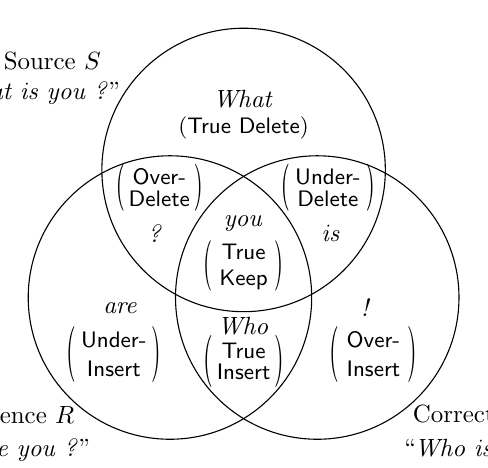
\begin{tikzpicture}[transform shape, scale=0.90]
        \draw ( 90:1.2) circle (2.0);
        \draw (210:1.2) circle (2.0);
        \draw (330:1.2) circle (2.0);
        \node[anchor=south,overlay] at ($(90: 2.5)+(-2.7, -0.00)$) {Source $S$};
        \node[anchor=south,overlay] at ($(90: 2.5)+(-3.0, -0.50)$) {``\textit{What is you ?}''};
        \node[anchor=east,overlay] at ($(210: 2.5)+(-0.10, -1.00)$) {Reference $R$};
        \node[anchor=east,overlay] at ($(210: 2.5)+( 0.15, -1.50)$) {``\textit{Who are you ?}''};
        \node[anchor=west,overlay] at ($(330: 2.5)+( 0.10, -1.00)$) {Correction $C$};
        \node[anchor=west,overlay] at ($(330: 2.5)+(-0.05, -1.50)$) {``\textit{Who is you !}''};
        \node at ($(  0: 0.0)+( 0.00, 0.45)$) {\textit{you}};
        \node at ($(  0: 0.0)+( 0.00, 0.05)$) {\small\textsf{True}};
        \node at ($(  0: 0.0)+( 0.00,-0.35)$) {\small\textsf{Keep}};
        \node at ($(  0: 0.0)+(-0.50,-0.15)$) {\scalebox{1}[2.25]{\small(}};
        \node at ($(  0: 0.0)+( 0.50,-0.15)$) {\scalebox{1}[2.25]{\small)}};
        \node at ($( 90: 2.0)+( 0.00, 0.20)$) {\textit{What}};
        \node at ($( 90: 2.0)+( 0.00,-0.20)$) {\small(\textsf{True Delete})};
        \node at ($(150: 1.2)+(-0.20,-0.30)$) {\textit{?}};
        \node at ($(150: 1.2)+(-0.15, 0.50)$) {\small\textsf{Over-}};
        \node at ($(150: 1.2)+(-0.15, 0.20)$) {\small\textsf{Delete}};
        \node at ($(150: 1.2)+(-0.70, 0.35)$) {\scalebox{1}[2.1]{\small(}};
        \node at ($(150: 1.2)+( 0.40, 0.35)$) {\scalebox{1}[2.1]{\small)}};
        \node at ($(210: 2.0)+( 0.00, 0.25)$) {\textit{are}};
        \node at ($(210: 2.0)+(-0.10,-0.20)$) {\small\textsf{Under-}};
        \node at ($(210: 2.0)+(-0.10,-0.60)$) {\small\textsf{Insert}};
        \node at ($(210: 2.0)+(-0.70,-0.40)$) {\scalebox{1}[2.25]{(}};
        \node at ($(210: 2.0)+( 0.50,-0.40)$) {\scalebox{1}[2.25]{)}};
        \node at ($(270: 1.2)+( 0.00, 0.20)$) {\textit{Who}};
        \node at ($(270: 1.2)+( 0.00,-0.15)$) {\small\textsf{True}};
        \node at ($(270: 1.2)+( 0.00,-0.45)$) {\small\textsf{Insert}};
        \node at ($(270: 1.2)+(-0.50,-0.30)$) {\scalebox{1}[2.1]{(}};
        \node at ($(270: 1.2)+( 0.50,-0.30)$) {\scalebox{1}[2.1]{)}};
        \node at ($(330: 2.0)+( 0.00, 0.25)$) {\textit{!}};
        \node at ($(330: 2.0)+( 0.10,-0.20)$) {\small\textsf{Over-}};
        \node at ($(330: 2.0)+( 0.10,-0.60)$) {\small\textsf{Insert}};
        \node at ($(330: 2.0)+(-0.45,-0.40)$) {\scalebox{1}[2.25]{(}};
        \node at ($(330: 2.0)+( 0.65,-0.40)$) {\scalebox{1}[2.25]{)}};
        \node at ($( 30: 1.2)+( 0.20,-0.30)$) {\textit{is}};
        \node at ($( 30: 1.2)+( 0.15, 0.50)$) {\small\textsf{Under-}};
        \node at ($( 30: 1.2)+( 0.15, 0.20)$) {\small\textsf{Delete}};
        \node at ($( 30: 1.2)+(-0.45, 0.35)$) {\scalebox{1}[2.1]{\small(}};
        \node at ($( 30: 1.2)+( 0.75, 0.35)$) {\scalebox{1}[2.1]{\small)}};
    \end{tikzpicture}
    \begin{tabular}{rllll}
        \vspace*{0.0em} \\
        Source $S$: & \textit{What} & \textit{is} & \textit{you} & \textit{?} \\
        Reference $R$: & \textit{Who} & \textit{are} & \textit{you} & \textit{?} \\
        Correction $C$: & \textit{Who} & \textit{is} & \textit{you} & \textit{!}
    \end{tabular}
    \caption{A three-set Venn diagram shows the occurrence of word 1-grams of $S, R, C$.}
    \label{fig:Who_are_you_?}
\end{figure}

GREEN treats a sentence as a multiset of $n$-grams with the maximum $n$-gram size $N$.
For example, a sentence ``\textit{a a b}'' is treated as a multiset $\{\textit{a}, \textit{a}, \textit{b}, \textit{a-a}, \textit{a-b}\}$\footnote{In this paper, $n$-grams are represented by connecting each word with a hyphen instead of a whitespace to avoid confusing $n$-gram with sentence.} when we set $N = 2$\footnote{Thus \textit{a-a-b} is not included in this multiset.}.
GREEN considers the difference between multisets of $n$-grams as a correction.
Corrections can be classified into deletion, insertion, and keep.
For example, corrections from $\{\textit{a}, \textit{c}\}$ to $\{\textit{b}, \textit{c}\}$ involves deletion of \textit{a}, which decreases the number of words, insertion of \textit{b}, which increases the number of words, and keep of \textit{c}, which does not change the word count\footnote{In GREEN, correction does not involve substitution. Substitution in alignment-based metrics corresponds to a combination of deletion and insertion in GREEN.}.

GREEN compares the match between the corrections from the source sentence $S$ to the reference sentence $R$ and the corrections from $S$ to the corrected sentence $C$.
To count the match between $S \to R$ and $S \to C$, we introduce a Venn diagram illustrating the occurrences of word $n$-grams in $S, R, C$ in Figure~\ref{fig:Who_are_you_?}\footnote{We do not show $n$-grams of lengths two or more for simplicity in the Venn diagram.}.
Table~\ref{tab:classification} shows what types of corrections are performed in $S \to R$ and $S \to C$, respectively, for all $n$-grams in each region of this Venn diagram.
For example, the region $S \cap \overline{R} \cap \overline{C}$ contains $n$-grams that appear in $S$ but not in $R$ and $C$, such as ``\textit{What}''.
We call this region \textsf{True Delete}~(\textsf{TD}) because these $n$-grams are correctly deleted through $S \to R$ and $S \to C$.
Similarly, the region $\overline{S} \cap R \cap C$ containing $n$-grams inserted in both $S \to R$ and $S \to C$ is called \textsf{True Insert}~(\textsf{TI}) and the region $S \cap R \cap C$ containing $n$-grams kept in both $S \to R$ and $S \to C$ is called \textsf{True Keep}~(\textsf{TK}).
\textsf{TD}, \textsf{TI}, and \textsf{TK} are \textsf{True Positive}~(\textsf{TP}) because both $S \to R$ and $S \to C$ take the same type of corrections.
The regions $S \cap R \cap \overline{C}$ and $\overline{S} \cap \overline{R} \cap C$ contain $n$-grams that are not deleted or inserted in $S \to R$, but are excessively deleted or inserted in $S \to C$.
We call them \textsf{Over-Delete}~(\textsf{OD}) and \textsf{Over-Insert}~(\textsf{OI}), respectively.
The elements in \textsf{OD} and \textsf{OI} are \textsf{False Positive}~(\textsf{FP}) because they are mistakenly deleted or inserted in $S \to C$.
The regions $S \cap \overline{R} \cap C$ and $\overline{S} \cap R \cap \overline{C}$ contain $n$-grams that should have been deleted or inserted in $S \to C$ as they are deleted or inserted in $S \to R$.
We call them \textsf{Under-Delete}~(\textsf{UD}) and \textsf{Under-Insert}~(\textsf{UI}), respectively.
The elements in \textsf{UD} and \textsf{UI} are \textsf{False Negative}~(\textsf{FN}) because they should have been deleted or inserted in $S \to C$.

\begin{table}[!t]
    \centering
    \setlength{\tabcolsep}{4pt}
    \begin{tabular}{l|l|ll}
        \hline
        Region & Name & $S \to R$ & $S \to C$ \\
        \hline
        $S \cap \overline{R} \cap \overline{C} $ & \textsf{True Delete} & Delete & Delete \\
        $\overline{S} \cap R \cap C$ & \textsf{True Insert} & Insert & Insert \\
        $S \cap R \cap C$ & \textsf{True Keep} & Keep & Keep \\
        \hline
        $S \cap R \cap \overline{C}$ & \textsf{Over-Delete} & Keep & Delete \\
        $\overline{S} \cap \overline{R} \cap C$ & \textsf{Over-Insert} & None & Insert \\
        \hline
        $S \cap \overline{R} \cap C$ & \textsf{Under-Delete} & Delete & Keep \\
        $\overline{S} \cap R \cap \overline{C}$ & \textsf{Under-Insert} & Insert & None \\
        \hline
    \end{tabular}
    \caption{A table describes each region in Figure~\ref{fig:Who_are_you_?}. Correction in which no $n$-gram appears in the common region involves ``None''.}
    \label{tab:classification}
\end{table}

Next, we explain how to calculate the number of $n$-grams in each region of the Venn diagram by the operations on multisets.
In this paper, we use three operations on multisets: intersection~($\cap$), union~($\cup$), and difference~($\setminus$).
Each operation on multisets $A$ and $B$ is defined concerning the multiplicity of any element $x$ in $A$ and $B$.
The multiplicity of an element $x$ in a multiset $A$, which is denoted as $m_A (x)$, represents the number of times $x$ occurs in $A$.
For example, 
$m_A(\textit{a}) = 2$ and
$m_A(\textit{a-a}) = 1$
when $A = \{\textcolor{red}{\textbf{\textit{a}}}, \textcolor{red}{\textbf{\textit{a}}}, \textit{b}, \textcolor{red}{\textbf{\textit{a-a}}}, \textit{a-b}\}$.
In this paper, we define the three operations above as follows:
\begingroup
\allowdisplaybreaks
\begin{align*}
    m_{A \cap B} (x) & = \min (m_A (x), m_B (x)), \\
    m_{A \cup B} (x) & = \max (m_A (x), m_B (x)), \\
    m_{A \setminus B} (x) & = \max (m_A (x) - m_B (x), 0).
\end{align*}
\endgroup
Hence, the number of $n$-gram $x$ included in each region of the Venn diagram in Figure~\ref{fig:Who_are_you_?} is represented as follows:
\begingroup
\allowdisplaybreaks
\begin{align}
    & \textsf{TD}_{S, R, C} (x) 
    = m_{S \cap \overline{R} \cap \overline{C}} (x)
    = m_{S \setminus (R \cup C)} (x) \nonumber \\ 
    = & \max\{m_S (x) \scalebox{1}[1]{\ensuremath{-}} \max(m_R (x), m_C (x)), 0\}, \label{eq:true_delete}
    \\[2\jot]
    & \textsf{TI}_{S, R, C} (x)
    = m_{\overline{S} \cap R \cap C} (x)
    = m_{(R \cap C) \setminus S} (x) \nonumber \\
    = & \max\{\min(m_R (x), m_C (x)) - m_S (x), 0\}, \label{eq:true_insert} \\[2\jot]
    & \textsf{TK}_{S, R, C} (x)
    = m_{S \cap R \cap C}(x) \nonumber \\
    = & \min(m_S(x), m_R(x), m_C (x)), \label{eq:true_keep}
    \\[2\jot]
    & \textsf{OD}_{S, R, C} (x)
    = m_{S \cap R \cap \overline{C}} (x)
    = m_{(S \cap R) \setminus C} (x) \nonumber \\
    = & \max\{\min(m_S (x), m_R (x)) - m_C (x), 0\}, \label{eq:over_delete} \\[2\jot]
    & \textsf{OI}_{S, R, C} (x)
    = m_{\overline{S} \cap \overline{R} \cap C} (x)
    = m_{C \setminus (S \cup R)} (x) \nonumber \\
    = & \max\{m_C (x) \scalebox{1}[1]{\ensuremath{-}} \max(m_S (x), m_R (x)), 0\}, \label{eq:over_insert}
    \\[2\jot]
    & \textsf{UD}_{S, R, C} (x)
    = m_{S \cap \overline{R} \cap C} (x)
    = m_{(S \cap C) \setminus R} (x) \nonumber \\
    = & \max\{\min(m_S (x), m_C (x)) - m_R (x), 0\}, \label{eq:under_delete}
    \\[2\jot]
    & \textsf{UI}_{S, R, C} (x)
    = m_{\overline{S} \cap R \cap \overline{C}} (x)
    = m_{R \setminus (S \cup C)} (x) \nonumber \\
    = & \max\{m_R (x) \scalebox{1}[1]{\ensuremath{-}} \max(m_S (x), m_C (x)), 0\}. \label{eq:under_insert}
\end{align}
\endgroup

GREEN calculates \textsf{TP}, \textsf{FP}, and \textsf{FN} for each $n$-gram size.
The \textsf{TP}, \textsf{FP}, and \textsf{FN} of $n$-grams for $S, R, C$ are calculated as follows:
\begingroup
\allowdisplaybreaks
\begin{align*}
    & \textsf{TP}_{n, S, R, C} \\
    = & \sum_{\mathclap{\forallngramx}}
    \left( \textsf{TD}_{S,R,C} (x) + \textsf{TI}_{S,R,C} (x) + \textsf{TK}_{S,R,C} (x) \right), \\
    & \textsf{FP}_{n, S, R, C}
    = \sum_{\mathclap{\forallngramx}}
    \left( \textsf{OD}_{S,R,C} (x) + \textsf{OI}_{S,R,C} (x) \right), \\
    & \textsf{FN}_{n, S, R, C}
    = \sum_{\mathclap{\forallngramx}}
    \left( \textsf{UD}_{S,R,C} (x) + \textsf{UI}_{S,R,C} (x) \right).
\end{align*}
\endgroup

Finally, GREEN accumulates \textsf{TP}, \textsf{FP}, and \textsf{FN} for corpus-level to obtain an $F$ score.
$\mathbb{S} = (S_1, \ldots, S_D), \mathbb{R} = (R_1, \ldots, R_D), \mathbb{C} = (C_1, \ldots, C_D)$ denote a set of $D$ source, reference, and corrected sentences respectively.
GREEN calculates precision and recall for $n$-gram lengths from $1$ to $N$ and the geometric mean of these precisions and recalls as BLEU~\citep{papineni-etal-2002-bleu} does.
\begingroup
\allowdisplaybreaks
\begin{align*}
    & \mathrm{prec} (N, \mathbb{S}, \mathbb{R}, \mathbb{C}) \\[-2\jot]
    = & \left( \prod_{n=1}^{N}
    \frac{
        \sum_{i=1}^{D} \textsf{TP}_{n, S_i, R_i, C_i}
    }{
        \sum_{i=1}^{D} \left( \textsf{TP}_{n, S_i, R_i, C_i} + \textsf{FP}_{n, S_i, R_i, C_i} \right)
    }
    \right)^{\tfrac{1}{N}}, \\[3\jot]
    & \mathrm{recall} (N, \mathbb{S}, \mathbb{R}, \mathbb{C}) \\[-2\jot]
    = & \left( \prod_{n=1}^{N}
    \frac{
        \sum_{i=1}^{D} \textsf{TP}_{n, S_i, R_i, C_i}
    }{
        \sum_{i=1}^{D} \left( \textsf{TP}_{n, S_i, R_i, C_i} + \textsf{FN}_{n, S_i, R_i, C_i} \right)
    }
    \right)^{\tfrac{1}{N}}.
\end{align*}
\endgroup
At last, we calculate an $F_{\beta}$ score as follows:
\begingroup
\allowdisplaybreaks
\begin{align*}
    & F_{\beta} (N, \mathbb{S}, \mathbb{R}, \mathbb{C}) \\
    = &
    \frac{
        (1+\beta^2) \mathrm{prec} (N, \mathbb{S}, \mathbb{R}, \mathbb{C})  \mathrm{recall} (N, \mathbb{S}, \mathbb{R}, \mathbb{C})
    }{
        \beta^2 \mathrm{prec} (N, \mathbb{S}, \mathbb{R}, \mathbb{C}) + \mathrm{recall} (N, \mathbb{S}, \mathbb{R}, \mathbb{C})
    }
\end{align*}
where $\beta$ is a factor denoting how important recall is in comparison to precision.
\endgroup
In this paper, we call this $F_{\beta}$ score GREEN${}_{\beta}$.

\subsection{GREEN for Multiple References}
\label{sec:multiple_references}

When we use multiple references, i.e., when $m$ reference sentences $R_{i_1},\ldots,R_{i_m}$ are given for the $i$-th source sentence $S_i$, GREEN selects the reference sentence $\hat{R}_i$ that maximizes the sentence-level GREEN for the corrected sentence $C_i$ as follows:
\begin{equation}
    \hat{R}_i = \operatorname*{argmax}_{\mathclap{R \in \{R_{i_1}, \ldots, R_{i_m}\}}} \mathrm{GREEN}_{\beta}(N, (S_i), (R), (C_i)).
    \label{eq:rhat}
\end{equation}
We compute $\mathrm{GREEN}_{\beta}(\mathbb{S}, \hat{\mathbb{R}}, \mathbb{C})$ using $D$ reference sentences $\hat{\mathbb{R}} = \{\hat{R}_1, \ldots\, \hat{R}_D\}$ selected by Equation~(\ref{eq:rhat}).
This practice of selecting the reference that maximizes the sentence-level $F$-score is also adopted in M${}^2$ and ERRANT.

\subsection{Reformulation of GLEU}
\label{sec:reformulation}

\begin{figure*}[!t]
    \begin{align}
        p_n & = \frac{\displaystyle \smashoperator[r]{\sum_{\forallngramx \in R \cap C}} m_{R \cap C} (x) - \smashoperator{\sum_{\forallngramx \in S \cap C}} \max\{0, m_{S \cap C} (x) - m_{R \cap C} (x)\}}{\displaystyle \smashoperator{\sum_{\forallngramx \in C}} m_C (x)} \label{eq:original_gleu} \\
        & = \frac{\displaystyle \smashoperator[r]{\sum_{\forallngramx \in R \cap C}} m_{R \cap C} (x) - \smashoperator{\sum_{\forallngramx \in S \cap C}} \max\{0, \min(m_S (x), m_C (x)) - \min(m_R (x), m_C (x))\}}{\displaystyle \smashoperator{\sum_{\forallngramx \in C}} m_C (x)} \nonumber \\
        & = \frac{\displaystyle \smashoperator[r]{\sum_{\forallngramx \in R \cap C}} m_{R \cap C} (x) - \smashoperator{\sum_{\forallngramx \in S \cap C}} \max\{0, \min(m_S (x), m_C (x)) - m_R (x)\}}{\displaystyle \smashoperator{\sum_{\forallngramx \in C}} m_C (x)} \nonumber \\
        & = \frac{\displaystyle \smashoperator[r]{\sum_{\forallngramx}} m_{R \cap C} (x) - \smashoperator{\sum_{\forallngramx}} m_{(S \cap C) \setminus R} (x)}{\displaystyle \smashoperator{\sum_{\forallngramx}} m_C (x)}
        = \frac{\smashoperator[r]{\sum_{\forallngramx}} \textsf{TI} (x) + \textsf{TK} (x) - \textsf{UD} (x)}{\smashoperator[r]{\sum_{\forallngramx}} \textsf{TI} (x) + \textsf{TK} (x) + \textsf{OI} (x) + \textsf{UD} (x)} \label{eq:reformulated_gleu}
    \end{align}
    \caption{Reformulation of GLEU.}
    \label{fig:gleu}
\end{figure*}

To compare GREEN with GLEU, we transform GLEU into a form using the representations in Equations (\ref{eq:true_delete}) through (\ref{eq:under_insert}).
Equation~(\ref{eq:original_gleu}) is a multiset-based representation of the original GLEU formula.
The transformation in Figure~\ref{fig:gleu} results in Equation~(\ref{eq:reformulated_gleu}).
We can see that GLEU is calculated by subtracting \textsf{UD} as penalty term from the numerator of $n$-gram precision $\sum m_{R \cap C} (x) / \sum m_{C} (x)$.
GLEU uses only \textsf{TI}, \textsf{TK}, \textsf{OI}, and \textsf{UD} from Equations~(\ref{eq:true_delete}) through (\ref{eq:under_insert}), while GREEN uses all of them.
GLEU has \textsf{FN}s in the penalty term but no \textsf{FP}s, which could lead to underestimating \textsf{FP}s and unreasonably giving high scores to systems that make aggressively incorrect edits.

\section{Experiments}
\label{sec:experiment}

\subsection{Settings}
\label{sec:settings}

To demonstrate the effectiveness of GREEN, we computed its correlation with human judgments on the CoNLL-2014 evaluation dataset~\citep{grundkiewicz-etal-2015-human} and the SEEDA dataset~\citep{10.1162/tacl_a_00676}.
The CoNLL-2014 dataset is based on the test dataset of the CoNLL-2014 shared task~\citep{ng-etal-2014-conll}, which utilizes student essays and consists of 1,312 source sentences.
In this dataset, each instance has two reference sentences.
This evaluation dataset consists of the rankings for each instance from 13 GEC system outputs~(12 submissions of the shared task participants and the source text).
The SEEDA dataset shares the source and reference sentences with the CoNLL-2014 dataset.
This dataset consists of the rankings for 15 corrected texts, including source text and two human-written texts.
To follow modern trends in GEC, SEEDA employs the modern neural systems, while the CoNLL-2014 dataset consists of classical systems.
The default setting of the SEEDA evaluation excludes two fluency texts~(GPT-3.5 corrected text and human-written text) from 15 texts, and we followed this.
SEEDA has two system rankings with different annotation methods: SEEDA-S for the sentence-based human evaluation and SEEDA-E for the edit-based human evaluation.

Following \citet{grundkiewicz-etal-2015-human}, we measure Pearson $r$ and Spearman $\rho$ correlation coefficients between the evaluation metric scores and human rankings.
We must convert them into corpus-level system scores because the human judgment dataset consists of sentence-level rankings.
We use the Expected Wins~(EW) score~\citep{bojar-etal-2013-findings} employed in the WMT13 task of the evaluation metric as the corpus-level system score because \citet{grundkiewicz-etal-2015-human} validated that we can obtain high accuracy by EW with the human judgment dataset for GEC.

In our experiments, for $n$-gram-based metrics, we use a maximum $n$-gram length of $N=4$ for word-level tokenization following the setting of GLEU, and $N=6$ for character-level following the setting of CHRF~\citep{popovic-2015-chrf}, which is a character-level metric for machine translation.
The difference in tokenization is denoted as ``wordGREEN'' (word-level) or ``charGREEN'' (character-level).

\begin{table*}[!t]
    \centering
    \tabcolsep 4pt
    \begin{tabular}{lrrrrrrrrrrrr}
        \hline
        & \multicolumn{6}{c}{Corpus-Level Metrics}
        & \multicolumn{6}{c}{Sentence-Level Metrics} \\
        & \multicolumn{2}{c}{CoNLL}
        & \multicolumn{2}{c}{SEEDA-S}
        & \multicolumn{2}{c}{SEEDA-E}
        & \multicolumn{2}{c}{CoNLL}
        & \multicolumn{2}{c}{SEEDA-S}
        & \multicolumn{2}{c}{SEEDA-E} \\
        & \multicolumn{1}{c}{$r$} & \multicolumn{1}{c}{$\rho$}
        & \multicolumn{1}{c}{$r$} & \multicolumn{1}{c}{$\rho$}
        & \multicolumn{1}{c}{$r$} & \multicolumn{1}{c}{$\rho$}
        & \multicolumn{1}{c}{$r$} & \multicolumn{1}{c}{$\rho$}
        & \multicolumn{1}{c}{$r$} & \multicolumn{1}{c}{$\rho$}
        & \multicolumn{1}{c}{$r$} & \multicolumn{1}{c}{$\rho$} \\
        \hline
        \multicolumn{13}{l}{Alignment-based $F$-score} \\
        M${}^2$ &
        0.623 & 0.687 & 0.616 & 0.517 & 0.736 & 0.776 &
        0.872 & 0.731 & 0.797 & 0.762 & 0.869 & \textbf{0.951} \\
        ERRANT & 
        0.644 & 0.687 & 0.529 & 0.364 & 0.690 & 0.699 & 
        0.871 & 0.775 & 0.764 & 0.727 & 0.855 & 0.930 \\
        PT-M${}^2$ &
        0.686 & 0.786 & 0.737 & 0.720 & 0.798 & 0.916 &
        \textbf{0.934} & \textbf{0.890} & 0.831 & 0.804 & 0.878 & 0.930 \\
        CLEME &
        0.648 & 0.709 & 0.573 & 0.427 & 0.702 & 0.727 &
        0.877 & 0.824 & 0.818 & 0.804 & 0.872 & 0.930 \\
        \hline
        \multicolumn{13}{l}{$n$-gram-based precision} \\
        wordGLEU &
        0.696 & 0.445 & 0.870 & 0.811 & 0.891 & 0.895 &
        0.779 & 0.720 & 0.926 & \textbf{0.923} & 0.915 & 0.916 \\
        charGLEU &
        0.606 & 0.593 & 0.807 & 0.706 & 0.843 & 0.867 &
        0.655 & 0.665 & 0.880 & 0.853 & 0.905 & 0.937 \\
        \hline
        \multicolumn{4}{l}{$n$-gram-based $F$-score} \\
        wordGREEN &
        0.741 & 0.698 & \textbf{0.920} & \textbf{0.909} & \textbf{0.911} & \textbf{0.930} &
        0.835 & 0.731 & 0.922 & 0.902 & 0.920 & 0.937 \\
        charGREEN &
        \textbf{0.786} & \textbf{0.813} & 0.913 & 0.881 & \textbf{0.911} & 0.909 &
        0.834 & 0.852 & \textbf{0.928} & 0.881 & \textbf{0.930} & 0.916 \\
        \hline
    \end{tabular}
    \caption{Pearson~($r$) and Spearman~($\rho$) correlation coefficients between each metric and the human score of the CoNLL-2014 evaluation dataset and the SEEDA dataset.}
    \label{tab:correlations}
\end{table*}

\citet{napoles-etal-2016-theres} reported that the average of sentence-level scores is better for evaluating the GEC systems than the corpus-level score when using M${}^2$ and GLEU.
However, corpus-level metric is adopted to measure the system performance in the CoNLL-2014 shared task~\citep{ng-etal-2014-conll} and the BEA-2019 shared task~\citep{bryant-etal-2019-bea}.
Because it is important for an evaluation measure to perform well at both the corpus-level and sentence-level metrics, we conduct experiments at both levels in this paper.

After the CoNLL-2014 shared task first adopted $\beta = 0.5$ for M${}^2$, it has been the standard practice to use $F_{0.5}$ for alignment-based $F$-scores.
Since it is more important for a GEC system to be precise than to correct as many errors as possible, it is considered better to weigh precision twice more than recall for M${}^2$ and its variants.
However, weighing precision more in $n$-gram-based $F$-score results that the metric most highly evaluates the unedited source sentence because precision is 100 for the source sentence, which contains no \textsf{FP}s.
Therefore, we should not weigh precision more than recall in $n$-gram-based $F$-score.
Furthermore, we should rather weigh recall more than precision because the effect of individual annotator bias~\citep{bryant-ng-2015-far} may unreasonably reduce precision due to the system corrections such that they are correct but not edited by the annotator.
To alleviate this annotator bias, we employ $\beta = 2.0$, which weighs recall twice more than precision, for GREEN in our experiments.

\begin{table}[!t]
    \centering
    \begin{tabular}{lrr}
        \hline 
        \multicolumn{1}{l}{Metric} &
        \multicolumn{1}{c}{\textsf{AMU}} &
        \multicolumn{1}{c}{\textsf{AMU-S}} \\ \hline
        M${}^2$ & 4.34 & 196.60 \\
        ERRANT & 12.35 & 14.34 \\
        PT-M${}^2$ & 109.82 & $>$ 1 hour \\
        CLEME & 10.15 & 12.10 \\
        wordGLEU & 2.69 & 2.80 \\
        wordGREEN & 0.55 & 0.56 \\ \hline
    \end{tabular}
    \caption{The average execution time in seconds to evaluate the \textsf{AMU} system output in the CoNLL-2014 dataset and the slow \textsf{AMU}~(\textsf{AMU-S}) in which one sentence in \textsf{AMU} is replaced by an example making M${}^2$ slow.}
    \label{tab:time}
\end{table}

\subsection{Results of Corpus-Level Metrics}
\label{sec:corpus_level_evaluation}

The correlation coefficients between the reference-based corpus-level GEC metrics and the EW scores on the CoNLL and SEEDA datasets are shown in the left half of Table~\ref{tab:correlations}.
We confirmed that wordGREEN or charGREEN performs the best in these corpus-level metrics.
We confirmed that wordGREEN and charGREEN perform the best on the CoNLL-2014 and SEEDA datasets, respectively, in corpus-level metrics.
The three alignment-based $F$-scores of M${}^2$, ERRANT, and CLEME show similar performance, while PT-M${}^2$ is better than these metrics, which implies that the impact of incorporating the pre-trained model is significant.
GLEU shows a relatively worse performance with Spearman $\rho$ in CoNLL-2014 as shown in \citet{chollampatt-ng-2018-reassessment}, while GLEU shows a relatively better performance in SEEDA as shown in \citet{10.1162/tacl_a_00676}.
We can confirm that GREEN, in contrast to GLEU, performs consistently well in both classical and neural system evaluations.

\subsection{Results of Sentence-Level Metrics}
\label{sec:sentence_level_evaluation}

The correlation coefficients between the reference-based sentence-level GEC metrics and the EW scores on the CoNLL and SEEDA datasets are shown in the right half of Table~\ref{tab:correlations}.
We can confirm that wordGREEN and charGREEN show comparable performance to the existing sentence-level metrics.
In particular, charGREEN shows the best Pearson correlation coefficients $r$ on the SEEDA-S and SEEDA-E datasets.
On CoNLL-2014, PT-M${}^2$ shows the highest correlation using a pre-trained model BERT.
All the sentence-level metrics show higher correlations than their corpus-level counterparts, as shown in \citet{napoles-etal-2016-theres}.
The GEC field needs to investigate why sentence-level metrics are good in future work.

\subsection{Efficiency of GREEN}
\label{sec:speed}

We measured the average execution time of 10 runs to calculate the score for evaluating the output of the \textsf{AMU} system that shows the highest score with human evaluation in the CoNLL-2014 shared task.
As mentioned in Section~\ref{sec:m2}, the worst-case time complexity of M${}^2$ is quite high.
We also measure the average execution time of \textsf{AMU-S}, which replaces one sentence of \textsf{AMU} with an example\footnote{We included this in Appendix~\ref{sec:appendix}.} making M${}^2$ slow because it corresponds to the worst-case scenario.
We show the execution times in seconds in Table \ref{tab:time}.
GREEN has the advantage of being faster than other methods in execution time, although its performance is better than or comparable to others.
M${}^2$ and PT-M${}^2$ are not practical in the worst-case scenario.
The advantage of GREEN is that it does not require linguistic resources to compute alignments or pre-trained models, which enables even non-English GEC to perform the evaluation immediately and efficiently in linear time, without the preparation of annotated data required in M${}^2$ and PT-M${}^2$ or linguistic resources required in ERRANT and CLEME.
Despite an $n$-gram frequency-based method, GLEU takes a longer execution time than GREEN because GLEU samples random references 500 times when using multiple references.

\section{Analysis}
\label{sec:analysis}

\begin{figure}[!t]
    \centering
    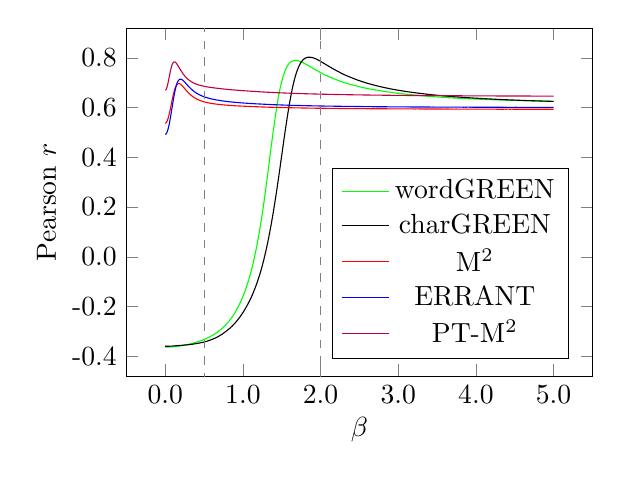
\begin{tikzpicture}
        \begin{axis}[
                width = 7.5cm,
                height = 6.0cm,
                xtick={0.0, 1.0, 2.0, 3.0, 4.0, 5.0},
                ytick={-0.4, -0.2, 0.0, 0.2, 0.4, 0.6, 0.8},
                xticklabels={0.0, 1.0, 2.0, 3.0, 4.0, 5.0},
                yticklabels={-0.4, -0.2, 0.0, 0.2, 0.4, 0.6, 0.8},
                xlabel near ticks, xlabel shift={-2pt},
                ylabel near ticks, ylabel shift={-1pt},
                xlabel = $\beta$,
                ylabel = Pearson $r$,
                legend entries={wordGREEN, charGREEN, M${}^2$, ERRANT, PT-M${}^2$},
                legend style={at={(0.95, 0.05)}, anchor=south east}]
            \newcommand{\wordgreenbetapearson}{(0.00, -0.36043) (0.01, -0.36327) (0.02, -0.36317) (0.03, -0.36311) (0.04, -0.36293) (0.05, -0.36287) (0.06, -0.36261) (0.07, -0.36254) (0.08, -0.36237) (0.09, -0.36213) (0.10, -0.36193) (0.11, -0.36172) (0.12, -0.36126) (0.13, -0.36077) (0.14, -0.36053) (0.15, -0.35991) (0.16, -0.35966) (0.17, -0.35914) (0.18, -0.35875) (0.19, -0.35834) (0.20, -0.35790) (0.21, -0.35730) (0.22, -0.35665) (0.23, -0.35600) (0.24, -0.35543) (0.25, -0.35469) (0.26, -0.35416) (0.27, -0.35371) (0.28, -0.35302) (0.29, -0.35257) (0.30, -0.35199) (0.31, -0.35112) (0.32, -0.35034) (0.33, -0.34941) (0.34, -0.34854) (0.35, -0.34760) (0.36, -0.34678) (0.37, -0.34589) (0.38, -0.34507) (0.39, -0.34417) (0.40, -0.34324) (0.41, -0.34228) (0.42, -0.34134) (0.43, -0.34030) (0.44, -0.33928) (0.45, -0.33824) (0.46, -0.33713) (0.47, -0.33599) (0.48, -0.33468) (0.49, -0.33344) (0.50, -0.33203) (0.51, -0.33067) (0.52, -0.32938) (0.53, -0.32802) (0.54, -0.32665) (0.55, -0.32518) (0.56, -0.32380) (0.57, -0.32219) (0.58, -0.32053) (0.59, -0.31884) (0.60, -0.31708) (0.61, -0.31533) (0.62, -0.31347) (0.63, -0.31142) (0.64, -0.30942) (0.65, -0.30770) (0.66, -0.30554) (0.67, -0.30332) (0.68, -0.30101) (0.69, -0.29865) (0.70, -0.29620) (0.71, -0.29362) (0.72, -0.29108) (0.73, -0.28831) (0.74, -0.28547) (0.75, -0.28262) (0.76, -0.27956) (0.77, -0.27636) (0.78, -0.27323) (0.79, -0.26982) (0.80, -0.26627) (0.81, -0.26288) (0.82, -0.25911) (0.83, -0.25512) (0.84, -0.25106) (0.85, -0.24683) (0.86, -0.24265) (0.87, -0.23816) (0.88, -0.23339) (0.89, -0.22825) (0.90, -0.22317) (0.91, -0.21789) (0.92, -0.21198) (0.93, -0.20621) (0.94, -0.20041) (0.95, -0.19437) (0.96, -0.18779) (0.97, -0.18093) (0.98, -0.17429) (0.99, -0.16712) (1.00, -0.15959) (1.01, -0.15203) (1.02, -0.14386) (1.03, -0.13506) (1.04, -0.12608) (1.05, -0.11682) (1.06, -0.10700) (1.07, -0.09670) (1.08, -0.08665) (1.09, -0.07600) (1.10, -0.06479) (1.11, -0.05252) (1.12, -0.04057) (1.13, -0.02727) (1.14, -0.01374) (1.15, 0.00014) (1.16, 0.01506) (1.17, 0.03024) (1.18, 0.04598) (1.19, 0.06251) (1.20, 0.07954) (1.21, 0.09676) (1.22, 0.11589) (1.23, 0.13508) (1.24, 0.15463) (1.25, 0.17486) (1.26, 0.19559) (1.27, 0.21763) (1.28, 0.24003) (1.29, 0.26264) (1.30, 0.28656) (1.31, 0.31025) (1.32, 0.33333) (1.33, 0.35914) (1.34, 0.38312) (1.35, 0.40797) (1.36, 0.43296) (1.37, 0.45700) (1.38, 0.48076) (1.39, 0.50426) (1.40, 0.52651) (1.41, 0.54855) (1.42, 0.57021) (1.43, 0.59067) (1.44, 0.61003) (1.45, 0.62969) (1.46, 0.64710) (1.47, 0.66343) (1.48, 0.67835) (1.49, 0.69222) (1.50, 0.70494) (1.51, 0.71694) (1.52, 0.72742) (1.53, 0.73691) (1.54, 0.74539) (1.55, 0.75368) (1.56, 0.76034) (1.57, 0.76678) (1.58, 0.77154) (1.59, 0.77553) (1.60, 0.77910) (1.61, 0.78210) (1.62, 0.78430) (1.63, 0.78619) (1.64, 0.78729) (1.65, 0.78850) (1.66, 0.78909) (1.67, 0.78988) (1.68, 0.78971) (1.69, 0.78948) (1.70, 0.78902) (1.71, 0.78828) (1.72, 0.78708) (1.73, 0.78607) (1.74, 0.78504) (1.75, 0.78443) (1.76, 0.78301) (1.77, 0.78141) (1.78, 0.77967) (1.79, 0.77817) (1.80, 0.77644) (1.81, 0.77474) (1.82, 0.77303) (1.83, 0.77107) (1.84, 0.76927) (1.85, 0.76811) (1.86, 0.76583) (1.87, 0.76408) (1.88, 0.76198) (1.89, 0.76019) (1.90, 0.75838) (1.91, 0.75660) (1.92, 0.75482) (1.93, 0.75311) (1.94, 0.75136) (1.95, 0.74961) (1.96, 0.74788) (1.97, 0.74596) (1.98, 0.74428) (1.99, 0.74243) (2.00, 0.74062) (2.01, 0.73874) (2.02, 0.73724) (2.03, 0.73526) (2.04, 0.73380) (2.05, 0.73243) (2.06, 0.73094) (2.07, 0.72945) (2.08, 0.72853) (2.09, 0.72707) (2.10, 0.72557) (2.11, 0.72400) (2.12, 0.72261) (2.13, 0.72136) (2.14, 0.72002) (2.15, 0.71870) (2.16, 0.71741) (2.17, 0.71622) (2.18, 0.71492) (2.19, 0.71374) (2.20, 0.71248) (2.21, 0.71128) (2.22, 0.71012) (2.23, 0.70896) (2.24, 0.70785) (2.25, 0.70673) (2.26, 0.70551) (2.27, 0.70435) (2.28, 0.70324) (2.29, 0.70219) (2.30, 0.70115) (2.31, 0.70015) (2.32, 0.69915) (2.33, 0.69816) (2.34, 0.69721) (2.35, 0.69625) (2.36, 0.69532) (2.37, 0.69440) (2.38, 0.69381) (2.39, 0.69293) (2.40, 0.69206) (2.41, 0.69119) (2.42, 0.69034) (2.43, 0.68968) (2.44, 0.68888) (2.45, 0.68807) (2.46, 0.68712) (2.47, 0.68634) (2.48, 0.68557) (2.49, 0.68475) (2.50, 0.68402) (2.51, 0.68325) (2.52, 0.68243) (2.53, 0.68172) (2.54, 0.68101) (2.55, 0.68032) (2.56, 0.67964) (2.57, 0.67897) (2.58, 0.67830) (2.59, 0.67766) (2.60, 0.67702) (2.61, 0.67639) (2.62, 0.67576) (2.63, 0.67515) (2.64, 0.67480) (2.65, 0.67419) (2.66, 0.67361) (2.67, 0.67311) (2.68, 0.67254) (2.69, 0.67197) (2.70, 0.67141) (2.71, 0.67085) (2.72, 0.67031) (2.73, 0.66977) (2.74, 0.66926) (2.75, 0.66872) (2.76, 0.66821) (2.77, 0.66771) (2.78, 0.66722) (2.79, 0.66665) (2.80, 0.66616) (2.81, 0.66569) (2.82, 0.66521) (2.83, 0.66475) (2.84, 0.66429) (2.85, 0.66384) (2.86, 0.66338) (2.87, 0.66294) (2.88, 0.66251) (2.89, 0.66208) (2.90, 0.66138) (2.91, 0.66076) (2.92, 0.66039) (2.93, 0.65999) (2.94, 0.65958) (2.95, 0.65931) (2.96, 0.65892) (2.97, 0.65853) (2.98, 0.65815) (2.99, 0.65775) (3.00, 0.65738) (3.01, 0.65701) (3.02, 0.65664) (3.03, 0.65628) (3.04, 0.65592) (3.05, 0.65556) (3.06, 0.65521) (3.07, 0.65487) (3.08, 0.65452) (3.09, 0.65418) (3.10, 0.65370) (3.11, 0.65337) (3.12, 0.65305) (3.13, 0.65272) (3.14, 0.65240) (3.15, 0.65217) (3.16, 0.65185) (3.17, 0.65157) (3.18, 0.65120) (3.19, 0.65076) (3.20, 0.65047) (3.21, 0.65019) (3.22, 0.64990) (3.23, 0.64961) (3.24, 0.64925) (3.25, 0.64896) (3.26, 0.64869) (3.27, 0.64841) (3.28, 0.64814) (3.29, 0.64788) (3.30, 0.64758) (3.31, 0.64732) (3.32, 0.64706) (3.33, 0.64680) (3.34, 0.64654) (3.35, 0.64629) (3.36, 0.64603) (3.37, 0.64578) (3.38, 0.64554) (3.39, 0.64530) (3.40, 0.64506) (3.41, 0.64483) (3.42, 0.64460) (3.43, 0.64437) (3.44, 0.64414) (3.45, 0.64391) (3.46, 0.64369) (3.47, 0.64347) (3.48, 0.64335) (3.49, 0.64313) (3.50, 0.64291) (3.51, 0.64270) (3.52, 0.64250) (3.53, 0.64229) (3.54, 0.64208) (3.55, 0.64187) (3.56, 0.64167) (3.57, 0.64146) (3.58, 0.64126) (3.59, 0.64107) (3.60, 0.64088) (3.61, 0.64067) (3.62, 0.64049) (3.63, 0.64031) (3.64, 0.64013) (3.65, 0.63985) (3.66, 0.63967) (3.67, 0.63948) (3.68, 0.63931) (3.69, 0.63912) (3.70, 0.63898) (3.71, 0.63880) (3.72, 0.63863) (3.73, 0.63846) (3.74, 0.63828) (3.75, 0.63811) (3.76, 0.63794) (3.77, 0.63779) (3.78, 0.63762) (3.79, 0.63745) (3.80, 0.63730) (3.81, 0.63713) (3.82, 0.63698) (3.83, 0.63683) (3.84, 0.63668) (3.85, 0.63652) (3.86, 0.63637) (3.87, 0.63622) (3.88, 0.63606) (3.89, 0.63592) (3.90, 0.63578) (3.91, 0.63562) (3.92, 0.63551) (3.93, 0.63537) (3.94, 0.63522) (3.95, 0.63508) (3.96, 0.63494) (3.97, 0.63485) (3.98, 0.63471) (3.99, 0.63458) (4.00, 0.63444) (4.01, 0.63431) (4.02, 0.63417) (4.03, 0.63404) (4.04, 0.63392) (4.05, 0.63369) (4.06, 0.63356) (4.07, 0.63344) (4.08, 0.63332) (4.09, 0.63319) (4.10, 0.63306) (4.11, 0.63294) (4.12, 0.63282) (4.13, 0.63270) (4.14, 0.63256) (4.15, 0.63244) (4.16, 0.63232) (4.17, 0.63221) (4.18, 0.63209) (4.19, 0.63197) (4.20, 0.63186) (4.21, 0.63175) (4.22, 0.63163) (4.23, 0.63152) (4.24, 0.63141) (4.25, 0.63130) (4.26, 0.63120) (4.27, 0.63108) (4.28, 0.63098) (4.29, 0.63088) (4.30, 0.63076) (4.31, 0.63066) (4.32, 0.63055) (4.33, 0.63045) (4.34, 0.63035) (4.35, 0.63025) (4.36, 0.63015) (4.37, 0.63005) (4.38, 0.62995) (4.39, 0.62985) (4.40, 0.62975) (4.41, 0.62966) (4.42, 0.62956) (4.43, 0.62946) (4.44, 0.62938) (4.45, 0.62914) (4.46, 0.62904) (4.47, 0.62895) (4.48, 0.62886) (4.49, 0.62877) (4.50, 0.62868) (4.51, 0.62859) (4.52, 0.62850) (4.53, 0.62840) (4.54, 0.62831) (4.55, 0.62823) (4.56, 0.62813) (4.57, 0.62805) (4.58, 0.62796) (4.59, 0.62789) (4.60, 0.62779) (4.61, 0.62771) (4.62, 0.62764) (4.63, 0.62755) (4.64, 0.62747) (4.65, 0.62739) (4.66, 0.62730) (4.67, 0.62723) (4.68, 0.62715) (4.69, 0.62707) (4.70, 0.62698) (4.71, 0.62690) (4.72, 0.62681) (4.73, 0.62674) (4.74, 0.62667) (4.75, 0.62658) (4.76, 0.62651) (4.77, 0.62644) (4.78, 0.62636) (4.79, 0.62630) (4.80, 0.62622) (4.81, 0.62614) (4.82, 0.62607) (4.83, 0.62600) (4.84, 0.62593) (4.85, 0.62586) (4.86, 0.62578) (4.87, 0.62573) (4.88, 0.62566) (4.89, 0.62558) (4.90, 0.62552) (4.91, 0.62544) (4.92, 0.62538) (4.93, 0.62532) (4.94, 0.62525) (4.95, 0.62518) (4.96, 0.62512) (4.97, 0.62506) (4.98, 0.62499) (4.99, 0.62492) (5.00, 0.62486)}
\newcommand{\chargreenbetapearson}{(0.00, -0.35842) (0.01, -0.35975) (0.02, -0.35978) (0.03, -0.35973) (0.04, -0.35965) (0.05, -0.35948) (0.06, -0.35934) (0.07, -0.35906) (0.08, -0.35903) (0.09, -0.35889) (0.10, -0.35862) (0.11, -0.35824) (0.12, -0.35801) (0.13, -0.35790) (0.14, -0.35762) (0.15, -0.35718) (0.16, -0.35701) (0.17, -0.35685) (0.18, -0.35674) (0.19, -0.35637) (0.20, -0.35623) (0.21, -0.35599) (0.22, -0.35577) (0.23, -0.35546) (0.24, -0.35509) (0.25, -0.35483) (0.26, -0.35456) (0.27, -0.35433) (0.28, -0.35398) (0.29, -0.35369) (0.30, -0.35329) (0.31, -0.35293) (0.32, -0.35267) (0.33, -0.35229) (0.34, -0.35183) (0.35, -0.35150) (0.36, -0.35081) (0.37, -0.35029) (0.38, -0.34986) (0.39, -0.34934) (0.40, -0.34895) (0.41, -0.34840) (0.42, -0.34784) (0.43, -0.34720) (0.44, -0.34656) (0.45, -0.34609) (0.46, -0.34548) (0.47, -0.34478) (0.48, -0.34402) (0.49, -0.34332) (0.50, -0.34251) (0.51, -0.34168) (0.52, -0.34084) (0.53, -0.34001) (0.54, -0.33904) (0.55, -0.33807) (0.56, -0.33703) (0.57, -0.33598) (0.58, -0.33489) (0.59, -0.33369) (0.60, -0.33238) (0.61, -0.33116) (0.62, -0.32991) (0.63, -0.32859) (0.64, -0.32717) (0.65, -0.32570) (0.66, -0.32418) (0.67, -0.32258) (0.68, -0.32093) (0.69, -0.31921) (0.70, -0.31741) (0.71, -0.31556) (0.72, -0.31359) (0.73, -0.31160) (0.74, -0.30947) (0.75, -0.30725) (0.76, -0.30498) (0.77, -0.30268) (0.78, -0.30032) (0.79, -0.29794) (0.80, -0.29547) (0.81, -0.29296) (0.82, -0.29035) (0.83, -0.28756) (0.84, -0.28476) (0.85, -0.28199) (0.86, -0.27898) (0.87, -0.27583) (0.88, -0.27264) (0.89, -0.26927) (0.90, -0.26579) (0.91, -0.26223) (0.92, -0.25864) (0.93, -0.25481) (0.94, -0.25080) (0.95, -0.24673) (0.96, -0.24250) (0.97, -0.23820) (0.98, -0.23379) (0.99, -0.22905) (1.00, -0.22430) (1.01, -0.21942) (1.02, -0.21433) (1.03, -0.20909) (1.04, -0.20360) (1.05, -0.19804) (1.06, -0.19226) (1.07, -0.18676) (1.08, -0.18062) (1.09, -0.17431) (1.10, -0.16763) (1.11, -0.16089) (1.12, -0.15388) (1.13, -0.14654) (1.14, -0.13892) (1.15, -0.13119) (1.16, -0.12311) (1.17, -0.11478) (1.18, -0.10609) (1.19, -0.09703) (1.20, -0.08783) (1.21, -0.07800) (1.22, -0.06792) (1.23, -0.05738) (1.24, -0.04645) (1.25, -0.03492) (1.26, -0.02303) (1.27, -0.01092) (1.28, 0.00246) (1.29, 0.01600) (1.30, 0.02979) (1.31, 0.04399) (1.32, 0.05866) (1.33, 0.07383) (1.34, 0.09025) (1.35, 0.10641) (1.36, 0.12320) (1.37, 0.14057) (1.38, 0.15870) (1.39, 0.17713) (1.40, 0.19627) (1.41, 0.21581) (1.42, 0.23562) (1.43, 0.25586) (1.44, 0.27722) (1.45, 0.29832) (1.46, 0.32010) (1.47, 0.34173) (1.48, 0.36381) (1.49, 0.38596) (1.50, 0.40822) (1.51, 0.43050) (1.52, 0.45279) (1.53, 0.47489) (1.54, 0.49673) (1.55, 0.51800) (1.56, 0.53898) (1.57, 0.55930) (1.58, 0.57913) (1.59, 0.59869) (1.60, 0.61702) (1.61, 0.63442) (1.62, 0.65143) (1.63, 0.66705) (1.64, 0.68185) (1.65, 0.69622) (1.66, 0.70892) (1.67, 0.72066) (1.68, 0.73143) (1.69, 0.74134) (1.70, 0.75027) (1.71, 0.75836) (1.72, 0.76577) (1.73, 0.77218) (1.74, 0.77788) (1.75, 0.78274) (1.76, 0.78705) (1.77, 0.79072) (1.78, 0.79379) (1.79, 0.79638) (1.80, 0.79841) (1.81, 0.80009) (1.82, 0.80120) (1.83, 0.80188) (1.84, 0.80242) (1.85, 0.80262) (1.86, 0.80255) (1.87, 0.80234) (1.88, 0.80159) (1.89, 0.80153) (1.90, 0.80063) (1.91, 0.79963) (1.92, 0.79846) (1.93, 0.79714) (1.94, 0.79583) (1.95, 0.79434) (1.96, 0.79277) (1.97, 0.79117) (1.98, 0.78945) (1.99, 0.78778) (2.00, 0.78571) (2.01, 0.78395) (2.02, 0.78213) (2.03, 0.78035) (2.04, 0.77847) (2.05, 0.77662) (2.06, 0.77475) (2.07, 0.77285) (2.08, 0.77094) (2.09, 0.76902) (2.10, 0.76720) (2.11, 0.76535) (2.12, 0.76350) (2.13, 0.76166) (2.14, 0.75989) (2.15, 0.75810) (2.16, 0.75629) (2.17, 0.75453) (2.18, 0.75283) (2.19, 0.75109) (2.20, 0.74941) (2.21, 0.74772) (2.22, 0.74605) (2.23, 0.74440) (2.24, 0.74281) (2.25, 0.74121) (2.26, 0.73941) (2.27, 0.73789) (2.28, 0.73636) (2.29, 0.73484) (2.30, 0.73335) (2.31, 0.73180) (2.32, 0.73041) (2.33, 0.72901) (2.34, 0.72770) (2.35, 0.72634) (2.36, 0.72526) (2.37, 0.72393) (2.38, 0.72260) (2.39, 0.72136) (2.40, 0.72002) (2.41, 0.71876) (2.42, 0.71754) (2.43, 0.71632) (2.44, 0.71510) (2.45, 0.71396) (2.46, 0.71269) (2.47, 0.71157) (2.48, 0.71051) (2.49, 0.70939) (2.50, 0.70821) (2.51, 0.70715) (2.52, 0.70609) (2.53, 0.70507) (2.54, 0.70403) (2.55, 0.70295) (2.56, 0.70193) (2.57, 0.70099) (2.58, 0.70001) (2.59, 0.69905) (2.60, 0.69811) (2.61, 0.69721) (2.62, 0.69629) (2.63, 0.69541) (2.64, 0.69453) (2.65, 0.69366) (2.66, 0.69279) (2.67, 0.69198) (2.68, 0.69116) (2.69, 0.69033) (2.70, 0.68953) (2.71, 0.68873) (2.72, 0.68793) (2.73, 0.68715) (2.74, 0.68642) (2.75, 0.68567) (2.76, 0.68495) (2.77, 0.68421) (2.78, 0.68348) (2.79, 0.68280) (2.80, 0.68208) (2.81, 0.68140) (2.82, 0.68073) (2.83, 0.68006) (2.84, 0.67938) (2.85, 0.67874) (2.86, 0.67808) (2.87, 0.67747) (2.88, 0.67668) (2.89, 0.67606) (2.90, 0.67548) (2.91, 0.67487) (2.92, 0.67428) (2.93, 0.67369) (2.94, 0.67312) (2.95, 0.67256) (2.96, 0.67199) (2.97, 0.67144) (2.98, 0.67090) (2.99, 0.67036) (3.00, 0.66981) (3.01, 0.66930) (3.02, 0.66877) (3.03, 0.66826) (3.04, 0.66774) (3.05, 0.66725) (3.06, 0.66677) (3.07, 0.66627) (3.08, 0.66578) (3.09, 0.66531) (3.10, 0.66483) (3.11, 0.66435) (3.12, 0.66392) (3.13, 0.66345) (3.14, 0.66298) (3.15, 0.66254) (3.16, 0.66219) (3.17, 0.66175) (3.18, 0.66129) (3.19, 0.66090) (3.20, 0.66047) (3.21, 0.66009) (3.22, 0.65969) (3.23, 0.65927) (3.24, 0.65887) (3.25, 0.65847) (3.26, 0.65809) (3.27, 0.65771) (3.28, 0.65733) (3.29, 0.65694) (3.30, 0.65658) (3.31, 0.65619) (3.32, 0.65585) (3.33, 0.65548) (3.34, 0.65512) (3.35, 0.65479) (3.36, 0.65443) (3.37, 0.65375) (3.38, 0.65340) (3.39, 0.65307) (3.40, 0.65274) (3.41, 0.65240) (3.42, 0.65208) (3.43, 0.65173) (3.44, 0.65143) (3.45, 0.65110) (3.46, 0.65080) (3.47, 0.65052) (3.48, 0.65020) (3.49, 0.64987) (3.50, 0.64960) (3.51, 0.64928) (3.52, 0.64899) (3.53, 0.64873) (3.54, 0.64845) (3.55, 0.64814) (3.56, 0.64787) (3.57, 0.64755) (3.58, 0.64730) (3.59, 0.64703) (3.60, 0.64678) (3.61, 0.64650) (3.62, 0.64620) (3.63, 0.64596) (3.64, 0.64569) (3.65, 0.64544) (3.66, 0.64520) (3.67, 0.64493) (3.68, 0.64467) (3.69, 0.64444) (3.70, 0.64419) (3.71, 0.64395) (3.72, 0.64372) (3.73, 0.64346) (3.74, 0.64330) (3.75, 0.64306) (3.76, 0.64282) (3.77, 0.64260) (3.78, 0.64239) (3.79, 0.64215) (3.80, 0.64194) (3.81, 0.64169) (3.82, 0.64147) (3.83, 0.64126) (3.84, 0.64104) (3.85, 0.64083) (3.86, 0.64062) (3.87, 0.64040) (3.88, 0.64020) (3.89, 0.64000) (3.90, 0.63979) (3.91, 0.63959) (3.92, 0.63940) (3.93, 0.63919) (3.94, 0.63900) (3.95, 0.63882) (3.96, 0.63860) (3.97, 0.63842) (3.98, 0.63821) (3.99, 0.63805) (4.00, 0.63786) (4.01, 0.63767) (4.02, 0.63749) (4.03, 0.63729) (4.04, 0.63713) (4.05, 0.63694) (4.06, 0.63679) (4.07, 0.63660) (4.08, 0.63643) (4.09, 0.63627) (4.10, 0.63606) (4.11, 0.63592) (4.12, 0.63573) (4.13, 0.63559) (4.14, 0.63543) (4.15, 0.63526) (4.16, 0.63509) (4.17, 0.63493) (4.18, 0.63477) (4.19, 0.63468) (4.20, 0.63450) (4.21, 0.63422) (4.22, 0.63404) (4.23, 0.63390) (4.24, 0.63376) (4.25, 0.63362) (4.26, 0.63345) (4.27, 0.63333) (4.28, 0.63314) (4.29, 0.63302) (4.30, 0.63287) (4.31, 0.63274) (4.32, 0.63259) (4.33, 0.63245) (4.34, 0.63231) (4.35, 0.63218) (4.36, 0.63203) (4.37, 0.63191) (4.38, 0.63176) (4.39, 0.63162) (4.40, 0.63150) (4.41, 0.63136) (4.42, 0.63123) (4.43, 0.63108) (4.44, 0.63095) (4.45, 0.63084) (4.46, 0.63069) (4.47, 0.63058) (4.48, 0.63043) (4.49, 0.63035) (4.50, 0.63022) (4.51, 0.63008) (4.52, 0.62995) (4.53, 0.62984) (4.54, 0.62970) (4.55, 0.62960) (4.56, 0.62949) (4.57, 0.62935) (4.58, 0.62925) (4.59, 0.62912) (4.60, 0.62900) (4.61, 0.62892) (4.62, 0.62879) (4.63, 0.62868) (4.64, 0.62857) (4.65, 0.62843) (4.66, 0.62833) (4.67, 0.62823) (4.68, 0.62811) (4.69, 0.62802) (4.70, 0.62790) (4.71, 0.62783) (4.72, 0.62770) (4.73, 0.62760) (4.74, 0.62749) (4.75, 0.62740) (4.76, 0.62729) (4.77, 0.62720) (4.78, 0.62709) (4.79, 0.62698) (4.80, 0.62689) (4.81, 0.62682) (4.82, 0.62671) (4.83, 0.62662) (4.84, 0.62650) (4.85, 0.62640) (4.86, 0.62631) (4.87, 0.62620) (4.88, 0.62613) (4.89, 0.62601) (4.90, 0.62593) (4.91, 0.62584) (4.92, 0.62574) (4.93, 0.62565) (4.94, 0.62556) (4.95, 0.62548) (4.96, 0.62537) (4.97, 0.62529) (4.98, 0.62521) (4.99, 0.62512) (5.00, 0.62504)}
\newcommand{\maxmatchbetapearson}{(0.00, 0.53683) (0.01, 0.53844) (0.02, 0.54304) (0.03, 0.55048) (0.04, 0.56042) (0.05, 0.57260) (0.06, 0.58656) (0.07, 0.60162) (0.08, 0.61710) (0.09, 0.63238) (0.10, 0.64681) (0.11, 0.65984) (0.12, 0.67109) (0.13, 0.68037) (0.14, 0.68736) (0.15, 0.69236) (0.16, 0.69532) (0.17, 0.69666) (0.18, 0.69676) (0.19, 0.69544) (0.20, 0.69338) (0.21, 0.69062) (0.22, 0.68740) (0.23, 0.68390) (0.24, 0.68022) (0.25, 0.67647) (0.26, 0.67285) (0.27, 0.66904) (0.28, 0.66557) (0.29, 0.66219) (0.30, 0.65894) (0.31, 0.65596) (0.32, 0.65301) (0.33, 0.65027) (0.34, 0.64775) (0.35, 0.64533) (0.36, 0.64308) (0.37, 0.64098) (0.38, 0.63895) (0.39, 0.63713) (0.40, 0.63537) (0.41, 0.63378) (0.42, 0.63228) (0.43, 0.63094) (0.44, 0.62954) (0.45, 0.62828) (0.46, 0.62731) (0.47, 0.62621) (0.48, 0.62512) (0.49, 0.62410) (0.50, 0.62334) (0.51, 0.62244) (0.52, 0.62160) (0.53, 0.62079) (0.54, 0.62012) (0.55, 0.61950) (0.56, 0.61875) (0.57, 0.61830) (0.58, 0.61772) (0.59, 0.61709) (0.60, 0.61660) (0.61, 0.61606) (0.62, 0.61564) (0.63, 0.61528) (0.64, 0.61476) (0.65, 0.61442) (0.66, 0.61393) (0.67, 0.61355) (0.68, 0.61322) (0.69, 0.61289) (0.70, 0.61257) (0.71, 0.61221) (0.72, 0.61187) (0.73, 0.61155) (0.74, 0.61121) (0.75, 0.61094) (0.76, 0.61068) (0.77, 0.61045) (0.78, 0.61019) (0.79, 0.60987) (0.80, 0.60968) (0.81, 0.60945) (0.82, 0.60921) (0.83, 0.60904) (0.84, 0.60870) (0.85, 0.60858) (0.86, 0.60840) (0.87, 0.60809) (0.88, 0.60797) (0.89, 0.60775) (0.90, 0.60750) (0.91, 0.60723) (0.92, 0.60712) (0.93, 0.60690) (0.94, 0.60667) (0.95, 0.60647) (0.96, 0.60642) (0.97, 0.60623) (0.98, 0.60619) (0.99, 0.60598) (1.00, 0.60580) (1.01, 0.60563) (1.02, 0.60555) (1.03, 0.60527) (1.04, 0.60521) (1.05, 0.60498) (1.06, 0.60501) (1.07, 0.60483) (1.08, 0.60458) (1.09, 0.60452) (1.10, 0.60443) (1.11, 0.60426) (1.12, 0.60417) (1.13, 0.60393) (1.14, 0.60384) (1.15, 0.60378) (1.16, 0.60358) (1.17, 0.60340) (1.18, 0.60333) (1.19, 0.60326) (1.20, 0.60310) (1.21, 0.60297) (1.22, 0.60285) (1.23, 0.60282) (1.24, 0.60258) (1.25, 0.60253) (1.26, 0.60248) (1.27, 0.60234) (1.28, 0.60225) (1.29, 0.60213) (1.30, 0.60208) (1.31, 0.60192) (1.32, 0.60190) (1.33, 0.60166) (1.34, 0.60156) (1.35, 0.60151) (1.36, 0.60145) (1.37, 0.60129) (1.38, 0.60127) (1.39, 0.60116) (1.40, 0.60102) (1.41, 0.60091) (1.42, 0.60105) (1.43, 0.60086) (1.44, 0.60071) (1.45, 0.60065) (1.46, 0.60058) (1.47, 0.60048) (1.48, 0.60049) (1.49, 0.60039) (1.50, 0.60024) (1.51, 0.60022) (1.52, 0.60017) (1.53, 0.60002) (1.54, 0.59991) (1.55, 0.59985) (1.56, 0.59988) (1.57, 0.59968) (1.58, 0.59961) (1.59, 0.59958) (1.60, 0.59946) (1.61, 0.59947) (1.62, 0.59935) (1.63, 0.59934) (1.64, 0.59914) (1.65, 0.59911) (1.66, 0.59924) (1.67, 0.59897) (1.68, 0.59902) (1.69, 0.59904) (1.70, 0.59901) (1.71, 0.59882) (1.72, 0.59885) (1.73, 0.59872) (1.74, 0.59875) (1.75, 0.59861) (1.76, 0.59851) (1.77, 0.59860) (1.78, 0.59847) (1.79, 0.59838) (1.80, 0.59839) (1.81, 0.59837) (1.82, 0.59832) (1.83, 0.59813) (1.84, 0.59814) (1.85, 0.59818) (1.86, 0.59794) (1.87, 0.59802) (1.88, 0.59788) (1.89, 0.59789) (1.90, 0.59777) (1.91, 0.59784) (1.92, 0.59777) (1.93, 0.59763) (1.94, 0.59759) (1.95, 0.59762) (1.96, 0.59756) (1.97, 0.59751) (1.98, 0.59744) (1.99, 0.59747) (2.00, 0.59742) (2.01, 0.59741) (2.02, 0.59728) (2.03, 0.59740) (2.04, 0.59718) (2.05, 0.59733) (2.06, 0.59711) (2.07, 0.59728) (2.08, 0.59712) (2.09, 0.59700) (2.10, 0.59700) (2.11, 0.59699) (2.12, 0.59700) (2.13, 0.59695) (2.14, 0.59684) (2.15, 0.59685) (2.16, 0.59684) (2.17, 0.59683) (2.18, 0.59679) (2.19, 0.59668) (2.20, 0.59682) (2.21, 0.59664) (2.22, 0.59662) (2.23, 0.59665) (2.24, 0.59654) (2.25, 0.59636) (2.26, 0.59659) (2.27, 0.59648) (2.28, 0.59638) (2.29, 0.59638) (2.30, 0.59638) (2.31, 0.59637) (2.32, 0.59638) (2.33, 0.59634) (2.34, 0.59619) (2.35, 0.59632) (2.36, 0.59623) (2.37, 0.59620) (2.38, 0.59623) (2.39, 0.59617) (2.40, 0.59607) (2.41, 0.59596) (2.42, 0.59609) (2.43, 0.59614) (2.44, 0.59600) (2.45, 0.59587) (2.46, 0.59600) (2.47, 0.59589) (2.48, 0.59578) (2.49, 0.59592) (2.50, 0.59586) (2.51, 0.59587) (2.52, 0.59584) (2.53, 0.59588) (2.54, 0.59586) (2.55, 0.59584) (2.56, 0.59576) (2.57, 0.59564) (2.58, 0.59565) (2.59, 0.59563) (2.60, 0.59558) (2.61, 0.59556) (2.62, 0.59576) (2.63, 0.59567) (2.64, 0.59556) (2.65, 0.59552) (2.66, 0.59549) (2.67, 0.59560) (2.68, 0.59563) (2.69, 0.59543) (2.70, 0.59536) (2.71, 0.59532) (2.72, 0.59549) (2.73, 0.59536) (2.74, 0.59543) (2.75, 0.59536) (2.76, 0.59525) (2.77, 0.59536) (2.78, 0.59534) (2.79, 0.59530) (2.80, 0.59519) (2.81, 0.59521) (2.82, 0.59534) (2.83, 0.59520) (2.84, 0.59522) (2.85, 0.59527) (2.86, 0.59509) (2.87, 0.59513) (2.88, 0.59515) (2.89, 0.59510) (2.90, 0.59515) (2.91, 0.59501) (2.92, 0.59503) (2.93, 0.59507) (2.94, 0.59517) (2.95, 0.59504) (2.96, 0.59487) (2.97, 0.59498) (2.98, 0.59494) (2.99, 0.59487) (3.00, 0.59507) (3.01, 0.59498) (3.02, 0.59496) (3.03, 0.59489) (3.04, 0.59487) (3.05, 0.59478) (3.06, 0.59479) (3.07, 0.59496) (3.08, 0.59492) (3.09, 0.59492) (3.10, 0.59481) (3.11, 0.59489) (3.12, 0.59470) (3.13, 0.59471) (3.14, 0.59467) (3.15, 0.59483) (3.16, 0.59480) (3.17, 0.59476) (3.18, 0.59472) (3.19, 0.59474) (3.20, 0.59459) (3.21, 0.59470) (3.22, 0.59450) (3.23, 0.59467) (3.24, 0.59467) (3.25, 0.59463) (3.26, 0.59464) (3.27, 0.59459) (3.28, 0.59462) (3.29, 0.59457) (3.30, 0.59453) (3.31, 0.59469) (3.32, 0.59450) (3.33, 0.59455) (3.34, 0.59445) (3.35, 0.59451) (3.36, 0.59443) (3.37, 0.59453) (3.38, 0.59439) (3.39, 0.59441) (3.40, 0.59451) (3.41, 0.59453) (3.42, 0.59454) (3.43, 0.59442) (3.44, 0.59430) (3.45, 0.59439) (3.46, 0.59427) (3.47, 0.59428) (3.48, 0.59422) (3.49, 0.59422) (3.50, 0.59449) (3.51, 0.59435) (3.52, 0.59435) (3.53, 0.59437) (3.54, 0.59433) (3.55, 0.59424) (3.56, 0.59427) (3.57, 0.59421) (3.58, 0.59415) (3.59, 0.59424) (3.60, 0.59410) (3.61, 0.59421) (3.62, 0.59433) (3.63, 0.59419) (3.64, 0.59419) (3.65, 0.59420) (3.66, 0.59415) (3.67, 0.59416) (3.68, 0.59417) (3.69, 0.59418) (3.70, 0.59405) (3.71, 0.59408) (3.72, 0.59408) (3.73, 0.59409) (3.74, 0.59419) (3.75, 0.59419) (3.76, 0.59407) (3.77, 0.59416) (3.78, 0.59416) (3.79, 0.59407) (3.80, 0.59399) (3.81, 0.59398) (3.82, 0.59389) (3.83, 0.59390) (3.84, 0.59394) (3.85, 0.59385) (3.86, 0.59387) (3.87, 0.59396) (3.88, 0.59391) (3.89, 0.59391) (3.90, 0.59391) (3.91, 0.59393) (3.92, 0.59389) (3.93, 0.59389) (3.94, 0.59380) (3.95, 0.59389) (3.96, 0.59384) (3.97, 0.59377) (3.98, 0.59377) (3.99, 0.59387) (4.00, 0.59381) (4.01, 0.59388) (4.02, 0.59390) (4.03, 0.59396) (4.04, 0.59380) (4.05, 0.59375) (4.06, 0.59375) (4.07, 0.59384) (4.08, 0.59371) (4.09, 0.59371) (4.10, 0.59373) (4.11, 0.59364) (4.12, 0.59373) (4.13, 0.59367) (4.14, 0.59368) (4.15, 0.59361) (4.16, 0.59370) (4.17, 0.59370) (4.18, 0.59380) (4.19, 0.59372) (4.20, 0.59381) (4.21, 0.59383) (4.22, 0.59378) (4.23, 0.59368) (4.24, 0.59370) (4.25, 0.59379) (4.26, 0.59363) (4.27, 0.59358) (4.28, 0.59359) (4.29, 0.59359) (4.30, 0.59366) (4.31, 0.59357) (4.32, 0.59357) (4.33, 0.59351) (4.34, 0.59350) (4.35, 0.59354) (4.36, 0.59354) (4.37, 0.59370) (4.38, 0.59364) (4.39, 0.59355) (4.40, 0.59364) (4.41, 0.59365) (4.42, 0.59367) (4.43, 0.59362) (4.44, 0.59353) (4.45, 0.59361) (4.46, 0.59361) (4.47, 0.59362) (4.48, 0.59354) (4.49, 0.59348) (4.50, 0.59350) (4.51, 0.59352) (4.52, 0.59352) (4.53, 0.59345) (4.54, 0.59345) (4.55, 0.59339) (4.56, 0.59348) (4.57, 0.59347) (4.58, 0.59356) (4.59, 0.59356) (4.60, 0.59357) (4.61, 0.59351) (4.62, 0.59361) (4.63, 0.59348) (4.64, 0.59348) (4.65, 0.59348) (4.66, 0.59349) (4.67, 0.59351) (4.68, 0.59345) (4.69, 0.59345) (4.70, 0.59346) (4.71, 0.59345) (4.72, 0.59345) (4.73, 0.59337) (4.74, 0.59331) (4.75, 0.59341) (4.76, 0.59343) (4.77, 0.59343) (4.78, 0.59342) (4.79, 0.59333) (4.80, 0.59334) (4.81, 0.59322) (4.82, 0.59332) (4.83, 0.59347) (4.84, 0.59347) (4.85, 0.59337) (4.86, 0.59340) (4.87, 0.59340) (4.88, 0.59350) (4.89, 0.59344) (4.90, 0.59344) (4.91, 0.59335) (4.92, 0.59335) (4.93, 0.59335) (4.94, 0.59335) (4.95, 0.59335) (4.96, 0.59342) (4.97, 0.59333) (4.98, 0.59333) (4.99, 0.59333) (5.00, 0.59333)}
\newcommand{\errantbetapearson}{(0.00, 0.49217) (0.01, 0.49368) (0.02, 0.49874) (0.03, 0.50686) (0.04, 0.51796) (0.05, 0.53175) (0.06, 0.54785) (0.07, 0.56571) (0.08, 0.58465) (0.09, 0.60411) (0.10, 0.62346) (0.11, 0.64173) (0.12, 0.65859) (0.13, 0.67348) (0.14, 0.68600) (0.15, 0.69602) (0.16, 0.70374) (0.17, 0.70920) (0.18, 0.71253) (0.19, 0.71407) (0.20, 0.71423) (0.21, 0.71338) (0.22, 0.71147) (0.23, 0.70902) (0.24, 0.70608) (0.25, 0.70271) (0.26, 0.69934) (0.27, 0.69576) (0.28, 0.69225) (0.29, 0.68878) (0.30, 0.68525) (0.31, 0.68206) (0.32, 0.67884) (0.33, 0.67577) (0.34, 0.67297) (0.35, 0.67026) (0.36, 0.66771) (0.37, 0.66517) (0.38, 0.66294) (0.39, 0.66082) (0.40, 0.65870) (0.41, 0.65674) (0.42, 0.65493) (0.43, 0.65331) (0.44, 0.65152) (0.45, 0.64997) (0.46, 0.64873) (0.47, 0.64723) (0.48, 0.64595) (0.49, 0.64477) (0.50, 0.64353) (0.51, 0.64251) (0.52, 0.64136) (0.53, 0.64043) (0.54, 0.63950) (0.55, 0.63866) (0.56, 0.63774) (0.57, 0.63687) (0.58, 0.63613) (0.59, 0.63537) (0.60, 0.63464) (0.61, 0.63387) (0.62, 0.63334) (0.63, 0.63263) (0.64, 0.63219) (0.65, 0.63146) (0.66, 0.63090) (0.67, 0.63029) (0.68, 0.62974) (0.69, 0.62914) (0.70, 0.62880) (0.71, 0.62822) (0.72, 0.62791) (0.73, 0.62727) (0.74, 0.62671) (0.75, 0.62637) (0.76, 0.62595) (0.77, 0.62557) (0.78, 0.62521) (0.79, 0.62475) (0.80, 0.62449) (0.81, 0.62416) (0.82, 0.62374) (0.83, 0.62334) (0.84, 0.62306) (0.85, 0.62272) (0.86, 0.62245) (0.87, 0.62206) (0.88, 0.62168) (0.89, 0.62147) (0.90, 0.62120) (0.91, 0.62094) (0.92, 0.62065) (0.93, 0.62037) (0.94, 0.62012) (0.95, 0.61993) (0.96, 0.61968) (0.97, 0.61928) (0.98, 0.61919) (0.99, 0.61877) (1.00, 0.61872) (1.01, 0.61849) (1.02, 0.61816) (1.03, 0.61797) (1.04, 0.61774) (1.05, 0.61740) (1.06, 0.61729) (1.07, 0.61705) (1.08, 0.61682) (1.09, 0.61666) (1.10, 0.61646) (1.11, 0.61632) (1.12, 0.61626) (1.13, 0.61590) (1.14, 0.61580) (1.15, 0.61552) (1.16, 0.61535) (1.17, 0.61522) (1.18, 0.61511) (1.19, 0.61479) (1.20, 0.61477) (1.21, 0.61457) (1.22, 0.61451) (1.23, 0.61436) (1.24, 0.61403) (1.25, 0.61393) (1.26, 0.61382) (1.27, 0.61358) (1.28, 0.61361) (1.29, 0.61332) (1.30, 0.61320) (1.31, 0.61293) (1.32, 0.61306) (1.33, 0.61278) (1.34, 0.61266) (1.35, 0.61259) (1.36, 0.61220) (1.37, 0.61206) (1.38, 0.61190) (1.39, 0.61185) (1.40, 0.61160) (1.41, 0.61160) (1.42, 0.61141) (1.43, 0.61132) (1.44, 0.61123) (1.45, 0.61113) (1.46, 0.61104) (1.47, 0.61098) (1.48, 0.61088) (1.49, 0.61068) (1.50, 0.61066) (1.51, 0.61060) (1.52, 0.61024) (1.53, 0.61011) (1.54, 0.61008) (1.55, 0.60987) (1.56, 0.60985) (1.57, 0.60977) (1.58, 0.60955) (1.59, 0.60956) (1.60, 0.60947) (1.61, 0.60924) (1.62, 0.60922) (1.63, 0.60918) (1.64, 0.60903) (1.65, 0.60898) (1.66, 0.60885) (1.67, 0.60864) (1.68, 0.60873) (1.69, 0.60869) (1.70, 0.60845) (1.71, 0.60857) (1.72, 0.60841) (1.73, 0.60822) (1.74, 0.60828) (1.75, 0.60809) (1.76, 0.60816) (1.77, 0.60792) (1.78, 0.60791) (1.79, 0.60786) (1.80, 0.60782) (1.81, 0.60780) (1.82, 0.60769) (1.83, 0.60764) (1.84, 0.60748) (1.85, 0.60756) (1.86, 0.60744) (1.87, 0.60750) (1.88, 0.60724) (1.89, 0.60710) (1.90, 0.60716) (1.91, 0.60698) (1.92, 0.60707) (1.93, 0.60689) (1.94, 0.60688) (1.95, 0.60678) (1.96, 0.60680) (1.97, 0.60675) (1.98, 0.60660) (1.99, 0.60668) (2.00, 0.60655) (2.01, 0.60647) (2.02, 0.60654) (2.03, 0.60628) (2.04, 0.60634) (2.05, 0.60624) (2.06, 0.60620) (2.07, 0.60618) (2.08, 0.60608) (2.09, 0.60616) (2.10, 0.60605) (2.11, 0.60596) (2.12, 0.60600) (2.13, 0.60584) (2.14, 0.60576) (2.15, 0.60576) (2.16, 0.60574) (2.17, 0.60563) (2.18, 0.60553) (2.19, 0.60558) (2.20, 0.60555) (2.21, 0.60552) (2.22, 0.60546) (2.23, 0.60544) (2.24, 0.60530) (2.25, 0.60537) (2.26, 0.60531) (2.27, 0.60521) (2.28, 0.60510) (2.29, 0.60522) (2.30, 0.60521) (2.31, 0.60496) (2.32, 0.60485) (2.33, 0.60499) (2.34, 0.60488) (2.35, 0.60486) (2.36, 0.60486) (2.37, 0.60482) (2.38, 0.60473) (2.39, 0.60475) (2.40, 0.60464) (2.41, 0.60472) (2.42, 0.60468) (2.43, 0.60456) (2.44, 0.60446) (2.45, 0.60468) (2.46, 0.60452) (2.47, 0.60439) (2.48, 0.60434) (2.49, 0.60447) (2.50, 0.60436) (2.51, 0.60438) (2.52, 0.60429) (2.53, 0.60419) (2.54, 0.60423) (2.55, 0.60426) (2.56, 0.60398) (2.57, 0.60392) (2.58, 0.60381) (2.59, 0.60398) (2.60, 0.60393) (2.61, 0.60386) (2.62, 0.60383) (2.63, 0.60379) (2.64, 0.60366) (2.65, 0.60386) (2.66, 0.60381) (2.67, 0.60357) (2.68, 0.60369) (2.69, 0.60355) (2.70, 0.60367) (2.71, 0.60370) (2.72, 0.60355) (2.73, 0.60360) (2.74, 0.60347) (2.75, 0.60337) (2.76, 0.60342) (2.77, 0.60343) (2.78, 0.60354) (2.79, 0.60333) (2.80, 0.60329) (2.81, 0.60322) (2.82, 0.60327) (2.83, 0.60345) (2.84, 0.60328) (2.85, 0.60329) (2.86, 0.60318) (2.87, 0.60321) (2.88, 0.60306) (2.89, 0.60317) (2.90, 0.60319) (2.91, 0.60322) (2.92, 0.60317) (2.93, 0.60308) (2.94, 0.60292) (2.95, 0.60299) (2.96, 0.60290) (2.97, 0.60308) (2.98, 0.60305) (2.99, 0.60296) (3.00, 0.60292) (3.01, 0.60286) (3.02, 0.60290) (3.03, 0.60268) (3.04, 0.60272) (3.05, 0.60291) (3.06, 0.60286) (3.07, 0.60287) (3.08, 0.60274) (3.09, 0.60274) (3.10, 0.60269) (3.11, 0.60264) (3.12, 0.60267) (3.13, 0.60260) (3.14, 0.60280) (3.15, 0.60267) (3.16, 0.60262) (3.17, 0.60263) (3.18, 0.60260) (3.19, 0.60253) (3.20, 0.60245) (3.21, 0.60247) (3.22, 0.60239) (3.23, 0.60233) (3.24, 0.60253) (3.25, 0.60254) (3.26, 0.60247) (3.27, 0.60250) (3.28, 0.60232) (3.29, 0.60243) (3.30, 0.60237) (3.31, 0.60221) (3.32, 0.60232) (3.33, 0.60225) (3.34, 0.60235) (3.35, 0.60238) (3.36, 0.60238) (3.37, 0.60234) (3.38, 0.60236) (3.39, 0.60236) (3.40, 0.60222) (3.41, 0.60225) (3.42, 0.60215) (3.43, 0.60205) (3.44, 0.60218) (3.45, 0.60225) (3.46, 0.60218) (3.47, 0.60220) (3.48, 0.60219) (3.49, 0.60207) (3.50, 0.60206) (3.51, 0.60218) (3.52, 0.60207) (3.53, 0.60194) (3.54, 0.60199) (3.55, 0.60197) (3.56, 0.60195) (3.57, 0.60182) (3.58, 0.60211) (3.59, 0.60207) (3.60, 0.60193) (3.61, 0.60204) (3.62, 0.60196) (3.63, 0.60192) (3.64, 0.60190) (3.65, 0.60190) (3.66, 0.60192) (3.67, 0.60178) (3.68, 0.60169) (3.69, 0.60181) (3.70, 0.60185) (3.71, 0.60165) (3.72, 0.60186) (3.73, 0.60196) (3.74, 0.60179) (3.75, 0.60179) (3.76, 0.60184) (3.77, 0.60192) (3.78, 0.60183) (3.79, 0.60179) (3.80, 0.60174) (3.81, 0.60177) (3.82, 0.60176) (3.83, 0.60165) (3.84, 0.60154) (3.85, 0.60165) (3.86, 0.60167) (3.87, 0.60150) (3.88, 0.60167) (3.89, 0.60168) (3.90, 0.60170) (3.91, 0.60166) (3.92, 0.60165) (3.93, 0.60156) (3.94, 0.60163) (3.95, 0.60168) (3.96, 0.60161) (3.97, 0.60152) (3.98, 0.60153) (3.99, 0.60164) (4.00, 0.60155) (4.01, 0.60139) (4.02, 0.60141) (4.03, 0.60140) (4.04, 0.60139) (4.05, 0.60140) (4.06, 0.60151) (4.07, 0.60150) (4.08, 0.60143) (4.09, 0.60150) (4.10, 0.60152) (4.11, 0.60150) (4.12, 0.60141) (4.13, 0.60140) (4.14, 0.60140) (4.15, 0.60149) (4.16, 0.60145) (4.17, 0.60132) (4.18, 0.60136) (4.19, 0.60138) (4.20, 0.60146) (4.21, 0.60137) (4.22, 0.60127) (4.23, 0.60126) (4.24, 0.60125) (4.25, 0.60117) (4.26, 0.60141) (4.27, 0.60134) (4.28, 0.60137) (4.29, 0.60138) (4.30, 0.60131) (4.31, 0.60132) (4.32, 0.60137) (4.33, 0.60129) (4.34, 0.60122) (4.35, 0.60122) (4.36, 0.60121) (4.37, 0.60119) (4.38, 0.60135) (4.39, 0.60117) (4.40, 0.60116) (4.41, 0.60118) (4.42, 0.60118) (4.43, 0.60108) (4.44, 0.60111) (4.45, 0.60120) (4.46, 0.60106) (4.47, 0.60104) (4.48, 0.60097) (4.49, 0.60100) (4.50, 0.60116) (4.51, 0.60127) (4.52, 0.60127) (4.53, 0.60111) (4.54, 0.60109) (4.55, 0.60112) (4.56, 0.60112) (4.57, 0.60115) (4.58, 0.60101) (4.59, 0.60120) (4.60, 0.60106) (4.61, 0.60109) (4.62, 0.60109) (4.63, 0.60110) (4.64, 0.60108) (4.65, 0.60110) (4.66, 0.60110) (4.67, 0.60099) (4.68, 0.60102) (4.69, 0.60101) (4.70, 0.60099) (4.71, 0.60099) (4.72, 0.60090) (4.73, 0.60094) (4.74, 0.60104) (4.75, 0.60088) (4.76, 0.60089) (4.77, 0.60079) (4.78, 0.60080) (4.79, 0.60099) (4.80, 0.60099) (4.81, 0.60099) (4.82, 0.60108) (4.83, 0.60093) (4.84, 0.60093) (4.85, 0.60093) (4.86, 0.60094) (4.87, 0.60094) (4.88, 0.60093) (4.89, 0.60087) (4.90, 0.60085) (4.91, 0.60088) (4.92, 0.60093) (4.93, 0.60090) (4.94, 0.60092) (4.95, 0.60091) (4.96, 0.60081) (4.97, 0.60082) (4.98, 0.60083) (4.99, 0.60083) (5.00, 0.60087)}
\newcommand{\ptmaxmatchbetapearson}{(0.00, 0.66986) (0.01, 0.67236) (0.02, 0.67963) (0.03, 0.69095) (0.04, 0.70524) (0.05, 0.72111) (0.06, 0.73709) (0.07, 0.75182) (0.08, 0.76423) (0.09, 0.77368) (0.10, 0.77998) (0.11, 0.78327) (0.12, 0.78394) (0.13, 0.78253) (0.14, 0.77955) (0.15, 0.77550) (0.16, 0.77073) (0.17, 0.76560) (0.18, 0.76030) (0.19, 0.75508) (0.20, 0.74991) (0.21, 0.74495) (0.22, 0.74024) (0.23, 0.73579) (0.24, 0.73162) (0.25, 0.72772) (0.26, 0.72411) (0.27, 0.72076) (0.28, 0.71764) (0.29, 0.71475) (0.30, 0.71209) (0.31, 0.70965) (0.32, 0.70741) (0.33, 0.70533) (0.34, 0.70343) (0.35, 0.70167) (0.36, 0.69990) (0.37, 0.69839) (0.38, 0.69699) (0.39, 0.69569) (0.40, 0.69448) (0.41, 0.69335) (0.42, 0.69229) (0.43, 0.69129) (0.44, 0.69038) (0.45, 0.68948) (0.46, 0.68866) (0.47, 0.68789) (0.48, 0.68715) (0.49, 0.68643) (0.50, 0.68577) (0.51, 0.68514) (0.52, 0.68451) (0.53, 0.68394) (0.54, 0.68338) (0.55, 0.68286) (0.56, 0.68236) (0.57, 0.68188) (0.58, 0.68140) (0.59, 0.68095) (0.60, 0.68051) (0.61, 0.68009) (0.62, 0.67967) (0.63, 0.67927) (0.64, 0.67885) (0.65, 0.67847) (0.66, 0.67809) (0.67, 0.67772) (0.68, 0.67734) (0.69, 0.67698) (0.70, 0.67662) (0.71, 0.67627) (0.72, 0.67592) (0.73, 0.67558) (0.74, 0.67524) (0.75, 0.67490) (0.76, 0.67458) (0.77, 0.67428) (0.78, 0.67396) (0.79, 0.67364) (0.80, 0.67331) (0.81, 0.67302) (0.82, 0.67273) (0.83, 0.67244) (0.84, 0.67216) (0.85, 0.67188) (0.86, 0.67160) (0.87, 0.67135) (0.88, 0.67109) (0.89, 0.67083) (0.90, 0.67057) (0.91, 0.67032) (0.92, 0.67008) (0.93, 0.66982) (0.94, 0.66957) (0.95, 0.66932) (0.96, 0.66909) (0.97, 0.66884) (0.98, 0.66861) (0.99, 0.66836) (1.00, 0.66812) (1.01, 0.66790) (1.02, 0.66767) (1.03, 0.66746) (1.04, 0.66724) (1.05, 0.66702) (1.06, 0.66680) (1.07, 0.66658) (1.08, 0.66636) (1.09, 0.66615) (1.10, 0.66595) (1.11, 0.66572) (1.12, 0.66554) (1.13, 0.66534) (1.14, 0.66514) (1.15, 0.66492) (1.16, 0.66473) (1.17, 0.66454) (1.18, 0.66433) (1.19, 0.66413) (1.20, 0.66395) (1.21, 0.66374) (1.22, 0.66356) (1.23, 0.66338) (1.24, 0.66321) (1.25, 0.66304) (1.26, 0.66284) (1.27, 0.66268) (1.28, 0.66251) (1.29, 0.66231) (1.30, 0.66214) (1.31, 0.66196) (1.32, 0.66179) (1.33, 0.66164) (1.34, 0.66146) (1.35, 0.66130) (1.36, 0.66115) (1.37, 0.66100) (1.38, 0.66085) (1.39, 0.66070) (1.40, 0.66055) (1.41, 0.66041) (1.42, 0.66026) (1.43, 0.66012) (1.44, 0.65998) (1.45, 0.65983) (1.46, 0.65970) (1.47, 0.65956) (1.48, 0.65943) (1.49, 0.65930) (1.50, 0.65917) (1.51, 0.65904) (1.52, 0.65891) (1.53, 0.65878) (1.54, 0.65866) (1.55, 0.65854) (1.56, 0.65841) (1.57, 0.65829) (1.58, 0.65817) (1.59, 0.65805) (1.60, 0.65793) (1.61, 0.65782) (1.62, 0.65771) (1.63, 0.65759) (1.64, 0.65748) (1.65, 0.65734) (1.66, 0.65723) (1.67, 0.65712) (1.68, 0.65702) (1.69, 0.65692) (1.70, 0.65681) (1.71, 0.65671) (1.72, 0.65661) (1.73, 0.65650) (1.74, 0.65640) (1.75, 0.65631) (1.76, 0.65621) (1.77, 0.65610) (1.78, 0.65599) (1.79, 0.65589) (1.80, 0.65579) (1.81, 0.65570) (1.82, 0.65561) (1.83, 0.65552) (1.84, 0.65543) (1.85, 0.65534) (1.86, 0.65526) (1.87, 0.65517) (1.88, 0.65509) (1.89, 0.65500) (1.90, 0.65492) (1.91, 0.65484) (1.92, 0.65474) (1.93, 0.65464) (1.94, 0.65456) (1.95, 0.65448) (1.96, 0.65441) (1.97, 0.65433) (1.98, 0.65425) (1.99, 0.65418) (2.00, 0.65410) (2.01, 0.65402) (2.02, 0.65393) (2.03, 0.65386) (2.04, 0.65379) (2.05, 0.65372) (2.06, 0.65365) (2.07, 0.65358) (2.08, 0.65351) (2.09, 0.65345) (2.10, 0.65338) (2.11, 0.65331) (2.12, 0.65324) (2.13, 0.65318) (2.14, 0.65311) (2.15, 0.65304) (2.16, 0.65298) (2.17, 0.65292) (2.18, 0.65286) (2.19, 0.65280) (2.20, 0.65269) (2.21, 0.65263) (2.22, 0.65257) (2.23, 0.65251) (2.24, 0.65245) (2.25, 0.65239) (2.26, 0.65234) (2.27, 0.65228) (2.28, 0.65223) (2.29, 0.65217) (2.30, 0.65212) (2.31, 0.65206) (2.32, 0.65201) (2.33, 0.65195) (2.34, 0.65190) (2.35, 0.65185) (2.36, 0.65180) (2.37, 0.65175) (2.38, 0.65166) (2.39, 0.65161) (2.40, 0.65157) (2.41, 0.65152) (2.42, 0.65147) (2.43, 0.65142) (2.44, 0.65137) (2.45, 0.65133) (2.46, 0.65128) (2.47, 0.65124) (2.48, 0.65119) (2.49, 0.65115) (2.50, 0.65110) (2.51, 0.65106) (2.52, 0.65101) (2.53, 0.65097) (2.54, 0.65093) (2.55, 0.65088) (2.56, 0.65084) (2.57, 0.65080) (2.58, 0.65072) (2.59, 0.65068) (2.60, 0.65064) (2.61, 0.65060) (2.62, 0.65056) (2.63, 0.65051) (2.64, 0.65047) (2.65, 0.65043) (2.66, 0.65039) (2.67, 0.65036) (2.68, 0.65032) (2.69, 0.65028) (2.70, 0.65024) (2.71, 0.65019) (2.72, 0.65015) (2.73, 0.65012) (2.74, 0.65008) (2.75, 0.65005) (2.76, 0.65001) (2.77, 0.64998) (2.78, 0.64994) (2.79, 0.64991) (2.80, 0.64988) (2.81, 0.64983) (2.82, 0.64979) (2.83, 0.64976) (2.84, 0.64973) (2.85, 0.64969) (2.86, 0.64965) (2.87, 0.64957) (2.88, 0.64954) (2.89, 0.64951) (2.90, 0.64948) (2.91, 0.64945) (2.92, 0.64942) (2.93, 0.64938) (2.94, 0.64935) (2.95, 0.64932) (2.96, 0.64929) (2.97, 0.64926) (2.98, 0.64923) (2.99, 0.64921) (3.00, 0.64918) (3.01, 0.64915) (3.02, 0.64912) (3.03, 0.64909) (3.04, 0.64907) (3.05, 0.64904) (3.06, 0.64902) (3.07, 0.64899) (3.08, 0.64896) (3.09, 0.64894) (3.10, 0.64891) (3.11, 0.64888) (3.12, 0.64886) (3.13, 0.64883) (3.14, 0.64881) (3.15, 0.64878) (3.16, 0.64876) (3.17, 0.64873) (3.18, 0.64871) (3.19, 0.64868) (3.20, 0.64866) (3.21, 0.64864) (3.22, 0.64861) (3.23, 0.64859) (3.24, 0.64857) (3.25, 0.64854) (3.26, 0.64852) (3.27, 0.64850) (3.28, 0.64847) (3.29, 0.64845) (3.30, 0.64843) (3.31, 0.64841) (3.32, 0.64839) (3.33, 0.64836) (3.34, 0.64834) (3.35, 0.64832) (3.36, 0.64830) (3.37, 0.64828) (3.38, 0.64826) (3.39, 0.64824) (3.40, 0.64821) (3.41, 0.64819) (3.42, 0.64817) (3.43, 0.64815) (3.44, 0.64813) (3.45, 0.64811) (3.46, 0.64810) (3.47, 0.64808) (3.48, 0.64806) (3.49, 0.64804) (3.50, 0.64802) (3.51, 0.64800) (3.52, 0.64798) (3.53, 0.64796) (3.54, 0.64794) (3.55, 0.64793) (3.56, 0.64791) (3.57, 0.64789) (3.58, 0.64787) (3.59, 0.64785) (3.60, 0.64783) (3.61, 0.64781) (3.62, 0.64780) (3.63, 0.64778) (3.64, 0.64776) (3.65, 0.64775) (3.66, 0.64773) (3.67, 0.64771) (3.68, 0.64770) (3.69, 0.64766) (3.70, 0.64764) (3.71, 0.64762) (3.72, 0.64761) (3.73, 0.64759) (3.74, 0.64758) (3.75, 0.64756) (3.76, 0.64755) (3.77, 0.64753) (3.78, 0.64752) (3.79, 0.64750) (3.80, 0.64749) (3.81, 0.64747) (3.82, 0.64746) (3.83, 0.64744) (3.84, 0.64743) (3.85, 0.64741) (3.86, 0.64739) (3.87, 0.64738) (3.88, 0.64736) (3.89, 0.64735) (3.90, 0.64734) (3.91, 0.64732) (3.92, 0.64731) (3.93, 0.64729) (3.94, 0.64728) (3.95, 0.64727) (3.96, 0.64725) (3.97, 0.64724) (3.98, 0.64723) (3.99, 0.64721) (4.00, 0.64720) (4.01, 0.64718) (4.02, 0.64716) (4.03, 0.64715) (4.04, 0.64714) (4.05, 0.64712) (4.06, 0.64711) (4.07, 0.64710) (4.08, 0.64709) (4.09, 0.64707) (4.10, 0.64706) (4.11, 0.64705) (4.12, 0.64704) (4.13, 0.64703) (4.14, 0.64702) (4.15, 0.64700) (4.16, 0.64699) (4.17, 0.64698) (4.18, 0.64697) (4.19, 0.64696) (4.20, 0.64695) (4.21, 0.64694) (4.22, 0.64692) (4.23, 0.64691) (4.24, 0.64690) (4.25, 0.64689) (4.26, 0.64688) (4.27, 0.64687) (4.28, 0.64686) (4.29, 0.64685) (4.30, 0.64684) (4.31, 0.64683) (4.32, 0.64682) (4.33, 0.64681) (4.34, 0.64680) (4.35, 0.64678) (4.36, 0.64677) (4.37, 0.64676) (4.38, 0.64675) (4.39, 0.64674) (4.40, 0.64673) (4.41, 0.64672) (4.42, 0.64671) (4.43, 0.64670) (4.44, 0.64669) (4.45, 0.64668) (4.46, 0.64668) (4.47, 0.64667) (4.48, 0.64666) (4.49, 0.64665) (4.50, 0.64664) (4.51, 0.64663) (4.52, 0.64662) (4.53, 0.64661) (4.54, 0.64660) (4.55, 0.64659) (4.56, 0.64658) (4.57, 0.64657) (4.58, 0.64656) (4.59, 0.64655) (4.60, 0.64655) (4.61, 0.64654) (4.62, 0.64653) (4.63, 0.64652) (4.64, 0.64651) (4.65, 0.64650) (4.66, 0.64649) (4.67, 0.64649) (4.68, 0.64648) (4.69, 0.64647) (4.70, 0.64646) (4.71, 0.64645) (4.72, 0.64644) (4.73, 0.64644) (4.74, 0.64643) (4.75, 0.64642) (4.76, 0.64641) (4.77, 0.64640) (4.78, 0.64640) (4.79, 0.64639) (4.80, 0.64638) (4.81, 0.64637) (4.82, 0.64636) (4.83, 0.64636) (4.84, 0.64635) (4.85, 0.64634) (4.86, 0.64633) (4.87, 0.64633) (4.88, 0.64632) (4.89, 0.64631) (4.90, 0.64630) (4.91, 0.64630) (4.92, 0.64629) (4.93, 0.64628) (4.94, 0.64627) (4.95, 0.64627) (4.96, 0.64626) (4.97, 0.64625) (4.98, 0.64625) (4.99, 0.64624) (5.00, 0.64623)}

            \addplot[draw=green, color=green] coordinates{\wordgreenbetapearson};
            \addplot[draw=black, color=black] coordinates{\chargreenbetapearson};
            \addplot[draw=red, color=red] coordinates{\maxmatchbetapearson};
            \addplot[draw=blue, color=blue] coordinates{\errantbetapearson};
            \addplot[draw=purple, color=purple] coordinates{\ptmaxmatchbetapearson};
            \draw [dashed, help lines] (axis cs: 0.5, -0.5) -- (axis cs: 0.5, 1.0);
            \draw [dashed, help lines] (axis cs: 2.0, -0.5) -- (axis cs: 2.0, 1.0);
        \end{axis}
    \end{tikzpicture}
    \caption{Pearson correlation coefficient on the CoNLL-2014 dataset varying $\beta$.}
    \label{fig:beta}
\end{figure}

\subsection{Impact of $\beta$ for $F$-score}
\label{sec:optimal_beta}

\begin{figure}[!t]
    \centering
    \newcommand{\conllwidth}{7.5cm}
\newcommand{\conllheight}{5.5cm}

\newcommand{\coords}{
    \node at (INA) {\textsf{\small INPUT}};
    \node at (AMA) {\textsf{\small AMU}};
    \node at (CAA) {\textsf{\small CAMB}};
    \node at (CUA) {\textsf{\small CUUI}};
    \node at (IIA) {\textsf{\small IITB}};
    \node at (IPA) {\textsf{\small IPN}};
    \node at (NTA) {\textsf{\small NTHU}};
    \node at (PKA) {\textsf{\small PKU}};
    \node at (POA) {\textsf{\small POST}};
    \node at (RAA) {\textsf{\small RAC}};
    \node at (SJA) {\textsf{\small SJTU}};
    \node at (UFA) {\textsf{\small UFC}};
    \node at (UMA) {\textsf{\small UMC}};
}

\newcommand{\scatterseeda}{
    \begin{tikzpicture}
        \begin{axis}[
                xmin = 0.010,
                xmax = 0.860,
                ymin = 75.5,
                ymax = 89.0,
                width = \conllwidth,
                height = \conllheight,
                xlabel near ticks, xlabel shift={0pt},
                ylabel near ticks, ylabel shift={0pt},
                xlabel = Human,
                ylabel = {wordGREEN ($\beta = 2.0$)}]
            \addplot[only marks, mark=*, draw=blue, color=blue] coordinates{
                (0.363, 82.5696) % BART
                (0.540, 86.2101) % BERT-fuse
                (0.418, 84.8047) % GECToR-BERT
                (0.381, 83.4959) % GECToR-ens
                (0.431, 83.5041) % LM-Critic
                (0.507, 85.5324) % PIE
                (0.556, 85.8914) % REF-M
                (0.527, 86.0889) % Riken-Tohoku
                (0.634, 86.9760) % T5
                (0.423, 84.0395) % TemplateGEC
                (0.647, 87.4365) % TransGEC
                (0.411, 85.3254) % UEDIN-MS
            };
            \addplot[only marks, mark=*, draw=orange, color=orange] coordinates{
                (0.781, 84.9225) % GPT-3.5
                (0.813, 81.8876) % REF-F
            };
            \addplot[only marks, mark=*, draw=red, color=red] coordinates{
                (0.068, 76.9281) % INPUT
            };
            \coordinate (BA) at (axis cs: 0.363, 82.5696);
            \coordinate (BE) at (axis cs: 0.540, 86.2101);
            \coordinate (GB) at (axis cs: 0.418, 84.8047);
            \coordinate (GE) at (axis cs: 0.381, 83.4959);
            \coordinate (GP) at (axis cs: 0.781, 84.9225);
            \coordinate (IN) at (axis cs: 0.068, 76.9281);
            \coordinate (LM) at (axis cs: 0.431, 83.5041);
            \coordinate (PI) at (axis cs: 0.507, 85.5324);
            \coordinate (RF) at (axis cs: 0.813, 81.8876);
            \coordinate (RM) at (axis cs: 0.556, 85.8914);
            \coordinate (RT) at (axis cs: 0.527, 86.0889);
            \coordinate (TF) at (axis cs: 0.634, 86.9760);
            \coordinate (TE) at (axis cs: 0.423, 84.0395);
            \coordinate (TR) at (axis cs: 0.647, 87.4365);
            \coordinate (UM) at (axis cs: 0.411, 85.3254);
            \node at ($(IN)+( 0.50cm,  0.20cm)$) {\textsf{\small INPUT}};
            % 0.3 - 0.4
            \node at ($(BA)+(-0.50cm,  0.05cm)$) {\textsf{\small BART}};
            \node at ($(GE)+(-1.05cm,  0.10cm)$) {\textsf{\small GECToR-ens}};
            % 0.4 - 0.5
            \node at ($(UM)+(-1.10cm,  0.150cm)$) {\textsf{\small UEDIN-MS}};
            \node at ($(GB)+(-1.30cm,  0.025cm)$) {\textsf{\small GECToR-BERT}};
            \node at ($(TE)+( 1.30cm,  -0.35cm)$) {\textsf{\small TemplateGEC}};
            \node at ($(LM)+( 0.80cm,  -0.45cm)$) {\textsf{\small LM-Critic}};
            \draw[-{Latex[round]}] ($(TE)+( 0.45cm, -0.15cm)$) -- ($(TE)+( 0.10cm, 0.00cm)$);
            \draw[-{Latex[round]}] ($(LM)+( 0.15cm, -0.45cm)$) -- ($(LM)+( 0.05cm, -0.10cm)$);
            % 0.5 - 0.6
            \node at ($(PI)+( 0.00cm, -0.25cm)$) {\textsf{\small PIE}};
            \node at ($(RT)+(-1.00cm,  0.25cm)$) {\textsf{\small Riken-Tohoku}};
            \node at ($(BE)+(-0.60cm,  0.50cm)$) {\textsf{\small BERT-fuse}};
            \draw[-{Latex[round]}] ($(BE)+(-0.10cm, 0.35cm)$) -- ($(BE)+(-0.00cm, 0.10cm)$);
            \node at ($(RM)+( 0.50cm, -0.20cm)$) {\textsf{\small REF-M}};
            % 0.6 - 0.7
            \node at ($(TR)+( 0.40cm, 0.25cm)$) {\textsf{\small TransGEC}};
            \node at ($(TF)+( 0.30cm, -0.15cm)$) {\textsf{\small T5}};
            % 0.7 - 0.8
            \node at ($(GP)+(-0.30cm, -0.25cm)$) {\textsf{\small GPT-3.5}};
            \node at ($(RF)+(-0.25cm, -0.25cm)$) {\textsf{\small REF-F}};
        \end{axis}
    \end{tikzpicture}
}

\newcommand{\scattercorpuschargreena}{
    \begin{tikzpicture}
        \begin{axis}[
                xmin = 0.265,
                xmax = 0.665,
                ymin = 91.9,
                ymax = 94.6,
                width = \conllwidth,
                height = \conllheight,
                xlabel near ticks, xlabel shift={0pt},
                ylabel near ticks, ylabel shift={0pt},
                xlabel = Human,
                ylabel = {charGREEN ($\beta = 1.0$)}]
            \addplot[only marks, mark=*, draw=blue, color=blue] coordinates{
                (0.6284, 92.7777) % AMU
                (0.5607, 92.0750) % CAMB
                (0.5497, 93.0401) % CUUI
                (0.4851, 93.6751) % IITB
                (0.2999, 93.1345) % IPN
                (0.4371, 92.1280) % NTHU
                (0.5064, 93.1043) % PKU
                (0.5390, 92.6597) % POST
                (0.5660, 92.8045) % RAC
                (0.4634, 93.4605) % SJTU
                (0.5135, 94.1860) % UFC
                (0.4945, 92.8580) % UMC
            };
            \addplot[only marks, mark=*, draw=red, color=red] coordinates{
                (0.4564, 94.1802) % INPUT
            };
            \coordinate (AM) at (axis cs: 0.6284, 92.7777);
            \coordinate (CA) at (axis cs: 0.5607, 92.0750);
            \coordinate (CU) at (axis cs: 0.5497, 93.0401);
            \coordinate (II) at (axis cs: 0.4851, 93.6751);
            \coordinate (IN) at (axis cs: 0.4564, 94.1802);
            \coordinate (IP) at (axis cs: 0.2999, 93.1345);
            \coordinate (NT) at (axis cs: 0.4371, 92.1280);
            \coordinate (PK) at (axis cs: 0.5064, 93.1043);
            \coordinate (PO) at (axis cs: 0.5390, 92.6597);
            \coordinate (RA) at (axis cs: 0.5660, 92.8045);
            \coordinate (SJ) at (axis cs: 0.4634, 93.4605);
            \coordinate (UF) at (axis cs: 0.5135, 94.1860);
            \coordinate (UM) at (axis cs: 0.4945, 92.8580);
            % others
            \coordinate (AMA) at ($(AM)+( 0.00cm,  0.25cm)$);
            \coordinate (CAA) at ($(CA)+( 0.00cm,  0.25cm)$);
            \coordinate (CUA) at ($(CU)+( 0.00cm,  0.25cm)$);
            \coordinate (IIA) at ($(II)+( 0.00cm,  0.25cm)$);
            \coordinate (IPA) at ($(IP)+( 0.00cm,  0.25cm)$);
            \coordinate (NTA) at ($(NT)+( 0.00cm,  0.25cm)$);
            % POST RAC
            \coordinate (POA) at ($(PO)+( 0.50cm, -0.20cm)$);
            \coordinate (RAA) at ($(RA)+( 0.40cm, -0.10cm)$);
            % INPUT UFC
            \coordinate (INA) at ($(IN)+(-0.10cm,  0.25cm)$);
            \coordinate (UFA) at ($(UF)+( 0.10cm,  0.25cm)$);
            % SJTU
            \coordinate (SJA) at ($(SJ)+(-0.20cm,  0.25cm)$);
            % PKU UMC
            \coordinate (PKA) at ($(PK)+(-0.50cm,  0.05cm)$);
            \coordinate (UMA) at ($(UM)+(-0.50cm,  0.05cm)$);
            \coords
            \node[anchor=west] at (0.2cm, 3.5cm) {\small $r$=-0.224};
            \node[anchor=west] at (0.2cm, 3.1cm) {\small $\rho$=-0.423};
        \end{axis}
    \end{tikzpicture}
}

\newcommand{\scattercorpuschargreenb}{
        \begin{tikzpicture}
            \begin{axis}[
                xmin = 0.265,
                xmax = 0.665,
                ymin = 90.65,
                ymax = 91.80,
                width = \conllwidth,
                height = \conllheight,
                xlabel near ticks, xlabel shift={0pt},
                ylabel near ticks, ylabel shift={0pt},
                xlabel = Human,
                ylabel = {charGREEN ($\beta = 2.0$)}]
            \addplot[only marks, mark=*, draw=blue, color=blue] coordinates{
                (0.6284, 91.4802) % AMU
                (0.5607, 91.6418) % CAMB
                (0.5497, 91.6107) % CUUI
                (0.4851, 90.8899) % IITB
                (0.2999, 90.7354) % IPN
                (0.4371, 90.9784) % NTHU
                (0.5064, 91.2358) % PKU
                (0.5390, 91.3656) % POST
                (0.5660, 91.1117) % RAC
                (0.4634, 90.9606) % SJTU
                (0.5135, 91.0551) % UFC
                (0.4945, 91.1544) % UMC
            };
            \addplot[only marks, mark=*, draw=red, color=red] coordinates{
                (0.4564, 91.0024) % INPUT
            };
            \coordinate (AM) at (axis cs: 0.6284, 91.4802);
            \coordinate (CA) at (axis cs: 0.5607, 91.6418);
            \coordinate (CU) at (axis cs: 0.5497, 91.6107);
            \coordinate (II) at (axis cs: 0.4851, 90.8899);
            \coordinate (IN) at (axis cs: 0.4564, 91.0024);
            \coordinate (IP) at (axis cs: 0.2999, 90.7354);
            \coordinate (NT) at (axis cs: 0.4371, 90.9784);
            \coordinate (PK) at (axis cs: 0.5064, 91.2358);
            \coordinate (PO) at (axis cs: 0.5390, 91.3656);
            \coordinate (RA) at (axis cs: 0.5660, 91.1117);
            \coordinate (SJ) at (axis cs: 0.4634, 90.9606);
            \coordinate (UF) at (axis cs: 0.5135, 91.0551);
            \coordinate (UM) at (axis cs: 0.4945, 91.1544);
            % others
            \coordinate (AMA) at ($(AM)+( 0.00cm,  0.25cm)$);
            \coordinate (IPA) at ($(IP)+( 0.00cm,  0.25cm)$);
            \coordinate (POA) at ($(PO)+( 0.00cm,  0.25cm)$);
            \coordinate (RAA) at ($(RA)+( 0.00cm,  0.25cm)$);
            % CAMB CUUI
            \coordinate (CAA) at ($(CA)+(-0.50cm,  0.20cm)$);
            \coordinate (CUA) at ($(CU)+(-0.50cm,  0.00cm)$);
            % IITB INPUT NTHU SJTU
            \coordinate (IIA) at ($(II)+( 0.20cm, -0.25cm)$);
            \coordinate (INA) at ($(IN)+(-0.10cm,  0.25cm)$);
            \coordinate (NTA) at ($(NT)+(-0.55cm,  0.00cm)$);
            \coordinate (SJA) at ($(SJ)+(-0.25cm, -0.25cm)$);
            % PKU UFC UMC
            \coordinate (PKA) at ($(PK)+(-0.45cm,  0.15cm)$);
            \coordinate (UFA) at ($(UF)+( 0.20cm, -0.25cm)$);
            \coordinate (UMA) at ($(UM)+(-0.45cm,  0.15cm)$);
            \coords
            \node[anchor=west] at (0.2cm, 3.5cm) {\small $r$=0.786};
            \node[anchor=west] at (0.2cm, 3.1cm) {\small $\rho$=0.813};
        \end{axis}
    \end{tikzpicture}
}

\newcommand{\scattercorpusmaxmatch}{
        \begin{tikzpicture}
            \begin{axis}[
                xmin = 0.265,
                xmax = 0.665,
                ymin = -3.0,
                ymax = 45.0,
                width = \conllwidth,
                height = \conllheight,
                xlabel near ticks, xlabel shift={0pt},
                ylabel near ticks, ylabel shift={0pt},
                xlabel = Human,
                ylabel = M${}^2$]
            \addplot[only marks, mark=*, draw=blue, color=blue] coordinates{
                (0.6284, 35.01) % AMU
                (0.5607, 37.33) % CAMB
                (0.5497, 36.79) % CUUI
                (0.4851,  5.90) % IITB
                (0.2999,  7.09) % IPN
                (0.4371, 29.92) % NTHU
                (0.5064, 25.32) % PKU
                (0.5390, 30.88) % POST
                (0.5660, 26.68) % RAC
                (0.4634, 15.19) % SJTU
                (0.5135,  7.84) % UFC
                (0.4945, 25.37) % UMC
            };
            \addplot[only marks, mark=*, draw=red, color=red] coordinates{
                (0.4564,  0.00) % INPUT
            };
            \coordinate (AM) at (axis cs: 0.6284, 35.01);
            \coordinate (CA) at (axis cs: 0.5607, 37.33);
            \coordinate (CU) at (axis cs: 0.5497, 36.79);
            \coordinate (II) at (axis cs: 0.4851,  5.90);
            \coordinate (IN) at (axis cs: 0.4564,  0.00);
            \coordinate (IP) at (axis cs: 0.2999,  7.09);
            \coordinate (NT) at (axis cs: 0.4371, 29.92);
            \coordinate (PK) at (axis cs: 0.5064, 25.32);
            \coordinate (PO) at (axis cs: 0.5390, 30.88);
            \coordinate (RA) at (axis cs: 0.5660, 26.68);
            \coordinate (SJ) at (axis cs: 0.4634, 15.19);
            \coordinate (UF) at (axis cs: 0.5135,  7.84);
            \coordinate (UM) at (axis cs: 0.4945, 25.37);
            % others
            \coordinate (AMA) at ($(AM)+( 0.00cm, -0.25cm)$);
            \coordinate (IPA) at ($(IP)+( 0.00cm,  0.25cm)$);
            \coordinate (NTA) at ($(NT)+( 0.00cm,  0.25cm)$);
            \coordinate (SJA) at ($(SJ)+( 0.00cm,  0.25cm)$);
            % CAMB CUUI
            \coordinate (CAA) at ($(CA)+( 0.40cm,  0.25cm)$);
            \coordinate (CUA) at ($(CU)+(-0.40cm,  0.25cm)$);
            % POST RAC
            \coordinate (POA) at ($(PO)+(-0.20cm,  0.25cm)$);
            \coordinate (RAA) at ($(RA)+( 0.10cm,  0.25cm)$);
            % PKU UMC
            \coordinate (PKA) at ($(PK)+(-0.50cm, -0.25cm)$);
            \coordinate (UMA) at ($(UM)+( 0.50cm, -0.25cm)$);
            % IITB INPUT UFC
            \coordinate (IIA) at ($(II)+(-0.15cm,  0.25cm)$);
            \coordinate (INA) at ($(IN)+(-0.20cm,  0.25cm)$);
            \coordinate (UFA) at ($(UF)+( 0.10cm,  0.25cm)$);
            \coords
            \node[anchor=west] at (0.2cm, 3.5cm) {\small $r$=0.623};
            \node[anchor=west] at (0.2cm, 3.1cm) {\small $\rho$=0.687};
        \end{axis}
    \end{tikzpicture}
}

\newcommand{\scattercorpusptmaxmatch}{
        \begin{tikzpicture}
            \begin{axis}[
                xmin = 0.265,
                xmax = 0.665,
                ymin = -3.0,
                ymax = 45.0,
                width = \conllwidth,
                height = \conllheight,
                xlabel near ticks, xlabel shift={0pt},
                ylabel near ticks, ylabel shift={0pt},
                xlabel = Human,
                ylabel = PT-M${}^2$]
            \addplot[only marks, mark=*, draw=blue, color=blue] coordinates{
                (0.6284, 35.94) % AMU
                (0.5607, 34.37) % CAMB
                (0.5497, 32.35) % CUUI
                (0.4851,  4.35) % IITB
                (0.2999,  5.72) % IPN
                (0.4371, 21.71) % NTHU
                (0.5064, 30.40) % PKU
                (0.5390, 33.33) % POST
                (0.5660, 34.36) % RAC
                (0.4634, 10.95) % SJTU
                (0.5135,  4.41) % UFC
                (0.4945, 21.50) % UMC
            };
            \addplot[only marks, mark=*, draw=red, color=red] coordinates{
                (0.4564,  0.00) % INPUT
            };
            \coordinate (AM) at (axis cs: 0.6284, 35.94);
            \coordinate (CA) at (axis cs: 0.5607, 34.37);
            \coordinate (CU) at (axis cs: 0.5497, 32.35);
            \coordinate (II) at (axis cs: 0.4851,  4.35);
            \coordinate (IN) at (axis cs: 0.4564,  0.00);
            \coordinate (IP) at (axis cs: 0.2999,  5.72);
            \coordinate (NT) at (axis cs: 0.4371, 21.71);
            \coordinate (PK) at (axis cs: 0.5064, 30.40);
            \coordinate (PO) at (axis cs: 0.5390, 33.33);
            \coordinate (RA) at (axis cs: 0.5660, 34.36);
            \coordinate (SJ) at (axis cs: 0.4634, 10.95);
            \coordinate (UF) at (axis cs: 0.5135,  4.41);
            \coordinate (UM) at (axis cs: 0.4945, 21.50);
            % others
            \coordinate (AMA) at ($(AM)+( 0.00cm,  0.25cm)$);
            \coordinate (IPA) at ($(IP)+( 0.00cm,  0.25cm)$);
            \coordinate (PKA) at ($(PK)+(-0.45cm,  0.05cm)$);
            \coordinate (SJA) at ($(SJ)+( 0.00cm,  0.25cm)$);
            % CAMB CUUI POST RAC
            \coordinate (CAA) at ($(CA)+( 0.10cm,  0.25cm)$);
            \coordinate (CUA) at ($(CU)+(-0.10cm, -0.25cm)$);
            \coordinate (POA) at ($(PO)+(-0.50cm,  0.15cm)$);
            \coordinate (RAA) at ($(RA)+( 0.40cm, -0.25cm)$);
            % IITB INPUT UFC
            \coordinate (IIA) at ($(II)+(-0.15cm,  0.25cm)$);
            \coordinate (INA) at ($(IN)+(-0.20cm,  0.25cm)$);
            \coordinate (UFA) at ($(UF)+( 0.15cm,  0.25cm)$);
            % NTHU UMC
            \coordinate (NTA) at ($(NT)+(-0.05cm,  0.25cm)$);
            \coordinate (UMA) at ($(UM)+( 0.05cm,  0.25cm)$);
            \coords
            \node[anchor=west] at (0.2cm, 3.5cm) {\small $r$=0.686};
            \node[anchor=west] at (0.2cm, 3.1cm) {\small $\rho$=0.786};
        \end{axis}
    \end{tikzpicture}
}

\newcommand{\scattersentmaxmatch}{
        \begin{tikzpicture}
            \begin{axis}[
                xmin = 0.265,
                xmax = 0.665,
                ymin = 22.0,
                ymax = 43.0,
                width = \conllwidth,
                height = \conllheight,
                xlabel near ticks, xlabel shift={0pt},
                ylabel near ticks, ylabel shift={0pt},
                xlabel = Human,
                ylabel = M${}^2$]
            \addplot[only marks, mark=*, draw=blue, color=blue] coordinates{
                (0.6284, 38.36) % AMU
                (0.5607, 35.81) % CAMB
                (0.5497, 39.77) % CUUI
                (0.4851, 31.70) % IITB
                (0.2999, 23.94) % IPN
                (0.4371, 34.46) % NTHU
                (0.5064, 33.93) % PKU
                (0.5390, 35.24) % POST
                (0.5660, 34.08) % RAC
                (0.4634, 32.46) % SJTU
                (0.5135, 32.40) % UFC
                (0.4945, 32.51) % UMC
            };
            \addplot[only marks, mark=*, draw=red, color=red] coordinates{
                (0.4564, 31.33) % INPUT
            };
            \coordinate (AM) at (axis cs: 0.6284, 38.36);
            \coordinate (CA) at (axis cs: 0.5607, 35.81);
            \coordinate (CU) at (axis cs: 0.5497, 39.77);
            \coordinate (II) at (axis cs: 0.4851, 31.70);
            \coordinate (IN) at (axis cs: 0.4564, 31.33);
            \coordinate (IP) at (axis cs: 0.2999, 23.94);
            \coordinate (NT) at (axis cs: 0.4371, 34.46);
            \coordinate (PK) at (axis cs: 0.5064, 33.93);
            \coordinate (PO) at (axis cs: 0.5390, 35.24);
            \coordinate (RA) at (axis cs: 0.5660, 34.08);
            \coordinate (SJ) at (axis cs: 0.4634, 32.46);
            \coordinate (UF) at (axis cs: 0.5135, 32.40);
            \coordinate (UM) at (axis cs: 0.4945, 32.51);
            % others
            \coordinate (AMA) at ($(AM)+( 0.00cm,  0.25cm)$);
            \coordinate (CUA) at ($(CU)+( 0.00cm,  0.25cm)$);
            \coordinate (IPA) at ($(IP)+( 0.00cm,  0.25cm)$);
            \coordinate (PKA) at ($(PK)+(-0.45cm,  0.15cm)$);
            \coordinate (POA) at ($(PO)+(-0.25cm,  0.25cm)$);
            %
            \coordinate (NTA) at ($(NT)+(-0.60cm,  0.05cm)$);
            \coordinate (SJA) at ($(SJ)+(-0.55cm,  0.05cm)$);
            \coordinate (INA) at ($(IN)+(-0.65cm, -0.15cm)$);
            %
            \coordinate (CAA) at ($(CA)+( 0.60cm,  0.05cm)$);
            \coordinate (RAA) at ($(RA)+( 0.50cm,  0.05cm)$);
            %
            \coordinate (UFA) at ($(UF)+( 0.50cm, -0.05cm)$);
            \coordinate (IIA) at ($(II)+( 0.00cm, -0.25cm)$);
            \coordinate (UMA) at ($(UM)+( 0.70cm, -0.70cm)$);
            \draw[-{Latex[round]}] ($(UM)+(0.50cm, -0.50cm)$) -- ($(UM)+(0.10cm, -0.10cm)$);
            \coords
            \node[anchor=west] at (0.2cm, 3.5cm) {\small $r$=0.872};
            \node[anchor=west] at (0.2cm, 3.1cm) {\small $\rho$=0.731};
        \end{axis}
    \end{tikzpicture}
}

\newcommand{\scattersentchargreenb}{
        \begin{tikzpicture}
            \begin{axis}[
                xmin = 0.265,
                xmax = 0.665,
                ymin = 91.10,
                ymax = 92.20,
                width = \conllwidth,
                height = \conllheight,
                xlabel near ticks, xlabel shift={0pt},
                ylabel near ticks, ylabel shift={0pt},
                xlabel = Human,
                ylabel = {charGREEN ($\beta = 2.0$)}]
            \addplot[only marks, mark=*, draw=blue, color=blue] coordinates{
                (0.6284, 91.9880) % AMU
                (0.5607, 91.9630) % CAMB
                (0.5497, 92.0648) % CUUI
                (0.4851, 91.3406) % IITB
                (0.2999, 91.1785) % IPN
                (0.4371, 91.4234) % NTHU
                (0.5064, 91.7390) % PKU
                (0.5390, 91.8995) % POST
                (0.5660, 91.6358) % RAC
                (0.4634, 91.4052) % SJTU
                (0.5135, 91.5674) % UFC
                (0.4945, 91.6243) % UMC
            };
            \addplot[only marks, mark=*, draw=red, color=red] coordinates{
                (0.4564, 91.5061) % INPUT
            };
            \coordinate (AM) at (axis cs: 0.6284, 91.9880);
            \coordinate (CA) at (axis cs: 0.5607, 91.9630);
            \coordinate (CU) at (axis cs: 0.5497, 92.0648);
            \coordinate (II) at (axis cs: 0.4851, 91.3406);
            \coordinate (IN) at (axis cs: 0.4564, 91.5061);
            \coordinate (IP) at (axis cs: 0.2999, 91.1785);
            \coordinate (NT) at (axis cs: 0.4371, 91.4234);
            \coordinate (PK) at (axis cs: 0.5064, 91.7390);
            \coordinate (PO) at (axis cs: 0.5390, 91.8995);
            \coordinate (RA) at (axis cs: 0.5660, 91.6358);
            \coordinate (SJ) at (axis cs: 0.4634, 91.4052);
            \coordinate (UF) at (axis cs: 0.5135, 91.5674);
            \coordinate (UM) at (axis cs: 0.4945, 91.6243);
            % others
            \coordinate (AMA) at ($(AM)+( 0.00cm,  0.25cm)$);
            \coordinate (CAA) at ($(CA)+(-0.60cm,  0.05cm)$);
            \coordinate (CUA) at ($(CU)+(-0.60cm,  0.05cm)$);
            \coordinate (IIA) at ($(II)+( 0.45cm,  0.00cm)$);
            \coordinate (INA) at ($(IN)+(-0.60cm,  0.10cm)$);
            \coordinate (IPA) at ($(IP)+( 0.00cm,  0.25cm)$);
            \coordinate (NTA) at ($(NT)+(-0.60cm,  0.05cm)$);
            \coordinate (PKA) at ($(PK)+(-0.50cm,  0.10cm)$);
            \coordinate (POA) at ($(PO)+(-0.60cm, -0.05cm)$);
            \coordinate (RAA) at ($(RA)+( 0.00cm,  0.25cm)$);
            \coordinate (SJA) at ($(SJ)+(-0.30cm, -0.25cm)$);
            \coordinate (UFA) at ($(UF)+( 0.00cm, -0.25cm)$);
            \coordinate (UMA) at ($(UM)+(-0.50cm,  0.10cm)$);
            \coords
            \node[anchor=west] at (0.2cm, 3.5cm) {\small $r$=0.834};
            \node[anchor=west] at (0.2cm, 3.1cm) {\small $\rho$=0.852};
        \end{axis}
    \end{tikzpicture}
}

    \scattercorpuschargreena % scatter.tex
    \scattercorpuschargreenb % scatter.tex
    \caption{Scatter plots of corpus-level charGREEN scores with $\beta = 1.0$ and that with $\beta = 2.0$ on the CoNLL-2014 submissions.}
    \label{fig:corpus_green_scatters}
\end{figure}

In Section~\ref{sec:experiment}, we confirmed the effectiveness of GREEN in terms of performance and efficiency.
In our experiments, we employed $\beta = 2.0$.
We investigate the impact of $\beta$ on the performance of GREEN and other $F$-score-based metrics.
We show the change of Pearson $r$ for $F$-based corpus-level metrics on the CoNLL-2014 dataset when changing the $\beta$ from 0.00 to 5.00 in 0.01 increments in Figure~\ref{fig:beta}.
ERRANT and PT-M${}^2$, which are variants of M${}^2$, show a similar trend to M${}^2$ in that they correlate better for $ 0 \leq \beta \leq 0.5$.
We can see that these alignment-based methods and the $n$-gram-based method GREEN show different trends in changing $\beta$.
GREEN performs better than M${}^2$ and its variants when we set the appropriate $\beta$ such as 2.0.
However, if $\beta$ is too small, the performance degrades, resulting in negative correlations.

To investigate this cause, we show the corpus-level charGREEN and EW scores at $\beta=1.0, 2.0$ in Figure~\ref{fig:corpus_green_scatters}.
CharGREEN with $\beta = 1.0$ gives unreasonably high scores to \textsf{IITB}, \textsf{INPUT}, \textsf{SJTU}, and \textsf{UFC}.
\textsf{INPUT} is the source text without any corrections, and \textsf{IITB}, \textsf{SJTU}, and \textsf{UFC} are the three system outputs with the fewest corrections from the source among all outputs.
Because these outputs obtain the high precision, GREEN gives unreasonably high scores to them with a smaller $\beta$.
CharGREEN with $\beta = 2.0$ gives higher scores to systems that actively make correct corrections~(\textsf{AMU}) and lower scores to systems that are excessively conservative~(\textsf{IITB}) or make many incorrect corrections~(\textsf{IPN}), resulting in a high correlation on the CoNLL-2014 evaluation dataset.

\subsection{Evaluating Source and Degradation}
\label{sec:degradation}

\begin{table}[!t]
    \centering
    \setlength{\tabcolsep}{5pt}
    \begin{tabular}{lrrrr}
        \hline
        & \multicolumn{1}{c}{AMU} & \multicolumn{1}{c}{INPUT} & \multicolumn{1}{c}{IPN} & \multicolumn{1}{c}{NULL} \\
        \hline
        \multicolumn{5}{l}{Alignment-based $F$-score} \\
        M${}^2$ & 35.01 & 0.00 & 7.09 & 28.01 \\
        ERRANT & 31.97 & 0.00 & 5.95 & 0.20 \\
        PT-M${}^2$ & 35.94 & 0.00 & 5.72 & 2.44 \\
        CLEME & 25.14 & 0.00 & 4.41 & 33.44 \\
        \hline
        \multicolumn{5}{l}{$n$-gram-based precision} \\
        wordGLEU & 58.08 & 56.34 & 55.08 & 0.00 \\
        charGLEU & 81.68 & 81.75 & 81.06 & 0.00 \\
        \hline
        \multicolumn{5}{l}{$n$-gram-based $F$-score} \\
        wordGREEN & 79.26 & 76.93 & 76.31 & 43.46 \\
        charGREEN & 91.48 & 91.00 & 90.74 & 31.28 \\
        \hline
        human & 0.628 & 0.456 & 0.300 & \multicolumn{1}{c}{-} \\
        \hline
    \end{tabular}
    \caption{Scores for \textsf{AMU}, \textsf{INPUT}, \textsf{IPN}, and \textsf{NULL} by GEC metrics.}
    \label{tab:degradation}
\end{table}

\begin{figure}[!t]
    \centering
    \newcommand{\conllwidth}{7.5cm}
\newcommand{\conllheight}{5.5cm}

\newcommand{\coords}{
    \node at (INA) {\textsf{\small INPUT}};
    \node at (AMA) {\textsf{\small AMU}};
    \node at (CAA) {\textsf{\small CAMB}};
    \node at (CUA) {\textsf{\small CUUI}};
    \node at (IIA) {\textsf{\small IITB}};
    \node at (IPA) {\textsf{\small IPN}};
    \node at (NTA) {\textsf{\small NTHU}};
    \node at (PKA) {\textsf{\small PKU}};
    \node at (POA) {\textsf{\small POST}};
    \node at (RAA) {\textsf{\small RAC}};
    \node at (SJA) {\textsf{\small SJTU}};
    \node at (UFA) {\textsf{\small UFC}};
    \node at (UMA) {\textsf{\small UMC}};
}

\newcommand{\scatterseeda}{
    \begin{tikzpicture}
        \begin{axis}[
                xmin = 0.010,
                xmax = 0.860,
                ymin = 75.5,
                ymax = 89.0,
                width = \conllwidth,
                height = \conllheight,
                xlabel near ticks, xlabel shift={0pt},
                ylabel near ticks, ylabel shift={0pt},
                xlabel = Human,
                ylabel = {wordGREEN ($\beta = 2.0$)}]
            \addplot[only marks, mark=*, draw=blue, color=blue] coordinates{
                (0.363, 82.5696) % BART
                (0.540, 86.2101) % BERT-fuse
                (0.418, 84.8047) % GECToR-BERT
                (0.381, 83.4959) % GECToR-ens
                (0.431, 83.5041) % LM-Critic
                (0.507, 85.5324) % PIE
                (0.556, 85.8914) % REF-M
                (0.527, 86.0889) % Riken-Tohoku
                (0.634, 86.9760) % T5
                (0.423, 84.0395) % TemplateGEC
                (0.647, 87.4365) % TransGEC
                (0.411, 85.3254) % UEDIN-MS
            };
            \addplot[only marks, mark=*, draw=orange, color=orange] coordinates{
                (0.781, 84.9225) % GPT-3.5
                (0.813, 81.8876) % REF-F
            };
            \addplot[only marks, mark=*, draw=red, color=red] coordinates{
                (0.068, 76.9281) % INPUT
            };
            \coordinate (BA) at (axis cs: 0.363, 82.5696);
            \coordinate (BE) at (axis cs: 0.540, 86.2101);
            \coordinate (GB) at (axis cs: 0.418, 84.8047);
            \coordinate (GE) at (axis cs: 0.381, 83.4959);
            \coordinate (GP) at (axis cs: 0.781, 84.9225);
            \coordinate (IN) at (axis cs: 0.068, 76.9281);
            \coordinate (LM) at (axis cs: 0.431, 83.5041);
            \coordinate (PI) at (axis cs: 0.507, 85.5324);
            \coordinate (RF) at (axis cs: 0.813, 81.8876);
            \coordinate (RM) at (axis cs: 0.556, 85.8914);
            \coordinate (RT) at (axis cs: 0.527, 86.0889);
            \coordinate (TF) at (axis cs: 0.634, 86.9760);
            \coordinate (TE) at (axis cs: 0.423, 84.0395);
            \coordinate (TR) at (axis cs: 0.647, 87.4365);
            \coordinate (UM) at (axis cs: 0.411, 85.3254);
            \node at ($(IN)+( 0.50cm,  0.20cm)$) {\textsf{\small INPUT}};
            % 0.3 - 0.4
            \node at ($(BA)+(-0.50cm,  0.05cm)$) {\textsf{\small BART}};
            \node at ($(GE)+(-1.05cm,  0.10cm)$) {\textsf{\small GECToR-ens}};
            % 0.4 - 0.5
            \node at ($(UM)+(-1.10cm,  0.150cm)$) {\textsf{\small UEDIN-MS}};
            \node at ($(GB)+(-1.30cm,  0.025cm)$) {\textsf{\small GECToR-BERT}};
            \node at ($(TE)+( 1.30cm,  -0.35cm)$) {\textsf{\small TemplateGEC}};
            \node at ($(LM)+( 0.80cm,  -0.45cm)$) {\textsf{\small LM-Critic}};
            \draw[-{Latex[round]}] ($(TE)+( 0.45cm, -0.15cm)$) -- ($(TE)+( 0.10cm, 0.00cm)$);
            \draw[-{Latex[round]}] ($(LM)+( 0.15cm, -0.45cm)$) -- ($(LM)+( 0.05cm, -0.10cm)$);
            % 0.5 - 0.6
            \node at ($(PI)+( 0.00cm, -0.25cm)$) {\textsf{\small PIE}};
            \node at ($(RT)+(-1.00cm,  0.25cm)$) {\textsf{\small Riken-Tohoku}};
            \node at ($(BE)+(-0.60cm,  0.50cm)$) {\textsf{\small BERT-fuse}};
            \draw[-{Latex[round]}] ($(BE)+(-0.10cm, 0.35cm)$) -- ($(BE)+(-0.00cm, 0.10cm)$);
            \node at ($(RM)+( 0.50cm, -0.20cm)$) {\textsf{\small REF-M}};
            % 0.6 - 0.7
            \node at ($(TR)+( 0.40cm, 0.25cm)$) {\textsf{\small TransGEC}};
            \node at ($(TF)+( 0.30cm, -0.15cm)$) {\textsf{\small T5}};
            % 0.7 - 0.8
            \node at ($(GP)+(-0.30cm, -0.25cm)$) {\textsf{\small GPT-3.5}};
            \node at ($(RF)+(-0.25cm, -0.25cm)$) {\textsf{\small REF-F}};
        \end{axis}
    \end{tikzpicture}
}

\newcommand{\scattercorpuschargreena}{
    \begin{tikzpicture}
        \begin{axis}[
                xmin = 0.265,
                xmax = 0.665,
                ymin = 91.9,
                ymax = 94.6,
                width = \conllwidth,
                height = \conllheight,
                xlabel near ticks, xlabel shift={0pt},
                ylabel near ticks, ylabel shift={0pt},
                xlabel = Human,
                ylabel = {charGREEN ($\beta = 1.0$)}]
            \addplot[only marks, mark=*, draw=blue, color=blue] coordinates{
                (0.6284, 92.7777) % AMU
                (0.5607, 92.0750) % CAMB
                (0.5497, 93.0401) % CUUI
                (0.4851, 93.6751) % IITB
                (0.2999, 93.1345) % IPN
                (0.4371, 92.1280) % NTHU
                (0.5064, 93.1043) % PKU
                (0.5390, 92.6597) % POST
                (0.5660, 92.8045) % RAC
                (0.4634, 93.4605) % SJTU
                (0.5135, 94.1860) % UFC
                (0.4945, 92.8580) % UMC
            };
            \addplot[only marks, mark=*, draw=red, color=red] coordinates{
                (0.4564, 94.1802) % INPUT
            };
            \coordinate (AM) at (axis cs: 0.6284, 92.7777);
            \coordinate (CA) at (axis cs: 0.5607, 92.0750);
            \coordinate (CU) at (axis cs: 0.5497, 93.0401);
            \coordinate (II) at (axis cs: 0.4851, 93.6751);
            \coordinate (IN) at (axis cs: 0.4564, 94.1802);
            \coordinate (IP) at (axis cs: 0.2999, 93.1345);
            \coordinate (NT) at (axis cs: 0.4371, 92.1280);
            \coordinate (PK) at (axis cs: 0.5064, 93.1043);
            \coordinate (PO) at (axis cs: 0.5390, 92.6597);
            \coordinate (RA) at (axis cs: 0.5660, 92.8045);
            \coordinate (SJ) at (axis cs: 0.4634, 93.4605);
            \coordinate (UF) at (axis cs: 0.5135, 94.1860);
            \coordinate (UM) at (axis cs: 0.4945, 92.8580);
            % others
            \coordinate (AMA) at ($(AM)+( 0.00cm,  0.25cm)$);
            \coordinate (CAA) at ($(CA)+( 0.00cm,  0.25cm)$);
            \coordinate (CUA) at ($(CU)+( 0.00cm,  0.25cm)$);
            \coordinate (IIA) at ($(II)+( 0.00cm,  0.25cm)$);
            \coordinate (IPA) at ($(IP)+( 0.00cm,  0.25cm)$);
            \coordinate (NTA) at ($(NT)+( 0.00cm,  0.25cm)$);
            % POST RAC
            \coordinate (POA) at ($(PO)+( 0.50cm, -0.20cm)$);
            \coordinate (RAA) at ($(RA)+( 0.40cm, -0.10cm)$);
            % INPUT UFC
            \coordinate (INA) at ($(IN)+(-0.10cm,  0.25cm)$);
            \coordinate (UFA) at ($(UF)+( 0.10cm,  0.25cm)$);
            % SJTU
            \coordinate (SJA) at ($(SJ)+(-0.20cm,  0.25cm)$);
            % PKU UMC
            \coordinate (PKA) at ($(PK)+(-0.50cm,  0.05cm)$);
            \coordinate (UMA) at ($(UM)+(-0.50cm,  0.05cm)$);
            \coords
            \node[anchor=west] at (0.2cm, 3.5cm) {\small $r$=-0.224};
            \node[anchor=west] at (0.2cm, 3.1cm) {\small $\rho$=-0.423};
        \end{axis}
    \end{tikzpicture}
}

\newcommand{\scattercorpuschargreenb}{
        \begin{tikzpicture}
            \begin{axis}[
                xmin = 0.265,
                xmax = 0.665,
                ymin = 90.65,
                ymax = 91.80,
                width = \conllwidth,
                height = \conllheight,
                xlabel near ticks, xlabel shift={0pt},
                ylabel near ticks, ylabel shift={0pt},
                xlabel = Human,
                ylabel = {charGREEN ($\beta = 2.0$)}]
            \addplot[only marks, mark=*, draw=blue, color=blue] coordinates{
                (0.6284, 91.4802) % AMU
                (0.5607, 91.6418) % CAMB
                (0.5497, 91.6107) % CUUI
                (0.4851, 90.8899) % IITB
                (0.2999, 90.7354) % IPN
                (0.4371, 90.9784) % NTHU
                (0.5064, 91.2358) % PKU
                (0.5390, 91.3656) % POST
                (0.5660, 91.1117) % RAC
                (0.4634, 90.9606) % SJTU
                (0.5135, 91.0551) % UFC
                (0.4945, 91.1544) % UMC
            };
            \addplot[only marks, mark=*, draw=red, color=red] coordinates{
                (0.4564, 91.0024) % INPUT
            };
            \coordinate (AM) at (axis cs: 0.6284, 91.4802);
            \coordinate (CA) at (axis cs: 0.5607, 91.6418);
            \coordinate (CU) at (axis cs: 0.5497, 91.6107);
            \coordinate (II) at (axis cs: 0.4851, 90.8899);
            \coordinate (IN) at (axis cs: 0.4564, 91.0024);
            \coordinate (IP) at (axis cs: 0.2999, 90.7354);
            \coordinate (NT) at (axis cs: 0.4371, 90.9784);
            \coordinate (PK) at (axis cs: 0.5064, 91.2358);
            \coordinate (PO) at (axis cs: 0.5390, 91.3656);
            \coordinate (RA) at (axis cs: 0.5660, 91.1117);
            \coordinate (SJ) at (axis cs: 0.4634, 90.9606);
            \coordinate (UF) at (axis cs: 0.5135, 91.0551);
            \coordinate (UM) at (axis cs: 0.4945, 91.1544);
            % others
            \coordinate (AMA) at ($(AM)+( 0.00cm,  0.25cm)$);
            \coordinate (IPA) at ($(IP)+( 0.00cm,  0.25cm)$);
            \coordinate (POA) at ($(PO)+( 0.00cm,  0.25cm)$);
            \coordinate (RAA) at ($(RA)+( 0.00cm,  0.25cm)$);
            % CAMB CUUI
            \coordinate (CAA) at ($(CA)+(-0.50cm,  0.20cm)$);
            \coordinate (CUA) at ($(CU)+(-0.50cm,  0.00cm)$);
            % IITB INPUT NTHU SJTU
            \coordinate (IIA) at ($(II)+( 0.20cm, -0.25cm)$);
            \coordinate (INA) at ($(IN)+(-0.10cm,  0.25cm)$);
            \coordinate (NTA) at ($(NT)+(-0.55cm,  0.00cm)$);
            \coordinate (SJA) at ($(SJ)+(-0.25cm, -0.25cm)$);
            % PKU UFC UMC
            \coordinate (PKA) at ($(PK)+(-0.45cm,  0.15cm)$);
            \coordinate (UFA) at ($(UF)+( 0.20cm, -0.25cm)$);
            \coordinate (UMA) at ($(UM)+(-0.45cm,  0.15cm)$);
            \coords
            \node[anchor=west] at (0.2cm, 3.5cm) {\small $r$=0.786};
            \node[anchor=west] at (0.2cm, 3.1cm) {\small $\rho$=0.813};
        \end{axis}
    \end{tikzpicture}
}

\newcommand{\scattercorpusmaxmatch}{
        \begin{tikzpicture}
            \begin{axis}[
                xmin = 0.265,
                xmax = 0.665,
                ymin = -3.0,
                ymax = 45.0,
                width = \conllwidth,
                height = \conllheight,
                xlabel near ticks, xlabel shift={0pt},
                ylabel near ticks, ylabel shift={0pt},
                xlabel = Human,
                ylabel = M${}^2$]
            \addplot[only marks, mark=*, draw=blue, color=blue] coordinates{
                (0.6284, 35.01) % AMU
                (0.5607, 37.33) % CAMB
                (0.5497, 36.79) % CUUI
                (0.4851,  5.90) % IITB
                (0.2999,  7.09) % IPN
                (0.4371, 29.92) % NTHU
                (0.5064, 25.32) % PKU
                (0.5390, 30.88) % POST
                (0.5660, 26.68) % RAC
                (0.4634, 15.19) % SJTU
                (0.5135,  7.84) % UFC
                (0.4945, 25.37) % UMC
            };
            \addplot[only marks, mark=*, draw=red, color=red] coordinates{
                (0.4564,  0.00) % INPUT
            };
            \coordinate (AM) at (axis cs: 0.6284, 35.01);
            \coordinate (CA) at (axis cs: 0.5607, 37.33);
            \coordinate (CU) at (axis cs: 0.5497, 36.79);
            \coordinate (II) at (axis cs: 0.4851,  5.90);
            \coordinate (IN) at (axis cs: 0.4564,  0.00);
            \coordinate (IP) at (axis cs: 0.2999,  7.09);
            \coordinate (NT) at (axis cs: 0.4371, 29.92);
            \coordinate (PK) at (axis cs: 0.5064, 25.32);
            \coordinate (PO) at (axis cs: 0.5390, 30.88);
            \coordinate (RA) at (axis cs: 0.5660, 26.68);
            \coordinate (SJ) at (axis cs: 0.4634, 15.19);
            \coordinate (UF) at (axis cs: 0.5135,  7.84);
            \coordinate (UM) at (axis cs: 0.4945, 25.37);
            % others
            \coordinate (AMA) at ($(AM)+( 0.00cm, -0.25cm)$);
            \coordinate (IPA) at ($(IP)+( 0.00cm,  0.25cm)$);
            \coordinate (NTA) at ($(NT)+( 0.00cm,  0.25cm)$);
            \coordinate (SJA) at ($(SJ)+( 0.00cm,  0.25cm)$);
            % CAMB CUUI
            \coordinate (CAA) at ($(CA)+( 0.40cm,  0.25cm)$);
            \coordinate (CUA) at ($(CU)+(-0.40cm,  0.25cm)$);
            % POST RAC
            \coordinate (POA) at ($(PO)+(-0.20cm,  0.25cm)$);
            \coordinate (RAA) at ($(RA)+( 0.10cm,  0.25cm)$);
            % PKU UMC
            \coordinate (PKA) at ($(PK)+(-0.50cm, -0.25cm)$);
            \coordinate (UMA) at ($(UM)+( 0.50cm, -0.25cm)$);
            % IITB INPUT UFC
            \coordinate (IIA) at ($(II)+(-0.15cm,  0.25cm)$);
            \coordinate (INA) at ($(IN)+(-0.20cm,  0.25cm)$);
            \coordinate (UFA) at ($(UF)+( 0.10cm,  0.25cm)$);
            \coords
            \node[anchor=west] at (0.2cm, 3.5cm) {\small $r$=0.623};
            \node[anchor=west] at (0.2cm, 3.1cm) {\small $\rho$=0.687};
        \end{axis}
    \end{tikzpicture}
}

\newcommand{\scattercorpusptmaxmatch}{
        \begin{tikzpicture}
            \begin{axis}[
                xmin = 0.265,
                xmax = 0.665,
                ymin = -3.0,
                ymax = 45.0,
                width = \conllwidth,
                height = \conllheight,
                xlabel near ticks, xlabel shift={0pt},
                ylabel near ticks, ylabel shift={0pt},
                xlabel = Human,
                ylabel = PT-M${}^2$]
            \addplot[only marks, mark=*, draw=blue, color=blue] coordinates{
                (0.6284, 35.94) % AMU
                (0.5607, 34.37) % CAMB
                (0.5497, 32.35) % CUUI
                (0.4851,  4.35) % IITB
                (0.2999,  5.72) % IPN
                (0.4371, 21.71) % NTHU
                (0.5064, 30.40) % PKU
                (0.5390, 33.33) % POST
                (0.5660, 34.36) % RAC
                (0.4634, 10.95) % SJTU
                (0.5135,  4.41) % UFC
                (0.4945, 21.50) % UMC
            };
            \addplot[only marks, mark=*, draw=red, color=red] coordinates{
                (0.4564,  0.00) % INPUT
            };
            \coordinate (AM) at (axis cs: 0.6284, 35.94);
            \coordinate (CA) at (axis cs: 0.5607, 34.37);
            \coordinate (CU) at (axis cs: 0.5497, 32.35);
            \coordinate (II) at (axis cs: 0.4851,  4.35);
            \coordinate (IN) at (axis cs: 0.4564,  0.00);
            \coordinate (IP) at (axis cs: 0.2999,  5.72);
            \coordinate (NT) at (axis cs: 0.4371, 21.71);
            \coordinate (PK) at (axis cs: 0.5064, 30.40);
            \coordinate (PO) at (axis cs: 0.5390, 33.33);
            \coordinate (RA) at (axis cs: 0.5660, 34.36);
            \coordinate (SJ) at (axis cs: 0.4634, 10.95);
            \coordinate (UF) at (axis cs: 0.5135,  4.41);
            \coordinate (UM) at (axis cs: 0.4945, 21.50);
            % others
            \coordinate (AMA) at ($(AM)+( 0.00cm,  0.25cm)$);
            \coordinate (IPA) at ($(IP)+( 0.00cm,  0.25cm)$);
            \coordinate (PKA) at ($(PK)+(-0.45cm,  0.05cm)$);
            \coordinate (SJA) at ($(SJ)+( 0.00cm,  0.25cm)$);
            % CAMB CUUI POST RAC
            \coordinate (CAA) at ($(CA)+( 0.10cm,  0.25cm)$);
            \coordinate (CUA) at ($(CU)+(-0.10cm, -0.25cm)$);
            \coordinate (POA) at ($(PO)+(-0.50cm,  0.15cm)$);
            \coordinate (RAA) at ($(RA)+( 0.40cm, -0.25cm)$);
            % IITB INPUT UFC
            \coordinate (IIA) at ($(II)+(-0.15cm,  0.25cm)$);
            \coordinate (INA) at ($(IN)+(-0.20cm,  0.25cm)$);
            \coordinate (UFA) at ($(UF)+( 0.15cm,  0.25cm)$);
            % NTHU UMC
            \coordinate (NTA) at ($(NT)+(-0.05cm,  0.25cm)$);
            \coordinate (UMA) at ($(UM)+( 0.05cm,  0.25cm)$);
            \coords
            \node[anchor=west] at (0.2cm, 3.5cm) {\small $r$=0.686};
            \node[anchor=west] at (0.2cm, 3.1cm) {\small $\rho$=0.786};
        \end{axis}
    \end{tikzpicture}
}

\newcommand{\scattersentmaxmatch}{
        \begin{tikzpicture}
            \begin{axis}[
                xmin = 0.265,
                xmax = 0.665,
                ymin = 22.0,
                ymax = 43.0,
                width = \conllwidth,
                height = \conllheight,
                xlabel near ticks, xlabel shift={0pt},
                ylabel near ticks, ylabel shift={0pt},
                xlabel = Human,
                ylabel = M${}^2$]
            \addplot[only marks, mark=*, draw=blue, color=blue] coordinates{
                (0.6284, 38.36) % AMU
                (0.5607, 35.81) % CAMB
                (0.5497, 39.77) % CUUI
                (0.4851, 31.70) % IITB
                (0.2999, 23.94) % IPN
                (0.4371, 34.46) % NTHU
                (0.5064, 33.93) % PKU
                (0.5390, 35.24) % POST
                (0.5660, 34.08) % RAC
                (0.4634, 32.46) % SJTU
                (0.5135, 32.40) % UFC
                (0.4945, 32.51) % UMC
            };
            \addplot[only marks, mark=*, draw=red, color=red] coordinates{
                (0.4564, 31.33) % INPUT
            };
            \coordinate (AM) at (axis cs: 0.6284, 38.36);
            \coordinate (CA) at (axis cs: 0.5607, 35.81);
            \coordinate (CU) at (axis cs: 0.5497, 39.77);
            \coordinate (II) at (axis cs: 0.4851, 31.70);
            \coordinate (IN) at (axis cs: 0.4564, 31.33);
            \coordinate (IP) at (axis cs: 0.2999, 23.94);
            \coordinate (NT) at (axis cs: 0.4371, 34.46);
            \coordinate (PK) at (axis cs: 0.5064, 33.93);
            \coordinate (PO) at (axis cs: 0.5390, 35.24);
            \coordinate (RA) at (axis cs: 0.5660, 34.08);
            \coordinate (SJ) at (axis cs: 0.4634, 32.46);
            \coordinate (UF) at (axis cs: 0.5135, 32.40);
            \coordinate (UM) at (axis cs: 0.4945, 32.51);
            % others
            \coordinate (AMA) at ($(AM)+( 0.00cm,  0.25cm)$);
            \coordinate (CUA) at ($(CU)+( 0.00cm,  0.25cm)$);
            \coordinate (IPA) at ($(IP)+( 0.00cm,  0.25cm)$);
            \coordinate (PKA) at ($(PK)+(-0.45cm,  0.15cm)$);
            \coordinate (POA) at ($(PO)+(-0.25cm,  0.25cm)$);
            %
            \coordinate (NTA) at ($(NT)+(-0.60cm,  0.05cm)$);
            \coordinate (SJA) at ($(SJ)+(-0.55cm,  0.05cm)$);
            \coordinate (INA) at ($(IN)+(-0.65cm, -0.15cm)$);
            %
            \coordinate (CAA) at ($(CA)+( 0.60cm,  0.05cm)$);
            \coordinate (RAA) at ($(RA)+( 0.50cm,  0.05cm)$);
            %
            \coordinate (UFA) at ($(UF)+( 0.50cm, -0.05cm)$);
            \coordinate (IIA) at ($(II)+( 0.00cm, -0.25cm)$);
            \coordinate (UMA) at ($(UM)+( 0.70cm, -0.70cm)$);
            \draw[-{Latex[round]}] ($(UM)+(0.50cm, -0.50cm)$) -- ($(UM)+(0.10cm, -0.10cm)$);
            \coords
            \node[anchor=west] at (0.2cm, 3.5cm) {\small $r$=0.872};
            \node[anchor=west] at (0.2cm, 3.1cm) {\small $\rho$=0.731};
        \end{axis}
    \end{tikzpicture}
}

\newcommand{\scattersentchargreenb}{
        \begin{tikzpicture}
            \begin{axis}[
                xmin = 0.265,
                xmax = 0.665,
                ymin = 91.10,
                ymax = 92.20,
                width = \conllwidth,
                height = \conllheight,
                xlabel near ticks, xlabel shift={0pt},
                ylabel near ticks, ylabel shift={0pt},
                xlabel = Human,
                ylabel = {charGREEN ($\beta = 2.0$)}]
            \addplot[only marks, mark=*, draw=blue, color=blue] coordinates{
                (0.6284, 91.9880) % AMU
                (0.5607, 91.9630) % CAMB
                (0.5497, 92.0648) % CUUI
                (0.4851, 91.3406) % IITB
                (0.2999, 91.1785) % IPN
                (0.4371, 91.4234) % NTHU
                (0.5064, 91.7390) % PKU
                (0.5390, 91.8995) % POST
                (0.5660, 91.6358) % RAC
                (0.4634, 91.4052) % SJTU
                (0.5135, 91.5674) % UFC
                (0.4945, 91.6243) % UMC
            };
            \addplot[only marks, mark=*, draw=red, color=red] coordinates{
                (0.4564, 91.5061) % INPUT
            };
            \coordinate (AM) at (axis cs: 0.6284, 91.9880);
            \coordinate (CA) at (axis cs: 0.5607, 91.9630);
            \coordinate (CU) at (axis cs: 0.5497, 92.0648);
            \coordinate (II) at (axis cs: 0.4851, 91.3406);
            \coordinate (IN) at (axis cs: 0.4564, 91.5061);
            \coordinate (IP) at (axis cs: 0.2999, 91.1785);
            \coordinate (NT) at (axis cs: 0.4371, 91.4234);
            \coordinate (PK) at (axis cs: 0.5064, 91.7390);
            \coordinate (PO) at (axis cs: 0.5390, 91.8995);
            \coordinate (RA) at (axis cs: 0.5660, 91.6358);
            \coordinate (SJ) at (axis cs: 0.4634, 91.4052);
            \coordinate (UF) at (axis cs: 0.5135, 91.5674);
            \coordinate (UM) at (axis cs: 0.4945, 91.6243);
            % others
            \coordinate (AMA) at ($(AM)+( 0.00cm,  0.25cm)$);
            \coordinate (CAA) at ($(CA)+(-0.60cm,  0.05cm)$);
            \coordinate (CUA) at ($(CU)+(-0.60cm,  0.05cm)$);
            \coordinate (IIA) at ($(II)+( 0.45cm,  0.00cm)$);
            \coordinate (INA) at ($(IN)+(-0.60cm,  0.10cm)$);
            \coordinate (IPA) at ($(IP)+( 0.00cm,  0.25cm)$);
            \coordinate (NTA) at ($(NT)+(-0.60cm,  0.05cm)$);
            \coordinate (PKA) at ($(PK)+(-0.50cm,  0.10cm)$);
            \coordinate (POA) at ($(PO)+(-0.60cm, -0.05cm)$);
            \coordinate (RAA) at ($(RA)+( 0.00cm,  0.25cm)$);
            \coordinate (SJA) at ($(SJ)+(-0.30cm, -0.25cm)$);
            \coordinate (UFA) at ($(UF)+( 0.00cm, -0.25cm)$);
            \coordinate (UMA) at ($(UM)+(-0.50cm,  0.10cm)$);
            \coords
            \node[anchor=west] at (0.2cm, 3.5cm) {\small $r$=0.834};
            \node[anchor=west] at (0.2cm, 3.1cm) {\small $\rho$=0.852};
        \end{axis}
    \end{tikzpicture}
}

    \scattercorpusmaxmatch % scatter.tex
    \scattercorpusptmaxmatch % scatter.tex
    \caption{Scatter plots of corpus-level M${}^2$, and PT-M${}^2$ scores on the CoNLL-2014 submissions.}
    \label{fig:corpus_maxmatch_scatters}
\end{figure}

\citet{felice-briscoe-2015-towards} pointed out that M${}^2$ suffers from the issue that it cannot evaluate the degraded output text as worse than the source text.
\citet{napoles-etal-2015-ground} indicated that its cause is that M${}^2$ maximally matches the wrong phrase deletions to the reference edits.
In fact, given a system that always outputs an empty sentence for each input sentence~(we refer to this system as \textsf{NULL}), this system would rank sixth out of 13 systems~(12 actual task participants and \textsf{NULL}) if it had participated in the CoNLL-2014 shared task.
This indicates the insensitivity of M${}^2$ to corrupted text, such as that generated by \textsf{NULL}.
The reason is that M${}^2$ matches the long phrase deletions by \textsf{NULL} to the correct edits in reference and M${}^2$ gives \textsf{NULL} a higher score than it actually is.
Table~\ref{tab:degradation} shows the scores of the CoNLL-2014 dataset by GEC metrics for \textsf{AMU} (the best system in the human judgment), \textsf{INPUT} (the source), \textsf{IPN} (the worst system) and \textsf{NULL} (empty text).
Alignment-based $F$-scores~(M${}^2$, ERRANT, PT-M${}^2$, CLEME) gives 0.00 to \textsf{INPUT} containing no edits to evaluate.
M${}^2$ wrongly evaluates \textsf{NULL} as a relatively better output because it maximally matches phrase deletions.
Although PT-M${}^2$ faces the same problem as M${}^2$, it can avoid giving a high score to \textsf{NULL} by its model-based weighted score.
CLEME also wrongly gives a high score to \textsf{NULL} because it excludes empty output sentences from the target of evaluation.
Since three of 1312 sentences are deleted completely in the CoNLL-2014 reference dataset, CLEME calculates the score of \textsf{NULL} by only evaluating these three sentences.
Since ERRANT uses the linguistically enhanced alignment, it does not match whole-sentence deletions with the correct reference edits while giving a score of 0.20 for the three deleted sentences.

Figure~\ref{fig:corpus_maxmatch_scatters} shows the scores of M${}^2$ and PT-M${}^2$ and the EW scores.
These two methods give scores highly correlated with the human evaluation to the systems with human scores between 0.5 and 0.6.
However, they give inconsistent values to the systems with EW scores between 0.4 and 0.5.
We can see that the alignment-based $F$-score has problems in evaluating the source and degradation.

Both wordGREEN and charGREEN can evaluate the systems in Table~\ref{tab:degradation} in the correct order~(\textsf{AMU} > \textsf{INPUT} > \textsf{IPN} > \textsf{NULL}).
WordGLEU can evaluate as GREEN does, however, charGLEU fails to evaluate \textsf{AMU} better than \textsf{INPUT}.
GLEU cannot evaluate \textsf{TD}, as shown in Equation~(\ref{eq:reformulated_gleu}), which results in rating \textsf{NULL} to be 0.
On the other hand, GREEN can also evaluate \textsf{TD}s in \textsf{NULL}.

\subsection{Difference between Corpus-level Metric and Sentence-level Metric}

\begin{figure}[!t]
    \centering
    \newcommand{\conllwidth}{7.5cm}
\newcommand{\conllheight}{5.5cm}

\newcommand{\coords}{
    \node at (INA) {\textsf{\small INPUT}};
    \node at (AMA) {\textsf{\small AMU}};
    \node at (CAA) {\textsf{\small CAMB}};
    \node at (CUA) {\textsf{\small CUUI}};
    \node at (IIA) {\textsf{\small IITB}};
    \node at (IPA) {\textsf{\small IPN}};
    \node at (NTA) {\textsf{\small NTHU}};
    \node at (PKA) {\textsf{\small PKU}};
    \node at (POA) {\textsf{\small POST}};
    \node at (RAA) {\textsf{\small RAC}};
    \node at (SJA) {\textsf{\small SJTU}};
    \node at (UFA) {\textsf{\small UFC}};
    \node at (UMA) {\textsf{\small UMC}};
}

\newcommand{\scatterseeda}{
    \begin{tikzpicture}
        \begin{axis}[
                xmin = 0.010,
                xmax = 0.860,
                ymin = 75.5,
                ymax = 89.0,
                width = \conllwidth,
                height = \conllheight,
                xlabel near ticks, xlabel shift={0pt},
                ylabel near ticks, ylabel shift={0pt},
                xlabel = Human,
                ylabel = {wordGREEN ($\beta = 2.0$)}]
            \addplot[only marks, mark=*, draw=blue, color=blue] coordinates{
                (0.363, 82.5696) % BART
                (0.540, 86.2101) % BERT-fuse
                (0.418, 84.8047) % GECToR-BERT
                (0.381, 83.4959) % GECToR-ens
                (0.431, 83.5041) % LM-Critic
                (0.507, 85.5324) % PIE
                (0.556, 85.8914) % REF-M
                (0.527, 86.0889) % Riken-Tohoku
                (0.634, 86.9760) % T5
                (0.423, 84.0395) % TemplateGEC
                (0.647, 87.4365) % TransGEC
                (0.411, 85.3254) % UEDIN-MS
            };
            \addplot[only marks, mark=*, draw=orange, color=orange] coordinates{
                (0.781, 84.9225) % GPT-3.5
                (0.813, 81.8876) % REF-F
            };
            \addplot[only marks, mark=*, draw=red, color=red] coordinates{
                (0.068, 76.9281) % INPUT
            };
            \coordinate (BA) at (axis cs: 0.363, 82.5696);
            \coordinate (BE) at (axis cs: 0.540, 86.2101);
            \coordinate (GB) at (axis cs: 0.418, 84.8047);
            \coordinate (GE) at (axis cs: 0.381, 83.4959);
            \coordinate (GP) at (axis cs: 0.781, 84.9225);
            \coordinate (IN) at (axis cs: 0.068, 76.9281);
            \coordinate (LM) at (axis cs: 0.431, 83.5041);
            \coordinate (PI) at (axis cs: 0.507, 85.5324);
            \coordinate (RF) at (axis cs: 0.813, 81.8876);
            \coordinate (RM) at (axis cs: 0.556, 85.8914);
            \coordinate (RT) at (axis cs: 0.527, 86.0889);
            \coordinate (TF) at (axis cs: 0.634, 86.9760);
            \coordinate (TE) at (axis cs: 0.423, 84.0395);
            \coordinate (TR) at (axis cs: 0.647, 87.4365);
            \coordinate (UM) at (axis cs: 0.411, 85.3254);
            \node at ($(IN)+( 0.50cm,  0.20cm)$) {\textsf{\small INPUT}};
            % 0.3 - 0.4
            \node at ($(BA)+(-0.50cm,  0.05cm)$) {\textsf{\small BART}};
            \node at ($(GE)+(-1.05cm,  0.10cm)$) {\textsf{\small GECToR-ens}};
            % 0.4 - 0.5
            \node at ($(UM)+(-1.10cm,  0.150cm)$) {\textsf{\small UEDIN-MS}};
            \node at ($(GB)+(-1.30cm,  0.025cm)$) {\textsf{\small GECToR-BERT}};
            \node at ($(TE)+( 1.30cm,  -0.35cm)$) {\textsf{\small TemplateGEC}};
            \node at ($(LM)+( 0.80cm,  -0.45cm)$) {\textsf{\small LM-Critic}};
            \draw[-{Latex[round]}] ($(TE)+( 0.45cm, -0.15cm)$) -- ($(TE)+( 0.10cm, 0.00cm)$);
            \draw[-{Latex[round]}] ($(LM)+( 0.15cm, -0.45cm)$) -- ($(LM)+( 0.05cm, -0.10cm)$);
            % 0.5 - 0.6
            \node at ($(PI)+( 0.00cm, -0.25cm)$) {\textsf{\small PIE}};
            \node at ($(RT)+(-1.00cm,  0.25cm)$) {\textsf{\small Riken-Tohoku}};
            \node at ($(BE)+(-0.60cm,  0.50cm)$) {\textsf{\small BERT-fuse}};
            \draw[-{Latex[round]}] ($(BE)+(-0.10cm, 0.35cm)$) -- ($(BE)+(-0.00cm, 0.10cm)$);
            \node at ($(RM)+( 0.50cm, -0.20cm)$) {\textsf{\small REF-M}};
            % 0.6 - 0.7
            \node at ($(TR)+( 0.40cm, 0.25cm)$) {\textsf{\small TransGEC}};
            \node at ($(TF)+( 0.30cm, -0.15cm)$) {\textsf{\small T5}};
            % 0.7 - 0.8
            \node at ($(GP)+(-0.30cm, -0.25cm)$) {\textsf{\small GPT-3.5}};
            \node at ($(RF)+(-0.25cm, -0.25cm)$) {\textsf{\small REF-F}};
        \end{axis}
    \end{tikzpicture}
}

\newcommand{\scattercorpuschargreena}{
    \begin{tikzpicture}
        \begin{axis}[
                xmin = 0.265,
                xmax = 0.665,
                ymin = 91.9,
                ymax = 94.6,
                width = \conllwidth,
                height = \conllheight,
                xlabel near ticks, xlabel shift={0pt},
                ylabel near ticks, ylabel shift={0pt},
                xlabel = Human,
                ylabel = {charGREEN ($\beta = 1.0$)}]
            \addplot[only marks, mark=*, draw=blue, color=blue] coordinates{
                (0.6284, 92.7777) % AMU
                (0.5607, 92.0750) % CAMB
                (0.5497, 93.0401) % CUUI
                (0.4851, 93.6751) % IITB
                (0.2999, 93.1345) % IPN
                (0.4371, 92.1280) % NTHU
                (0.5064, 93.1043) % PKU
                (0.5390, 92.6597) % POST
                (0.5660, 92.8045) % RAC
                (0.4634, 93.4605) % SJTU
                (0.5135, 94.1860) % UFC
                (0.4945, 92.8580) % UMC
            };
            \addplot[only marks, mark=*, draw=red, color=red] coordinates{
                (0.4564, 94.1802) % INPUT
            };
            \coordinate (AM) at (axis cs: 0.6284, 92.7777);
            \coordinate (CA) at (axis cs: 0.5607, 92.0750);
            \coordinate (CU) at (axis cs: 0.5497, 93.0401);
            \coordinate (II) at (axis cs: 0.4851, 93.6751);
            \coordinate (IN) at (axis cs: 0.4564, 94.1802);
            \coordinate (IP) at (axis cs: 0.2999, 93.1345);
            \coordinate (NT) at (axis cs: 0.4371, 92.1280);
            \coordinate (PK) at (axis cs: 0.5064, 93.1043);
            \coordinate (PO) at (axis cs: 0.5390, 92.6597);
            \coordinate (RA) at (axis cs: 0.5660, 92.8045);
            \coordinate (SJ) at (axis cs: 0.4634, 93.4605);
            \coordinate (UF) at (axis cs: 0.5135, 94.1860);
            \coordinate (UM) at (axis cs: 0.4945, 92.8580);
            % others
            \coordinate (AMA) at ($(AM)+( 0.00cm,  0.25cm)$);
            \coordinate (CAA) at ($(CA)+( 0.00cm,  0.25cm)$);
            \coordinate (CUA) at ($(CU)+( 0.00cm,  0.25cm)$);
            \coordinate (IIA) at ($(II)+( 0.00cm,  0.25cm)$);
            \coordinate (IPA) at ($(IP)+( 0.00cm,  0.25cm)$);
            \coordinate (NTA) at ($(NT)+( 0.00cm,  0.25cm)$);
            % POST RAC
            \coordinate (POA) at ($(PO)+( 0.50cm, -0.20cm)$);
            \coordinate (RAA) at ($(RA)+( 0.40cm, -0.10cm)$);
            % INPUT UFC
            \coordinate (INA) at ($(IN)+(-0.10cm,  0.25cm)$);
            \coordinate (UFA) at ($(UF)+( 0.10cm,  0.25cm)$);
            % SJTU
            \coordinate (SJA) at ($(SJ)+(-0.20cm,  0.25cm)$);
            % PKU UMC
            \coordinate (PKA) at ($(PK)+(-0.50cm,  0.05cm)$);
            \coordinate (UMA) at ($(UM)+(-0.50cm,  0.05cm)$);
            \coords
            \node[anchor=west] at (0.2cm, 3.5cm) {\small $r$=-0.224};
            \node[anchor=west] at (0.2cm, 3.1cm) {\small $\rho$=-0.423};
        \end{axis}
    \end{tikzpicture}
}

\newcommand{\scattercorpuschargreenb}{
        \begin{tikzpicture}
            \begin{axis}[
                xmin = 0.265,
                xmax = 0.665,
                ymin = 90.65,
                ymax = 91.80,
                width = \conllwidth,
                height = \conllheight,
                xlabel near ticks, xlabel shift={0pt},
                ylabel near ticks, ylabel shift={0pt},
                xlabel = Human,
                ylabel = {charGREEN ($\beta = 2.0$)}]
            \addplot[only marks, mark=*, draw=blue, color=blue] coordinates{
                (0.6284, 91.4802) % AMU
                (0.5607, 91.6418) % CAMB
                (0.5497, 91.6107) % CUUI
                (0.4851, 90.8899) % IITB
                (0.2999, 90.7354) % IPN
                (0.4371, 90.9784) % NTHU
                (0.5064, 91.2358) % PKU
                (0.5390, 91.3656) % POST
                (0.5660, 91.1117) % RAC
                (0.4634, 90.9606) % SJTU
                (0.5135, 91.0551) % UFC
                (0.4945, 91.1544) % UMC
            };
            \addplot[only marks, mark=*, draw=red, color=red] coordinates{
                (0.4564, 91.0024) % INPUT
            };
            \coordinate (AM) at (axis cs: 0.6284, 91.4802);
            \coordinate (CA) at (axis cs: 0.5607, 91.6418);
            \coordinate (CU) at (axis cs: 0.5497, 91.6107);
            \coordinate (II) at (axis cs: 0.4851, 90.8899);
            \coordinate (IN) at (axis cs: 0.4564, 91.0024);
            \coordinate (IP) at (axis cs: 0.2999, 90.7354);
            \coordinate (NT) at (axis cs: 0.4371, 90.9784);
            \coordinate (PK) at (axis cs: 0.5064, 91.2358);
            \coordinate (PO) at (axis cs: 0.5390, 91.3656);
            \coordinate (RA) at (axis cs: 0.5660, 91.1117);
            \coordinate (SJ) at (axis cs: 0.4634, 90.9606);
            \coordinate (UF) at (axis cs: 0.5135, 91.0551);
            \coordinate (UM) at (axis cs: 0.4945, 91.1544);
            % others
            \coordinate (AMA) at ($(AM)+( 0.00cm,  0.25cm)$);
            \coordinate (IPA) at ($(IP)+( 0.00cm,  0.25cm)$);
            \coordinate (POA) at ($(PO)+( 0.00cm,  0.25cm)$);
            \coordinate (RAA) at ($(RA)+( 0.00cm,  0.25cm)$);
            % CAMB CUUI
            \coordinate (CAA) at ($(CA)+(-0.50cm,  0.20cm)$);
            \coordinate (CUA) at ($(CU)+(-0.50cm,  0.00cm)$);
            % IITB INPUT NTHU SJTU
            \coordinate (IIA) at ($(II)+( 0.20cm, -0.25cm)$);
            \coordinate (INA) at ($(IN)+(-0.10cm,  0.25cm)$);
            \coordinate (NTA) at ($(NT)+(-0.55cm,  0.00cm)$);
            \coordinate (SJA) at ($(SJ)+(-0.25cm, -0.25cm)$);
            % PKU UFC UMC
            \coordinate (PKA) at ($(PK)+(-0.45cm,  0.15cm)$);
            \coordinate (UFA) at ($(UF)+( 0.20cm, -0.25cm)$);
            \coordinate (UMA) at ($(UM)+(-0.45cm,  0.15cm)$);
            \coords
            \node[anchor=west] at (0.2cm, 3.5cm) {\small $r$=0.786};
            \node[anchor=west] at (0.2cm, 3.1cm) {\small $\rho$=0.813};
        \end{axis}
    \end{tikzpicture}
}

\newcommand{\scattercorpusmaxmatch}{
        \begin{tikzpicture}
            \begin{axis}[
                xmin = 0.265,
                xmax = 0.665,
                ymin = -3.0,
                ymax = 45.0,
                width = \conllwidth,
                height = \conllheight,
                xlabel near ticks, xlabel shift={0pt},
                ylabel near ticks, ylabel shift={0pt},
                xlabel = Human,
                ylabel = M${}^2$]
            \addplot[only marks, mark=*, draw=blue, color=blue] coordinates{
                (0.6284, 35.01) % AMU
                (0.5607, 37.33) % CAMB
                (0.5497, 36.79) % CUUI
                (0.4851,  5.90) % IITB
                (0.2999,  7.09) % IPN
                (0.4371, 29.92) % NTHU
                (0.5064, 25.32) % PKU
                (0.5390, 30.88) % POST
                (0.5660, 26.68) % RAC
                (0.4634, 15.19) % SJTU
                (0.5135,  7.84) % UFC
                (0.4945, 25.37) % UMC
            };
            \addplot[only marks, mark=*, draw=red, color=red] coordinates{
                (0.4564,  0.00) % INPUT
            };
            \coordinate (AM) at (axis cs: 0.6284, 35.01);
            \coordinate (CA) at (axis cs: 0.5607, 37.33);
            \coordinate (CU) at (axis cs: 0.5497, 36.79);
            \coordinate (II) at (axis cs: 0.4851,  5.90);
            \coordinate (IN) at (axis cs: 0.4564,  0.00);
            \coordinate (IP) at (axis cs: 0.2999,  7.09);
            \coordinate (NT) at (axis cs: 0.4371, 29.92);
            \coordinate (PK) at (axis cs: 0.5064, 25.32);
            \coordinate (PO) at (axis cs: 0.5390, 30.88);
            \coordinate (RA) at (axis cs: 0.5660, 26.68);
            \coordinate (SJ) at (axis cs: 0.4634, 15.19);
            \coordinate (UF) at (axis cs: 0.5135,  7.84);
            \coordinate (UM) at (axis cs: 0.4945, 25.37);
            % others
            \coordinate (AMA) at ($(AM)+( 0.00cm, -0.25cm)$);
            \coordinate (IPA) at ($(IP)+( 0.00cm,  0.25cm)$);
            \coordinate (NTA) at ($(NT)+( 0.00cm,  0.25cm)$);
            \coordinate (SJA) at ($(SJ)+( 0.00cm,  0.25cm)$);
            % CAMB CUUI
            \coordinate (CAA) at ($(CA)+( 0.40cm,  0.25cm)$);
            \coordinate (CUA) at ($(CU)+(-0.40cm,  0.25cm)$);
            % POST RAC
            \coordinate (POA) at ($(PO)+(-0.20cm,  0.25cm)$);
            \coordinate (RAA) at ($(RA)+( 0.10cm,  0.25cm)$);
            % PKU UMC
            \coordinate (PKA) at ($(PK)+(-0.50cm, -0.25cm)$);
            \coordinate (UMA) at ($(UM)+( 0.50cm, -0.25cm)$);
            % IITB INPUT UFC
            \coordinate (IIA) at ($(II)+(-0.15cm,  0.25cm)$);
            \coordinate (INA) at ($(IN)+(-0.20cm,  0.25cm)$);
            \coordinate (UFA) at ($(UF)+( 0.10cm,  0.25cm)$);
            \coords
            \node[anchor=west] at (0.2cm, 3.5cm) {\small $r$=0.623};
            \node[anchor=west] at (0.2cm, 3.1cm) {\small $\rho$=0.687};
        \end{axis}
    \end{tikzpicture}
}

\newcommand{\scattercorpusptmaxmatch}{
        \begin{tikzpicture}
            \begin{axis}[
                xmin = 0.265,
                xmax = 0.665,
                ymin = -3.0,
                ymax = 45.0,
                width = \conllwidth,
                height = \conllheight,
                xlabel near ticks, xlabel shift={0pt},
                ylabel near ticks, ylabel shift={0pt},
                xlabel = Human,
                ylabel = PT-M${}^2$]
            \addplot[only marks, mark=*, draw=blue, color=blue] coordinates{
                (0.6284, 35.94) % AMU
                (0.5607, 34.37) % CAMB
                (0.5497, 32.35) % CUUI
                (0.4851,  4.35) % IITB
                (0.2999,  5.72) % IPN
                (0.4371, 21.71) % NTHU
                (0.5064, 30.40) % PKU
                (0.5390, 33.33) % POST
                (0.5660, 34.36) % RAC
                (0.4634, 10.95) % SJTU
                (0.5135,  4.41) % UFC
                (0.4945, 21.50) % UMC
            };
            \addplot[only marks, mark=*, draw=red, color=red] coordinates{
                (0.4564,  0.00) % INPUT
            };
            \coordinate (AM) at (axis cs: 0.6284, 35.94);
            \coordinate (CA) at (axis cs: 0.5607, 34.37);
            \coordinate (CU) at (axis cs: 0.5497, 32.35);
            \coordinate (II) at (axis cs: 0.4851,  4.35);
            \coordinate (IN) at (axis cs: 0.4564,  0.00);
            \coordinate (IP) at (axis cs: 0.2999,  5.72);
            \coordinate (NT) at (axis cs: 0.4371, 21.71);
            \coordinate (PK) at (axis cs: 0.5064, 30.40);
            \coordinate (PO) at (axis cs: 0.5390, 33.33);
            \coordinate (RA) at (axis cs: 0.5660, 34.36);
            \coordinate (SJ) at (axis cs: 0.4634, 10.95);
            \coordinate (UF) at (axis cs: 0.5135,  4.41);
            \coordinate (UM) at (axis cs: 0.4945, 21.50);
            % others
            \coordinate (AMA) at ($(AM)+( 0.00cm,  0.25cm)$);
            \coordinate (IPA) at ($(IP)+( 0.00cm,  0.25cm)$);
            \coordinate (PKA) at ($(PK)+(-0.45cm,  0.05cm)$);
            \coordinate (SJA) at ($(SJ)+( 0.00cm,  0.25cm)$);
            % CAMB CUUI POST RAC
            \coordinate (CAA) at ($(CA)+( 0.10cm,  0.25cm)$);
            \coordinate (CUA) at ($(CU)+(-0.10cm, -0.25cm)$);
            \coordinate (POA) at ($(PO)+(-0.50cm,  0.15cm)$);
            \coordinate (RAA) at ($(RA)+( 0.40cm, -0.25cm)$);
            % IITB INPUT UFC
            \coordinate (IIA) at ($(II)+(-0.15cm,  0.25cm)$);
            \coordinate (INA) at ($(IN)+(-0.20cm,  0.25cm)$);
            \coordinate (UFA) at ($(UF)+( 0.15cm,  0.25cm)$);
            % NTHU UMC
            \coordinate (NTA) at ($(NT)+(-0.05cm,  0.25cm)$);
            \coordinate (UMA) at ($(UM)+( 0.05cm,  0.25cm)$);
            \coords
            \node[anchor=west] at (0.2cm, 3.5cm) {\small $r$=0.686};
            \node[anchor=west] at (0.2cm, 3.1cm) {\small $\rho$=0.786};
        \end{axis}
    \end{tikzpicture}
}

\newcommand{\scattersentmaxmatch}{
        \begin{tikzpicture}
            \begin{axis}[
                xmin = 0.265,
                xmax = 0.665,
                ymin = 22.0,
                ymax = 43.0,
                width = \conllwidth,
                height = \conllheight,
                xlabel near ticks, xlabel shift={0pt},
                ylabel near ticks, ylabel shift={0pt},
                xlabel = Human,
                ylabel = M${}^2$]
            \addplot[only marks, mark=*, draw=blue, color=blue] coordinates{
                (0.6284, 38.36) % AMU
                (0.5607, 35.81) % CAMB
                (0.5497, 39.77) % CUUI
                (0.4851, 31.70) % IITB
                (0.2999, 23.94) % IPN
                (0.4371, 34.46) % NTHU
                (0.5064, 33.93) % PKU
                (0.5390, 35.24) % POST
                (0.5660, 34.08) % RAC
                (0.4634, 32.46) % SJTU
                (0.5135, 32.40) % UFC
                (0.4945, 32.51) % UMC
            };
            \addplot[only marks, mark=*, draw=red, color=red] coordinates{
                (0.4564, 31.33) % INPUT
            };
            \coordinate (AM) at (axis cs: 0.6284, 38.36);
            \coordinate (CA) at (axis cs: 0.5607, 35.81);
            \coordinate (CU) at (axis cs: 0.5497, 39.77);
            \coordinate (II) at (axis cs: 0.4851, 31.70);
            \coordinate (IN) at (axis cs: 0.4564, 31.33);
            \coordinate (IP) at (axis cs: 0.2999, 23.94);
            \coordinate (NT) at (axis cs: 0.4371, 34.46);
            \coordinate (PK) at (axis cs: 0.5064, 33.93);
            \coordinate (PO) at (axis cs: 0.5390, 35.24);
            \coordinate (RA) at (axis cs: 0.5660, 34.08);
            \coordinate (SJ) at (axis cs: 0.4634, 32.46);
            \coordinate (UF) at (axis cs: 0.5135, 32.40);
            \coordinate (UM) at (axis cs: 0.4945, 32.51);
            % others
            \coordinate (AMA) at ($(AM)+( 0.00cm,  0.25cm)$);
            \coordinate (CUA) at ($(CU)+( 0.00cm,  0.25cm)$);
            \coordinate (IPA) at ($(IP)+( 0.00cm,  0.25cm)$);
            \coordinate (PKA) at ($(PK)+(-0.45cm,  0.15cm)$);
            \coordinate (POA) at ($(PO)+(-0.25cm,  0.25cm)$);
            %
            \coordinate (NTA) at ($(NT)+(-0.60cm,  0.05cm)$);
            \coordinate (SJA) at ($(SJ)+(-0.55cm,  0.05cm)$);
            \coordinate (INA) at ($(IN)+(-0.65cm, -0.15cm)$);
            %
            \coordinate (CAA) at ($(CA)+( 0.60cm,  0.05cm)$);
            \coordinate (RAA) at ($(RA)+( 0.50cm,  0.05cm)$);
            %
            \coordinate (UFA) at ($(UF)+( 0.50cm, -0.05cm)$);
            \coordinate (IIA) at ($(II)+( 0.00cm, -0.25cm)$);
            \coordinate (UMA) at ($(UM)+( 0.70cm, -0.70cm)$);
            \draw[-{Latex[round]}] ($(UM)+(0.50cm, -0.50cm)$) -- ($(UM)+(0.10cm, -0.10cm)$);
            \coords
            \node[anchor=west] at (0.2cm, 3.5cm) {\small $r$=0.872};
            \node[anchor=west] at (0.2cm, 3.1cm) {\small $\rho$=0.731};
        \end{axis}
    \end{tikzpicture}
}

\newcommand{\scattersentchargreenb}{
        \begin{tikzpicture}
            \begin{axis}[
                xmin = 0.265,
                xmax = 0.665,
                ymin = 91.10,
                ymax = 92.20,
                width = \conllwidth,
                height = \conllheight,
                xlabel near ticks, xlabel shift={0pt},
                ylabel near ticks, ylabel shift={0pt},
                xlabel = Human,
                ylabel = {charGREEN ($\beta = 2.0$)}]
            \addplot[only marks, mark=*, draw=blue, color=blue] coordinates{
                (0.6284, 91.9880) % AMU
                (0.5607, 91.9630) % CAMB
                (0.5497, 92.0648) % CUUI
                (0.4851, 91.3406) % IITB
                (0.2999, 91.1785) % IPN
                (0.4371, 91.4234) % NTHU
                (0.5064, 91.7390) % PKU
                (0.5390, 91.8995) % POST
                (0.5660, 91.6358) % RAC
                (0.4634, 91.4052) % SJTU
                (0.5135, 91.5674) % UFC
                (0.4945, 91.6243) % UMC
            };
            \addplot[only marks, mark=*, draw=red, color=red] coordinates{
                (0.4564, 91.5061) % INPUT
            };
            \coordinate (AM) at (axis cs: 0.6284, 91.9880);
            \coordinate (CA) at (axis cs: 0.5607, 91.9630);
            \coordinate (CU) at (axis cs: 0.5497, 92.0648);
            \coordinate (II) at (axis cs: 0.4851, 91.3406);
            \coordinate (IN) at (axis cs: 0.4564, 91.5061);
            \coordinate (IP) at (axis cs: 0.2999, 91.1785);
            \coordinate (NT) at (axis cs: 0.4371, 91.4234);
            \coordinate (PK) at (axis cs: 0.5064, 91.7390);
            \coordinate (PO) at (axis cs: 0.5390, 91.8995);
            \coordinate (RA) at (axis cs: 0.5660, 91.6358);
            \coordinate (SJ) at (axis cs: 0.4634, 91.4052);
            \coordinate (UF) at (axis cs: 0.5135, 91.5674);
            \coordinate (UM) at (axis cs: 0.4945, 91.6243);
            % others
            \coordinate (AMA) at ($(AM)+( 0.00cm,  0.25cm)$);
            \coordinate (CAA) at ($(CA)+(-0.60cm,  0.05cm)$);
            \coordinate (CUA) at ($(CU)+(-0.60cm,  0.05cm)$);
            \coordinate (IIA) at ($(II)+( 0.45cm,  0.00cm)$);
            \coordinate (INA) at ($(IN)+(-0.60cm,  0.10cm)$);
            \coordinate (IPA) at ($(IP)+( 0.00cm,  0.25cm)$);
            \coordinate (NTA) at ($(NT)+(-0.60cm,  0.05cm)$);
            \coordinate (PKA) at ($(PK)+(-0.50cm,  0.10cm)$);
            \coordinate (POA) at ($(PO)+(-0.60cm, -0.05cm)$);
            \coordinate (RAA) at ($(RA)+( 0.00cm,  0.25cm)$);
            \coordinate (SJA) at ($(SJ)+(-0.30cm, -0.25cm)$);
            \coordinate (UFA) at ($(UF)+( 0.00cm, -0.25cm)$);
            \coordinate (UMA) at ($(UM)+(-0.50cm,  0.10cm)$);
            \coords
            \node[anchor=west] at (0.2cm, 3.5cm) {\small $r$=0.834};
            \node[anchor=west] at (0.2cm, 3.1cm) {\small $\rho$=0.852};
        \end{axis}
    \end{tikzpicture}
}

    \scattersentchargreenb % scatter.tex
    \scattersentmaxmatch % scatter.tex
    \caption{Scatter plots of sentence-level charGREEN and M${}^2$ scores on the CoNLL-2014 submissions.}
    \label{fig:sentence_scatters}
\end{figure}

To investigate why sentence-level metrics perform better than their corpus-level counterparts, we show the score of sentence-level charGREEN and M${}^2$ in Figure~\ref{fig:sentence_scatters}.
We did not find enough differences between corpus-level charGREEN~(shown in Figure~\ref{fig:corpus_green_scatters}) and sentence-level charGREEN worth mentioning.
On the other hand, sentence-level M${}^2$ gives scores correlated with the human evaluation to the systems with EW scores between 0.4 and 0.5 while corpus-level M${}^2$ fails~(shown in Figure~\ref{fig:corpus_maxmatch_scatters}).
This is because sentence-level M${}^2$ gives $F = 1.0$ to cases where $S = R = C$, resulting in alleviating the bias to give lower scores to cases closer to \textsf{INPUT}.

\subsection{Incorporating Pre-trained Model}
\label{sec:pre_trained_model}

We can see that M${}^2$ and PT-M${}^2$ show similar tendencies as a whole, but locally PT-M${}^2$ behaves more similarly to human evaluation.
For example, in Figure~\ref{fig:corpus_maxmatch_scatters}, the plotted points in the range of 0.5 to 0.6 of the human score are straightly aligned in PT-M${}^2$, but scattered in M${}^2$.
This implies the effectiveness of incorporating the pre-trained model in GEC evaluation.
Incorporating the pre-trained model into GREEN may realize the state-of-the-art GEC evaluation.
We leave this for future work.

\subsection{Evaluating Fluency Edit}

\begin{figure}[!t]
    \centering
    \newcommand{\conllwidth}{7.5cm}
\newcommand{\conllheight}{5.5cm}

\newcommand{\coords}{
    \node at (INA) {\textsf{\small INPUT}};
    \node at (AMA) {\textsf{\small AMU}};
    \node at (CAA) {\textsf{\small CAMB}};
    \node at (CUA) {\textsf{\small CUUI}};
    \node at (IIA) {\textsf{\small IITB}};
    \node at (IPA) {\textsf{\small IPN}};
    \node at (NTA) {\textsf{\small NTHU}};
    \node at (PKA) {\textsf{\small PKU}};
    \node at (POA) {\textsf{\small POST}};
    \node at (RAA) {\textsf{\small RAC}};
    \node at (SJA) {\textsf{\small SJTU}};
    \node at (UFA) {\textsf{\small UFC}};
    \node at (UMA) {\textsf{\small UMC}};
}

\newcommand{\scatterseeda}{
    \begin{tikzpicture}
        \begin{axis}[
                xmin = 0.010,
                xmax = 0.860,
                ymin = 75.5,
                ymax = 89.0,
                width = \conllwidth,
                height = \conllheight,
                xlabel near ticks, xlabel shift={0pt},
                ylabel near ticks, ylabel shift={0pt},
                xlabel = Human,
                ylabel = {wordGREEN ($\beta = 2.0$)}]
            \addplot[only marks, mark=*, draw=blue, color=blue] coordinates{
                (0.363, 82.5696) % BART
                (0.540, 86.2101) % BERT-fuse
                (0.418, 84.8047) % GECToR-BERT
                (0.381, 83.4959) % GECToR-ens
                (0.431, 83.5041) % LM-Critic
                (0.507, 85.5324) % PIE
                (0.556, 85.8914) % REF-M
                (0.527, 86.0889) % Riken-Tohoku
                (0.634, 86.9760) % T5
                (0.423, 84.0395) % TemplateGEC
                (0.647, 87.4365) % TransGEC
                (0.411, 85.3254) % UEDIN-MS
            };
            \addplot[only marks, mark=*, draw=orange, color=orange] coordinates{
                (0.781, 84.9225) % GPT-3.5
                (0.813, 81.8876) % REF-F
            };
            \addplot[only marks, mark=*, draw=red, color=red] coordinates{
                (0.068, 76.9281) % INPUT
            };
            \coordinate (BA) at (axis cs: 0.363, 82.5696);
            \coordinate (BE) at (axis cs: 0.540, 86.2101);
            \coordinate (GB) at (axis cs: 0.418, 84.8047);
            \coordinate (GE) at (axis cs: 0.381, 83.4959);
            \coordinate (GP) at (axis cs: 0.781, 84.9225);
            \coordinate (IN) at (axis cs: 0.068, 76.9281);
            \coordinate (LM) at (axis cs: 0.431, 83.5041);
            \coordinate (PI) at (axis cs: 0.507, 85.5324);
            \coordinate (RF) at (axis cs: 0.813, 81.8876);
            \coordinate (RM) at (axis cs: 0.556, 85.8914);
            \coordinate (RT) at (axis cs: 0.527, 86.0889);
            \coordinate (TF) at (axis cs: 0.634, 86.9760);
            \coordinate (TE) at (axis cs: 0.423, 84.0395);
            \coordinate (TR) at (axis cs: 0.647, 87.4365);
            \coordinate (UM) at (axis cs: 0.411, 85.3254);
            \node at ($(IN)+( 0.50cm,  0.20cm)$) {\textsf{\small INPUT}};
            % 0.3 - 0.4
            \node at ($(BA)+(-0.50cm,  0.05cm)$) {\textsf{\small BART}};
            \node at ($(GE)+(-1.05cm,  0.10cm)$) {\textsf{\small GECToR-ens}};
            % 0.4 - 0.5
            \node at ($(UM)+(-1.10cm,  0.150cm)$) {\textsf{\small UEDIN-MS}};
            \node at ($(GB)+(-1.30cm,  0.025cm)$) {\textsf{\small GECToR-BERT}};
            \node at ($(TE)+( 1.30cm,  -0.35cm)$) {\textsf{\small TemplateGEC}};
            \node at ($(LM)+( 0.80cm,  -0.45cm)$) {\textsf{\small LM-Critic}};
            \draw[-{Latex[round]}] ($(TE)+( 0.45cm, -0.15cm)$) -- ($(TE)+( 0.10cm, 0.00cm)$);
            \draw[-{Latex[round]}] ($(LM)+( 0.15cm, -0.45cm)$) -- ($(LM)+( 0.05cm, -0.10cm)$);
            % 0.5 - 0.6
            \node at ($(PI)+( 0.00cm, -0.25cm)$) {\textsf{\small PIE}};
            \node at ($(RT)+(-1.00cm,  0.25cm)$) {\textsf{\small Riken-Tohoku}};
            \node at ($(BE)+(-0.60cm,  0.50cm)$) {\textsf{\small BERT-fuse}};
            \draw[-{Latex[round]}] ($(BE)+(-0.10cm, 0.35cm)$) -- ($(BE)+(-0.00cm, 0.10cm)$);
            \node at ($(RM)+( 0.50cm, -0.20cm)$) {\textsf{\small REF-M}};
            % 0.6 - 0.7
            \node at ($(TR)+( 0.40cm, 0.25cm)$) {\textsf{\small TransGEC}};
            \node at ($(TF)+( 0.30cm, -0.15cm)$) {\textsf{\small T5}};
            % 0.7 - 0.8
            \node at ($(GP)+(-0.30cm, -0.25cm)$) {\textsf{\small GPT-3.5}};
            \node at ($(RF)+(-0.25cm, -0.25cm)$) {\textsf{\small REF-F}};
        \end{axis}
    \end{tikzpicture}
}

\newcommand{\scattercorpuschargreena}{
    \begin{tikzpicture}
        \begin{axis}[
                xmin = 0.265,
                xmax = 0.665,
                ymin = 91.9,
                ymax = 94.6,
                width = \conllwidth,
                height = \conllheight,
                xlabel near ticks, xlabel shift={0pt},
                ylabel near ticks, ylabel shift={0pt},
                xlabel = Human,
                ylabel = {charGREEN ($\beta = 1.0$)}]
            \addplot[only marks, mark=*, draw=blue, color=blue] coordinates{
                (0.6284, 92.7777) % AMU
                (0.5607, 92.0750) % CAMB
                (0.5497, 93.0401) % CUUI
                (0.4851, 93.6751) % IITB
                (0.2999, 93.1345) % IPN
                (0.4371, 92.1280) % NTHU
                (0.5064, 93.1043) % PKU
                (0.5390, 92.6597) % POST
                (0.5660, 92.8045) % RAC
                (0.4634, 93.4605) % SJTU
                (0.5135, 94.1860) % UFC
                (0.4945, 92.8580) % UMC
            };
            \addplot[only marks, mark=*, draw=red, color=red] coordinates{
                (0.4564, 94.1802) % INPUT
            };
            \coordinate (AM) at (axis cs: 0.6284, 92.7777);
            \coordinate (CA) at (axis cs: 0.5607, 92.0750);
            \coordinate (CU) at (axis cs: 0.5497, 93.0401);
            \coordinate (II) at (axis cs: 0.4851, 93.6751);
            \coordinate (IN) at (axis cs: 0.4564, 94.1802);
            \coordinate (IP) at (axis cs: 0.2999, 93.1345);
            \coordinate (NT) at (axis cs: 0.4371, 92.1280);
            \coordinate (PK) at (axis cs: 0.5064, 93.1043);
            \coordinate (PO) at (axis cs: 0.5390, 92.6597);
            \coordinate (RA) at (axis cs: 0.5660, 92.8045);
            \coordinate (SJ) at (axis cs: 0.4634, 93.4605);
            \coordinate (UF) at (axis cs: 0.5135, 94.1860);
            \coordinate (UM) at (axis cs: 0.4945, 92.8580);
            % others
            \coordinate (AMA) at ($(AM)+( 0.00cm,  0.25cm)$);
            \coordinate (CAA) at ($(CA)+( 0.00cm,  0.25cm)$);
            \coordinate (CUA) at ($(CU)+( 0.00cm,  0.25cm)$);
            \coordinate (IIA) at ($(II)+( 0.00cm,  0.25cm)$);
            \coordinate (IPA) at ($(IP)+( 0.00cm,  0.25cm)$);
            \coordinate (NTA) at ($(NT)+( 0.00cm,  0.25cm)$);
            % POST RAC
            \coordinate (POA) at ($(PO)+( 0.50cm, -0.20cm)$);
            \coordinate (RAA) at ($(RA)+( 0.40cm, -0.10cm)$);
            % INPUT UFC
            \coordinate (INA) at ($(IN)+(-0.10cm,  0.25cm)$);
            \coordinate (UFA) at ($(UF)+( 0.10cm,  0.25cm)$);
            % SJTU
            \coordinate (SJA) at ($(SJ)+(-0.20cm,  0.25cm)$);
            % PKU UMC
            \coordinate (PKA) at ($(PK)+(-0.50cm,  0.05cm)$);
            \coordinate (UMA) at ($(UM)+(-0.50cm,  0.05cm)$);
            \coords
            \node[anchor=west] at (0.2cm, 3.5cm) {\small $r$=-0.224};
            \node[anchor=west] at (0.2cm, 3.1cm) {\small $\rho$=-0.423};
        \end{axis}
    \end{tikzpicture}
}

\newcommand{\scattercorpuschargreenb}{
        \begin{tikzpicture}
            \begin{axis}[
                xmin = 0.265,
                xmax = 0.665,
                ymin = 90.65,
                ymax = 91.80,
                width = \conllwidth,
                height = \conllheight,
                xlabel near ticks, xlabel shift={0pt},
                ylabel near ticks, ylabel shift={0pt},
                xlabel = Human,
                ylabel = {charGREEN ($\beta = 2.0$)}]
            \addplot[only marks, mark=*, draw=blue, color=blue] coordinates{
                (0.6284, 91.4802) % AMU
                (0.5607, 91.6418) % CAMB
                (0.5497, 91.6107) % CUUI
                (0.4851, 90.8899) % IITB
                (0.2999, 90.7354) % IPN
                (0.4371, 90.9784) % NTHU
                (0.5064, 91.2358) % PKU
                (0.5390, 91.3656) % POST
                (0.5660, 91.1117) % RAC
                (0.4634, 90.9606) % SJTU
                (0.5135, 91.0551) % UFC
                (0.4945, 91.1544) % UMC
            };
            \addplot[only marks, mark=*, draw=red, color=red] coordinates{
                (0.4564, 91.0024) % INPUT
            };
            \coordinate (AM) at (axis cs: 0.6284, 91.4802);
            \coordinate (CA) at (axis cs: 0.5607, 91.6418);
            \coordinate (CU) at (axis cs: 0.5497, 91.6107);
            \coordinate (II) at (axis cs: 0.4851, 90.8899);
            \coordinate (IN) at (axis cs: 0.4564, 91.0024);
            \coordinate (IP) at (axis cs: 0.2999, 90.7354);
            \coordinate (NT) at (axis cs: 0.4371, 90.9784);
            \coordinate (PK) at (axis cs: 0.5064, 91.2358);
            \coordinate (PO) at (axis cs: 0.5390, 91.3656);
            \coordinate (RA) at (axis cs: 0.5660, 91.1117);
            \coordinate (SJ) at (axis cs: 0.4634, 90.9606);
            \coordinate (UF) at (axis cs: 0.5135, 91.0551);
            \coordinate (UM) at (axis cs: 0.4945, 91.1544);
            % others
            \coordinate (AMA) at ($(AM)+( 0.00cm,  0.25cm)$);
            \coordinate (IPA) at ($(IP)+( 0.00cm,  0.25cm)$);
            \coordinate (POA) at ($(PO)+( 0.00cm,  0.25cm)$);
            \coordinate (RAA) at ($(RA)+( 0.00cm,  0.25cm)$);
            % CAMB CUUI
            \coordinate (CAA) at ($(CA)+(-0.50cm,  0.20cm)$);
            \coordinate (CUA) at ($(CU)+(-0.50cm,  0.00cm)$);
            % IITB INPUT NTHU SJTU
            \coordinate (IIA) at ($(II)+( 0.20cm, -0.25cm)$);
            \coordinate (INA) at ($(IN)+(-0.10cm,  0.25cm)$);
            \coordinate (NTA) at ($(NT)+(-0.55cm,  0.00cm)$);
            \coordinate (SJA) at ($(SJ)+(-0.25cm, -0.25cm)$);
            % PKU UFC UMC
            \coordinate (PKA) at ($(PK)+(-0.45cm,  0.15cm)$);
            \coordinate (UFA) at ($(UF)+( 0.20cm, -0.25cm)$);
            \coordinate (UMA) at ($(UM)+(-0.45cm,  0.15cm)$);
            \coords
            \node[anchor=west] at (0.2cm, 3.5cm) {\small $r$=0.786};
            \node[anchor=west] at (0.2cm, 3.1cm) {\small $\rho$=0.813};
        \end{axis}
    \end{tikzpicture}
}

\newcommand{\scattercorpusmaxmatch}{
        \begin{tikzpicture}
            \begin{axis}[
                xmin = 0.265,
                xmax = 0.665,
                ymin = -3.0,
                ymax = 45.0,
                width = \conllwidth,
                height = \conllheight,
                xlabel near ticks, xlabel shift={0pt},
                ylabel near ticks, ylabel shift={0pt},
                xlabel = Human,
                ylabel = M${}^2$]
            \addplot[only marks, mark=*, draw=blue, color=blue] coordinates{
                (0.6284, 35.01) % AMU
                (0.5607, 37.33) % CAMB
                (0.5497, 36.79) % CUUI
                (0.4851,  5.90) % IITB
                (0.2999,  7.09) % IPN
                (0.4371, 29.92) % NTHU
                (0.5064, 25.32) % PKU
                (0.5390, 30.88) % POST
                (0.5660, 26.68) % RAC
                (0.4634, 15.19) % SJTU
                (0.5135,  7.84) % UFC
                (0.4945, 25.37) % UMC
            };
            \addplot[only marks, mark=*, draw=red, color=red] coordinates{
                (0.4564,  0.00) % INPUT
            };
            \coordinate (AM) at (axis cs: 0.6284, 35.01);
            \coordinate (CA) at (axis cs: 0.5607, 37.33);
            \coordinate (CU) at (axis cs: 0.5497, 36.79);
            \coordinate (II) at (axis cs: 0.4851,  5.90);
            \coordinate (IN) at (axis cs: 0.4564,  0.00);
            \coordinate (IP) at (axis cs: 0.2999,  7.09);
            \coordinate (NT) at (axis cs: 0.4371, 29.92);
            \coordinate (PK) at (axis cs: 0.5064, 25.32);
            \coordinate (PO) at (axis cs: 0.5390, 30.88);
            \coordinate (RA) at (axis cs: 0.5660, 26.68);
            \coordinate (SJ) at (axis cs: 0.4634, 15.19);
            \coordinate (UF) at (axis cs: 0.5135,  7.84);
            \coordinate (UM) at (axis cs: 0.4945, 25.37);
            % others
            \coordinate (AMA) at ($(AM)+( 0.00cm, -0.25cm)$);
            \coordinate (IPA) at ($(IP)+( 0.00cm,  0.25cm)$);
            \coordinate (NTA) at ($(NT)+( 0.00cm,  0.25cm)$);
            \coordinate (SJA) at ($(SJ)+( 0.00cm,  0.25cm)$);
            % CAMB CUUI
            \coordinate (CAA) at ($(CA)+( 0.40cm,  0.25cm)$);
            \coordinate (CUA) at ($(CU)+(-0.40cm,  0.25cm)$);
            % POST RAC
            \coordinate (POA) at ($(PO)+(-0.20cm,  0.25cm)$);
            \coordinate (RAA) at ($(RA)+( 0.10cm,  0.25cm)$);
            % PKU UMC
            \coordinate (PKA) at ($(PK)+(-0.50cm, -0.25cm)$);
            \coordinate (UMA) at ($(UM)+( 0.50cm, -0.25cm)$);
            % IITB INPUT UFC
            \coordinate (IIA) at ($(II)+(-0.15cm,  0.25cm)$);
            \coordinate (INA) at ($(IN)+(-0.20cm,  0.25cm)$);
            \coordinate (UFA) at ($(UF)+( 0.10cm,  0.25cm)$);
            \coords
            \node[anchor=west] at (0.2cm, 3.5cm) {\small $r$=0.623};
            \node[anchor=west] at (0.2cm, 3.1cm) {\small $\rho$=0.687};
        \end{axis}
    \end{tikzpicture}
}

\newcommand{\scattercorpusptmaxmatch}{
        \begin{tikzpicture}
            \begin{axis}[
                xmin = 0.265,
                xmax = 0.665,
                ymin = -3.0,
                ymax = 45.0,
                width = \conllwidth,
                height = \conllheight,
                xlabel near ticks, xlabel shift={0pt},
                ylabel near ticks, ylabel shift={0pt},
                xlabel = Human,
                ylabel = PT-M${}^2$]
            \addplot[only marks, mark=*, draw=blue, color=blue] coordinates{
                (0.6284, 35.94) % AMU
                (0.5607, 34.37) % CAMB
                (0.5497, 32.35) % CUUI
                (0.4851,  4.35) % IITB
                (0.2999,  5.72) % IPN
                (0.4371, 21.71) % NTHU
                (0.5064, 30.40) % PKU
                (0.5390, 33.33) % POST
                (0.5660, 34.36) % RAC
                (0.4634, 10.95) % SJTU
                (0.5135,  4.41) % UFC
                (0.4945, 21.50) % UMC
            };
            \addplot[only marks, mark=*, draw=red, color=red] coordinates{
                (0.4564,  0.00) % INPUT
            };
            \coordinate (AM) at (axis cs: 0.6284, 35.94);
            \coordinate (CA) at (axis cs: 0.5607, 34.37);
            \coordinate (CU) at (axis cs: 0.5497, 32.35);
            \coordinate (II) at (axis cs: 0.4851,  4.35);
            \coordinate (IN) at (axis cs: 0.4564,  0.00);
            \coordinate (IP) at (axis cs: 0.2999,  5.72);
            \coordinate (NT) at (axis cs: 0.4371, 21.71);
            \coordinate (PK) at (axis cs: 0.5064, 30.40);
            \coordinate (PO) at (axis cs: 0.5390, 33.33);
            \coordinate (RA) at (axis cs: 0.5660, 34.36);
            \coordinate (SJ) at (axis cs: 0.4634, 10.95);
            \coordinate (UF) at (axis cs: 0.5135,  4.41);
            \coordinate (UM) at (axis cs: 0.4945, 21.50);
            % others
            \coordinate (AMA) at ($(AM)+( 0.00cm,  0.25cm)$);
            \coordinate (IPA) at ($(IP)+( 0.00cm,  0.25cm)$);
            \coordinate (PKA) at ($(PK)+(-0.45cm,  0.05cm)$);
            \coordinate (SJA) at ($(SJ)+( 0.00cm,  0.25cm)$);
            % CAMB CUUI POST RAC
            \coordinate (CAA) at ($(CA)+( 0.10cm,  0.25cm)$);
            \coordinate (CUA) at ($(CU)+(-0.10cm, -0.25cm)$);
            \coordinate (POA) at ($(PO)+(-0.50cm,  0.15cm)$);
            \coordinate (RAA) at ($(RA)+( 0.40cm, -0.25cm)$);
            % IITB INPUT UFC
            \coordinate (IIA) at ($(II)+(-0.15cm,  0.25cm)$);
            \coordinate (INA) at ($(IN)+(-0.20cm,  0.25cm)$);
            \coordinate (UFA) at ($(UF)+( 0.15cm,  0.25cm)$);
            % NTHU UMC
            \coordinate (NTA) at ($(NT)+(-0.05cm,  0.25cm)$);
            \coordinate (UMA) at ($(UM)+( 0.05cm,  0.25cm)$);
            \coords
            \node[anchor=west] at (0.2cm, 3.5cm) {\small $r$=0.686};
            \node[anchor=west] at (0.2cm, 3.1cm) {\small $\rho$=0.786};
        \end{axis}
    \end{tikzpicture}
}

\newcommand{\scattersentmaxmatch}{
        \begin{tikzpicture}
            \begin{axis}[
                xmin = 0.265,
                xmax = 0.665,
                ymin = 22.0,
                ymax = 43.0,
                width = \conllwidth,
                height = \conllheight,
                xlabel near ticks, xlabel shift={0pt},
                ylabel near ticks, ylabel shift={0pt},
                xlabel = Human,
                ylabel = M${}^2$]
            \addplot[only marks, mark=*, draw=blue, color=blue] coordinates{
                (0.6284, 38.36) % AMU
                (0.5607, 35.81) % CAMB
                (0.5497, 39.77) % CUUI
                (0.4851, 31.70) % IITB
                (0.2999, 23.94) % IPN
                (0.4371, 34.46) % NTHU
                (0.5064, 33.93) % PKU
                (0.5390, 35.24) % POST
                (0.5660, 34.08) % RAC
                (0.4634, 32.46) % SJTU
                (0.5135, 32.40) % UFC
                (0.4945, 32.51) % UMC
            };
            \addplot[only marks, mark=*, draw=red, color=red] coordinates{
                (0.4564, 31.33) % INPUT
            };
            \coordinate (AM) at (axis cs: 0.6284, 38.36);
            \coordinate (CA) at (axis cs: 0.5607, 35.81);
            \coordinate (CU) at (axis cs: 0.5497, 39.77);
            \coordinate (II) at (axis cs: 0.4851, 31.70);
            \coordinate (IN) at (axis cs: 0.4564, 31.33);
            \coordinate (IP) at (axis cs: 0.2999, 23.94);
            \coordinate (NT) at (axis cs: 0.4371, 34.46);
            \coordinate (PK) at (axis cs: 0.5064, 33.93);
            \coordinate (PO) at (axis cs: 0.5390, 35.24);
            \coordinate (RA) at (axis cs: 0.5660, 34.08);
            \coordinate (SJ) at (axis cs: 0.4634, 32.46);
            \coordinate (UF) at (axis cs: 0.5135, 32.40);
            \coordinate (UM) at (axis cs: 0.4945, 32.51);
            % others
            \coordinate (AMA) at ($(AM)+( 0.00cm,  0.25cm)$);
            \coordinate (CUA) at ($(CU)+( 0.00cm,  0.25cm)$);
            \coordinate (IPA) at ($(IP)+( 0.00cm,  0.25cm)$);
            \coordinate (PKA) at ($(PK)+(-0.45cm,  0.15cm)$);
            \coordinate (POA) at ($(PO)+(-0.25cm,  0.25cm)$);
            %
            \coordinate (NTA) at ($(NT)+(-0.60cm,  0.05cm)$);
            \coordinate (SJA) at ($(SJ)+(-0.55cm,  0.05cm)$);
            \coordinate (INA) at ($(IN)+(-0.65cm, -0.15cm)$);
            %
            \coordinate (CAA) at ($(CA)+( 0.60cm,  0.05cm)$);
            \coordinate (RAA) at ($(RA)+( 0.50cm,  0.05cm)$);
            %
            \coordinate (UFA) at ($(UF)+( 0.50cm, -0.05cm)$);
            \coordinate (IIA) at ($(II)+( 0.00cm, -0.25cm)$);
            \coordinate (UMA) at ($(UM)+( 0.70cm, -0.70cm)$);
            \draw[-{Latex[round]}] ($(UM)+(0.50cm, -0.50cm)$) -- ($(UM)+(0.10cm, -0.10cm)$);
            \coords
            \node[anchor=west] at (0.2cm, 3.5cm) {\small $r$=0.872};
            \node[anchor=west] at (0.2cm, 3.1cm) {\small $\rho$=0.731};
        \end{axis}
    \end{tikzpicture}
}

\newcommand{\scattersentchargreenb}{
        \begin{tikzpicture}
            \begin{axis}[
                xmin = 0.265,
                xmax = 0.665,
                ymin = 91.10,
                ymax = 92.20,
                width = \conllwidth,
                height = \conllheight,
                xlabel near ticks, xlabel shift={0pt},
                ylabel near ticks, ylabel shift={0pt},
                xlabel = Human,
                ylabel = {charGREEN ($\beta = 2.0$)}]
            \addplot[only marks, mark=*, draw=blue, color=blue] coordinates{
                (0.6284, 91.9880) % AMU
                (0.5607, 91.9630) % CAMB
                (0.5497, 92.0648) % CUUI
                (0.4851, 91.3406) % IITB
                (0.2999, 91.1785) % IPN
                (0.4371, 91.4234) % NTHU
                (0.5064, 91.7390) % PKU
                (0.5390, 91.8995) % POST
                (0.5660, 91.6358) % RAC
                (0.4634, 91.4052) % SJTU
                (0.5135, 91.5674) % UFC
                (0.4945, 91.6243) % UMC
            };
            \addplot[only marks, mark=*, draw=red, color=red] coordinates{
                (0.4564, 91.5061) % INPUT
            };
            \coordinate (AM) at (axis cs: 0.6284, 91.9880);
            \coordinate (CA) at (axis cs: 0.5607, 91.9630);
            \coordinate (CU) at (axis cs: 0.5497, 92.0648);
            \coordinate (II) at (axis cs: 0.4851, 91.3406);
            \coordinate (IN) at (axis cs: 0.4564, 91.5061);
            \coordinate (IP) at (axis cs: 0.2999, 91.1785);
            \coordinate (NT) at (axis cs: 0.4371, 91.4234);
            \coordinate (PK) at (axis cs: 0.5064, 91.7390);
            \coordinate (PO) at (axis cs: 0.5390, 91.8995);
            \coordinate (RA) at (axis cs: 0.5660, 91.6358);
            \coordinate (SJ) at (axis cs: 0.4634, 91.4052);
            \coordinate (UF) at (axis cs: 0.5135, 91.5674);
            \coordinate (UM) at (axis cs: 0.4945, 91.6243);
            % others
            \coordinate (AMA) at ($(AM)+( 0.00cm,  0.25cm)$);
            \coordinate (CAA) at ($(CA)+(-0.60cm,  0.05cm)$);
            \coordinate (CUA) at ($(CU)+(-0.60cm,  0.05cm)$);
            \coordinate (IIA) at ($(II)+( 0.45cm,  0.00cm)$);
            \coordinate (INA) at ($(IN)+(-0.60cm,  0.10cm)$);
            \coordinate (IPA) at ($(IP)+( 0.00cm,  0.25cm)$);
            \coordinate (NTA) at ($(NT)+(-0.60cm,  0.05cm)$);
            \coordinate (PKA) at ($(PK)+(-0.50cm,  0.10cm)$);
            \coordinate (POA) at ($(PO)+(-0.60cm, -0.05cm)$);
            \coordinate (RAA) at ($(RA)+( 0.00cm,  0.25cm)$);
            \coordinate (SJA) at ($(SJ)+(-0.30cm, -0.25cm)$);
            \coordinate (UFA) at ($(UF)+( 0.00cm, -0.25cm)$);
            \coordinate (UMA) at ($(UM)+(-0.50cm,  0.10cm)$);
            \coords
            \node[anchor=west] at (0.2cm, 3.5cm) {\small $r$=0.834};
            \node[anchor=west] at (0.2cm, 3.1cm) {\small $\rho$=0.852};
        \end{axis}
    \end{tikzpicture}
}

    \scatterseeda % scatter.tex
    \caption{Scatter plots of corpus-level wordGREEN with $\beta = 2.0$ on the SEEDA-S dataset.}
    \label{fig:seeda_scatters}
\end{figure}

We follow the default setting of the SEEDA evaluation in which we exclude the two fluency-editing systems~(\textsf{GPT-3.5} and \textsf{REF-F}) from the calculation of correlation coefficients.
To observe the behavior of evaluating fluent texts by GREEN, we show the score of corpus-level wordGREEN and EW of the SEEDA-S dataset in Figure~\ref{fig:seeda_scatters}.
We can cofirm that \textsf{INPUT}~(shown by a red dot) and the systems in the default setting~(shown by blue dots) show a high correlation with GREEN.
On the other hand, two fluency-editing systems~(shown by orange dots) stand out as outliers.
This result is obvious because the reference texts used in the SEEDA evaluation are not fluency-edited texts.
However, we need further study on how to properly evaluate fluency-edited texts such as LLM-generated texts, using reference-based evaluation metrics.

\section{Conclusions}
\label{sec:conclusion}

We proposed an alignment-free GEC evaluation metric, GREEN, which computes $F$-score by comparing edits between multisets.
GREEN shows a higher correlation for both Pearson and Spearman correlation coefficients for the corpus-level metrics and comparable performance with existing evaluation metrics for the sentence-level metrics while it runs faster than existing methods and does not require the alignment calculation.
We also analyzed the effect on $\beta$ for $F$-score-based methods.
We confirmed that alignment-based methods and GREEN have different tendencies on $\beta$.
We investigated the problem that alignment-based $F$-score is difficult to evaluate the source text and degraded text correctly.
We confirmed that corpus-level GREEN properly evaluates systems in contrast to existing corpus-level metrics, and sentence-level metrics alleviate the bias of alignment-based $F$-score on the source and degraded texts.
Further challenges include incorporating pre-trained models and evaluating fluency-edited texts.

\section*{Acknowledgments}

We thank all anonymous reviewers for their careful reading and constructive comments.
This work was supported by JSPS KAKENHI Grant Number JP23KJ0930 and a project JPNP20006, commissioned by the New Energy and Industrial Technology Development Organization (NEDO).

\bibliography{anthology,custom}

\appendix

\section{Example that M${}^2$ Takes a Long Time to Calculate}
\label{sec:appendix}

In an issue of the official M${}^2$ GitHub repository\footnote{\url{https://github.com/nusnlp/m2scorer/issues/8}}, an example is given in which M${}^2$ takes a long time to calculate.
Here is the example in this issue:
\begin{quote}
As it is a genetic risk , the patient force might have a high chance of carrying the risk , hence the need to inform their relatives is important . Hence , you are suffering from a genetic disease that the genetic trait might be passed on to your next generation if you have a child . Hence , there is no legal obligation to disclose to their family members , there is no legal obligation . Hence , there is no legal obligation . Hence , there is no legal obligation . Hence , there is no legal obligation . Hence , there is no legal obligation . Hence , there is no legal obligation . Hence , there is no legal obligation . Hence , there is no legal obligation . Hence , there is no legal obligation . Hence , there is no legal obligation . Hence , there is no legal obligation . Hence , there is no legal obligation . Hence , there is no legal obligation . Hence , there is no legal obligation . Hence , there is no legal obligation . Hence , there is no legal obligation . Hence , there
\end{quote}
Such a degeneration of repetition sometimes occurs in neural text generation~\citep{DBLP:conf/iclr/HoltzmanBDFC20}.
In \textsf{AMU-S}, the 333rd sentence in \textsf{AMU} is replaced by this sentence.

\end{document}
